%!TEX root = ../thesis.tex
\chapter{Numerical investigations\label{sec: numerics}}
We have now established multiple methods for approximating fluid queues which are suitable for approximating the performance measures for fluid-fluid queues derived in \cite{bo2014}. In this chapter we numerically investigate various aspects of the approximation schemes. Throughout, we compare the QBD-RAP scheme (from Chapter~\ref{sec: construction and modelling}), the discontinuous Galerkin method (as described in Chapter~\ref{ch:galerkin}), and the spatially-coherent uniformisation as described in \cite{bo2013}, which we will refer to a just the \emph{uniformisation scheme}. %Recall that the uniformisation scheme is equivalent to a discontinuous Galerkin scheme with a constant basis function in each cell, which is also equivalent to the finite-volume method with an upwind flux. 
Recall that, due to their stochastic interpretation, the uniformisation and QBD-RAP schemes are positivity preserving. 

Where possible, we implement the discontinuous Galerkin method with and without a slope-limiter implemented \citep{c99}, \citep[Section~5.6.2]{nodalDGBook} (see also Section~\ref{sec: slope limiting}). The slope limiter avoids oscillations and negative solutions. However, we note that in the context of approximating the operator \(\mathbb\Psi\) for a fluid-fluid queue, it is not obvious how one might apply the concept of slope-limiting, other than to post-process the solution with a limiter or filter. Even when slope limiting is possible, the resultant approximation is at best linear around discontinuities. Moreover, there is a computational cost in applying a limiter. However, high-order accuracy of the DG scheme is maintained away from the discontinuities \citep{c99}, \citep[Section~5.6.2]{nodalDGBook}. 

The main focus of our numerical experiments is on the convergence properties as the number of basis functions is increased. For simplicity, the number of basis functions is kept constant across all cells. We refer to the number of basis functions on a cell as the \emph{dimension}. For discontinuous Galerkin method, increasing the dimension of the scheme means increasing the number of polynomial basis functions used to approximate the solution within each cell. E.g.~if we use 3 basis functions in the discontinuous Galerkin method, we approximate the solution by a quadratic on each cell. For the QBD-RAP scheme, increasing the dimension of the scheme means increasing the order of the CME distribution used to construct the scheme. To make a comparable equivalent for the uniformisation scheme with a fixed cell size we divide each cell into smaller sub-cells over which we approximate the solution. I.e.~for a dimension \(p\) uniformisation scheme we divide each cell into \(p\) sub-cells. Equivalently, we may think of a dimension \(p\) uniformisation scheme as using \(p\) piecewise constant functions to approximate the solution on each cell. For all schemes (DG, QBD-RAP and uniformisation), if we construct and order \(p\) approximation, there are \(K\) cells, and \(N\) phases then the resulting approximation to the generator \(\mathbb B\) is a matrix of dimension \(pKN\). In this sense each approximation scheme leads to matrices of the same size (although not necessarily the same number of non-zero elements). 

To keep the content of this chapter contained, we do not investigate all aspects of the schemes. For each numerical experiment we keep the cell size fixed for the DG and QBD-RAP schemes. As part of deriving a discontinuous Galerkin scheme, one needs to choose the \emph{numerical flux} which is used to approximate the transition of density from one cell to the next \citep{nodalDGBook}. We investigate schemes with an upwind flux only. For schemes which require us to integrate over time we do not investigate the stability of the schemes with respect to the \(t\)-step-size of the time-integration or time-integration scheme itself (where required). Instead, we fix the time-integration step size for each numerical experiment at a suitably small value to obey a certain stability criterion (a CFL-like condition, \citep[Section~4.8]{nodalDGBook}). Moreover, we always implement the strong stability preserving Runge-Kutta method of order 4 with 5 stages \citep{sr2002}, \citep[Section~5.7]{nodalDGBook} (see also Appendix~\ref{sec: time integration}), which claims to introduce no more oscillations into the solution as we integrate over time. Where a slope limiter is implemented, we implement the \emph{Generalised MUSCL} limiter \citep{c99}, \citep[Section~5.6.2]{nodalDGBook} (see also Section~\ref{sec: slope limiting}). We do not investigate filtering for the DG scheme (see \citep[Section~5.6.1]{nodalDGBook} and references therein).

The performance of the discontinuous Galerkin method has been well-studied in some contexts \cite{c99}, \cite[Section~5.5]{nodalDGBook}, and it is well-known that the discontinuous Galerkin method performs remarkably well on problems with smooth solutions. Here, we mostly focus on investigating the numerical performance of the methods on problems with non-smooth solutions, the purpose of this is to emphasise the positivity-preserving properties of the QBD-RAP method. In the stochastic modelling community it is very common to have problems with discontinuities, such as a non-smooth initial conditions. Even if a fluid-queue is initialised with a smooth initial density, the boundary dynamics may induce transient discontinuities or non-smooth behaviour into the problem (see, for example, Section~\ref{sec: transient approx}, below). A very specific set of conditions must hold for the initial density and point masses for the distribution to remain continuous as it evolves over time \citep{bo2014,bop2020}. Limiting distributions of fluid queues are smooth, however. Further, it is possible that discontinuities are present in the performance measures of fluid-fluid queues (see, for example, Section~\ref{sec: return approx}). 

As we shall see, if the solution is smooth, then the Galerkin method is highly-effective and displays rapid convergence to the solution as the number of polynomial basis functions is increased. However, when the solution is non-smooth oscillations and negative approximations may occur when using the discontinuous Galerkin method, leading to nonsense solutions. In these cases, the QBD-RAP approximation performs relatively well compared to the other positivity preserving schemes investigated.

The structure of this chapter is as follows. In Section~\ref{sec: recon num} we compute approximations to various initial conditions for the different methods and observe their performance at approximating the initial condition, which allows us to instrument the performance of the reconstruction methods without considering a specific model or any dynamics of the problem. In Section~\ref{sec: wave num} we investigate a simple travelling wave problem with various initial conditions. For this problem the dynamics are deterministic, which allows us to instrument the ability of the schemes to approximate the flow of probability across cells without any stochastic dynamics. Next, we investigate a simple fluid queue with two phases. Section~\ref{sec:stat} investigates the ability of the methods to approximate the stationary distribution of the model, Section~\ref{sec: transient approx} investigates the ability of the schemes to approximate the transient distribution of the fluid queue for two initial conditions, and Section~\ref{sec: return approx} investigates the ability of the methods to approximate the first hitting time of the fluid level on the boundary of the interval \([0,1]\). Section~\ref{sec: ffq num} approximates the distribution of \(\{(X(t),\varphi(t))\}\) at the time at which \(\{Y(t)\}\) first returns to \(0\) for two simple fluid-fluid queue models.  

% THE STRUCTURE OF THE CHAPTER IS AS FOLLOWS. 

% 1. FUNCTION APPROX./RECONSTRUCTION

% 2. 1d wave eqn

% 3. STATIONARY DISTRIBUTIONS
	% i. SIMPLER
	% ii. MORE COMPLEX
	
% 4. TRANSIENT DISTRIBUTIONS 
	% i. SIMPLER
	% ii. MORE COMPLEX

% 5. HITTING TIMES 
	% i. SIMPLER
	% ii. MORE COMPLEX

% 6. FLUID-FLUID QUEUES

% 7. CONCLUDING REMARKS 

\section{Function approximation/reconstruction}\label{sec: recon num}
We start our investigation by looking at how well the methods perform at approximating an initial condition. By approximating the initial condition only, we aim to instrument the performance of the approximation schemes without any dynamics.

For the discontinuous Galerkin method, this we project the initial condition on to the set of polynomial functions which define the scheme, for the spatially-coherent uniformisation scheme, we look at the sub-cell averages of the initial condition, and for the QBD-RAP scheme, we compute the initial vector for the approximation, then reconstructing the solutions as described in Sections~\ref{sec: initial conditions} and \ref{sec: closing}. For the purposes of approximation and reconstruction for the QBD-RAP scheme we must orientate the initial condition in a positive or negative direction; here, we suppose that the initial conditions belong to a positive phase. First we investigate three closing vectors we can use for the reconstruction for the QBD-RAP, from which we find that the closing operator in (\ref{eqn:5462}). From the investigation, we decide to use the closing vector (\ref{eqn:5462}) throughout the rest of the chapter.

For this investigation we consider approximating initial conditions over a single cell of width \(\Delta = 1\). To numerically evaluate integrals arising in the approximation step (inner products and cell averages) we use a trapezoidal rule with 10,001 function evaluations. Similarly, we use 10,001 function evaluations to approximate \(L^p\) norms, and also as a finite set of points over which to compute the KS statistics. 

% First we briefly investigate the possible choices of closing operators as introduced in Section~\ref{sec: closing}. 

\subsection{QBD-RAP closing operators}
The three closing operators we investigate are the following. The unnormalised closing vector in Equation~(\ref{eqn: alal}). A normalised version of the closing operator in Equation~(\ref{eqn:546}), with the normalised version given by (\ref{eqn: nonlin}). We refer to the closing vector in (\ref{eqn: nonlin}) as the \emph{naive normalised} closing vector. Technically we have not yet proved that the \emph{naive normalised} closing vector leads to a convergent approximation scheme, though it clearly appears to converge. The third closing vector we investigate is that in Equation~(\ref{eqn:5462}) and we refer to this as the \emph{normalised closing operator}. 

\begin{example}First consider approximating the initial condition with density function \(2\times 1(x<0.5)\). In the left-hand side of Figure~\ref{fig: fun 2 ks error qbdrap closing vecs} we plot the Kolmogorov-Smirnov error between the true CDF and the CDF constructed via the QBD-RAP approximation with the three different closing vectors. Interestingly, in this case, the unnormalised error outperforms the other two reconstructions at low orders. It just so happens that, in this case, the error due to truncation of the unnormalised reconstruction destructively interferes with other errors to cause the error to be lower at low orders for the unnormalised scheme. Figure~\ref{fig: fun 2 ks error qbdrap closing vecs} also shows that the naive normalised and normalised reconstructions perform very similarly -- this is the case throughout much of this subsection. The difference between the naive normalised and normalised reconstructions is how they treat mass in the tail of a matrix exponential distribution (from \(2\Delta\) onward). Intuitively, there should be very little mass in the tail of the distribution as we are using concentrated matrix exponential distributions in the reconstruction. 

If we instead look at the \(L^2\) error between the true PDF and the reconstructions in Figure~\ref{fig: fun 2 ks error qbdrap closing vecs}, then we see that the unnormalised reconstruction performs the poorest. Figure~\ref{fig: fun 2 ks error qbdrap closing vecs} also suggests the naive normalised and normalised reconstruction are very similar. 
\begin{figure}[h]
	\centering
	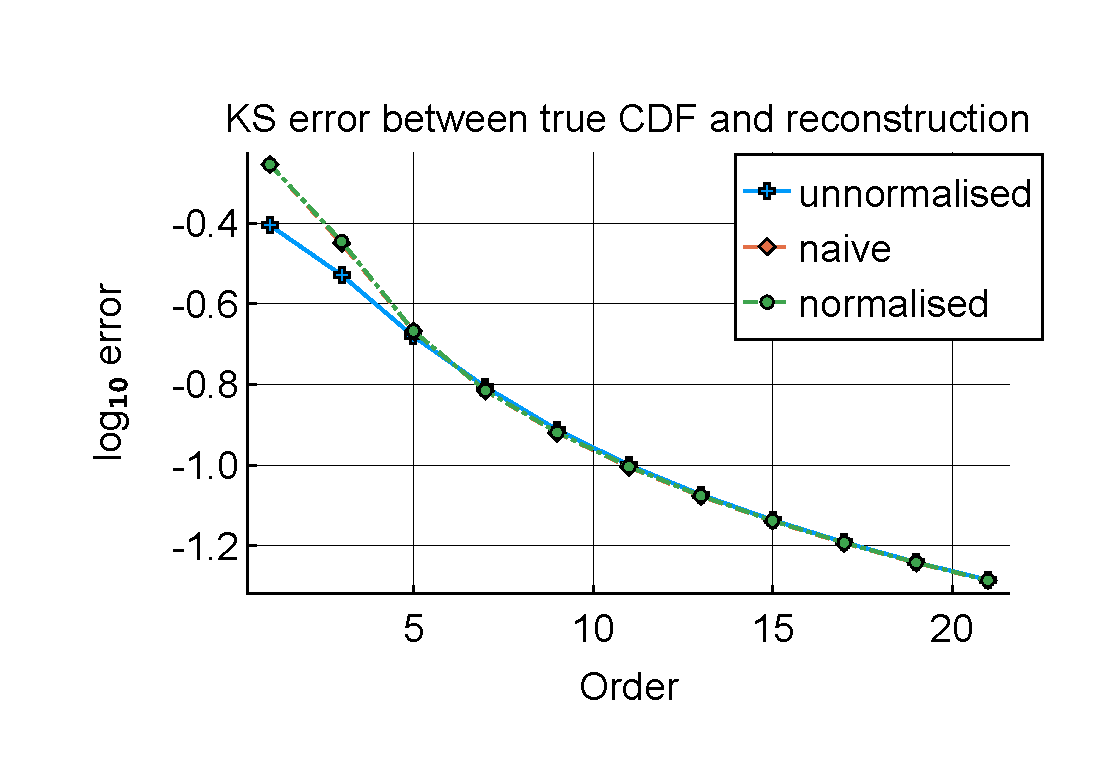
\includegraphics[width=0.5\textwidth,trim={1.25cm 0.8cm 0.25cm 1.25cm},clip]{chapter6/figs/qbdrap_closing_vec/fun2/ks_error_formatted.pdf}%
	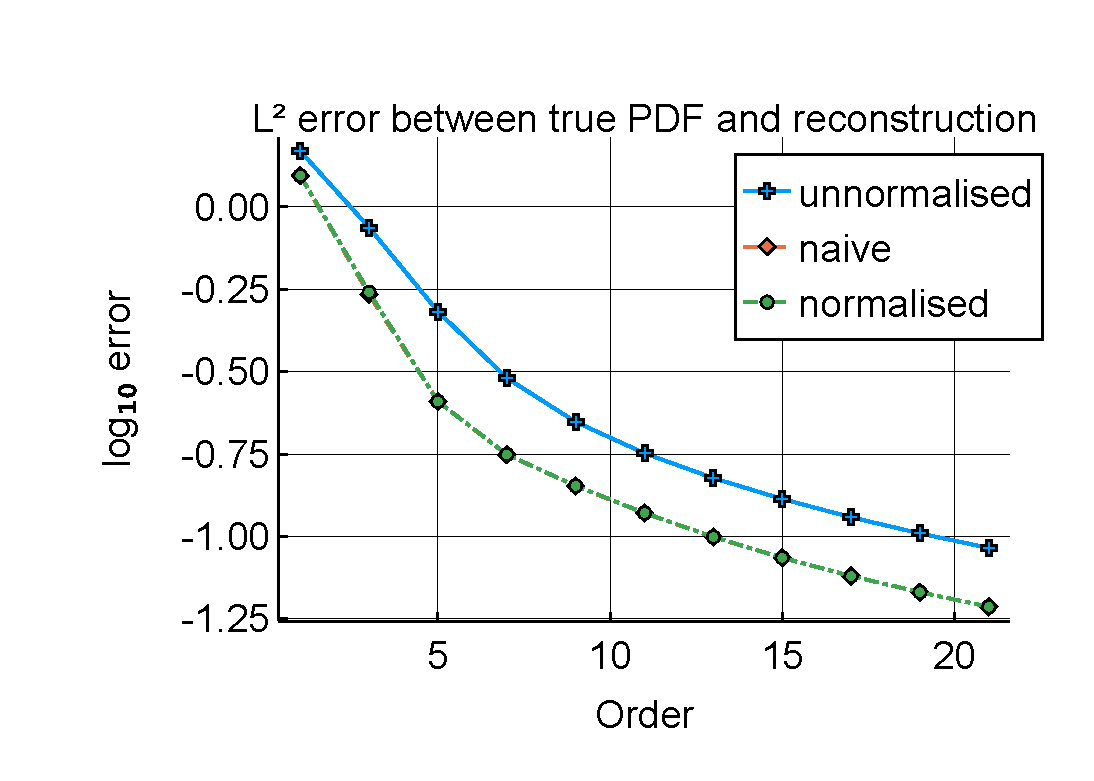
\includegraphics[width=0.5\textwidth,trim={1.25cm 0.8cm 0.25cm 1.25cm},clip]{chapter6/figs/qbdrap_closing_vec/fun2/l2_pdf_error_formatted.pdf}
	\caption{KS error between the true CDF, \(2x1(x<0.5)+1(x\geq 0.5)\), and the approximations (left) and \(L^2\) error between the true PDF, \(2\times 1(x<0.5)\), and the approximations (right) for the three closing vectors considered; unnormalised (blue solid line with crosses), naive normalised (orange dashed line with diamonds) and normalised (green dash-dotted line with circles). The naive normalised (orange) an normalised closing vectors are coincident.}
	\label{fig: fun 2 ks error qbdrap closing vecs}
\end{figure}
\exampleFloatBarrier
\end{example}

\begin{example}Now consider approximating the initial density \(f(x)=1\). Observing Figure~\ref{fig: fun 4 ks error qbdrap closing vecs} of the KS error and \(L^2\) error of the PDF we now see that the normalised reconstructions outperform the unnormalised reconstruction. This suggests that, in this case, the `folding' of closing operator about \(\Delta\) has greatly increased the ability of the reconstruction to approximate this initial distribution. 
\begin{figure}[h]
	\centering
	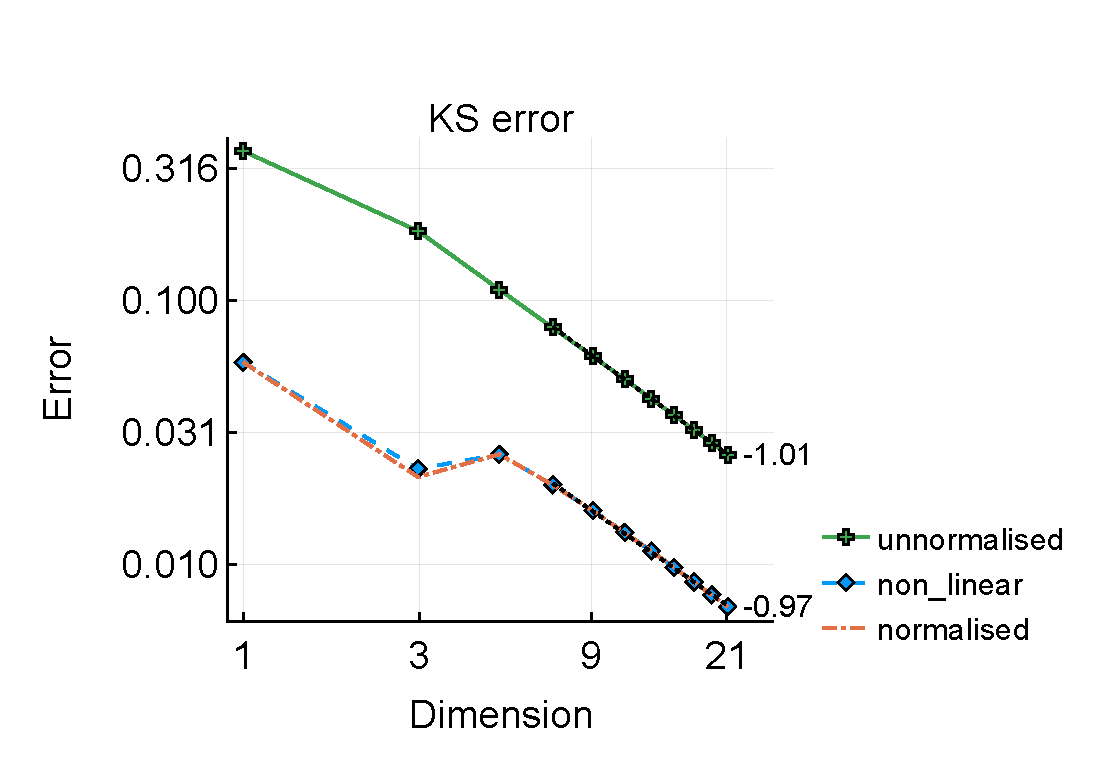
\includegraphics[width=0.5\textwidth,trim={1.25cm 0.8cm 0.25cm 1.25cm},clip]{chapter6/figs/qbdrap_closing_vec/fun4/ks_error_formatted.pdf}%
	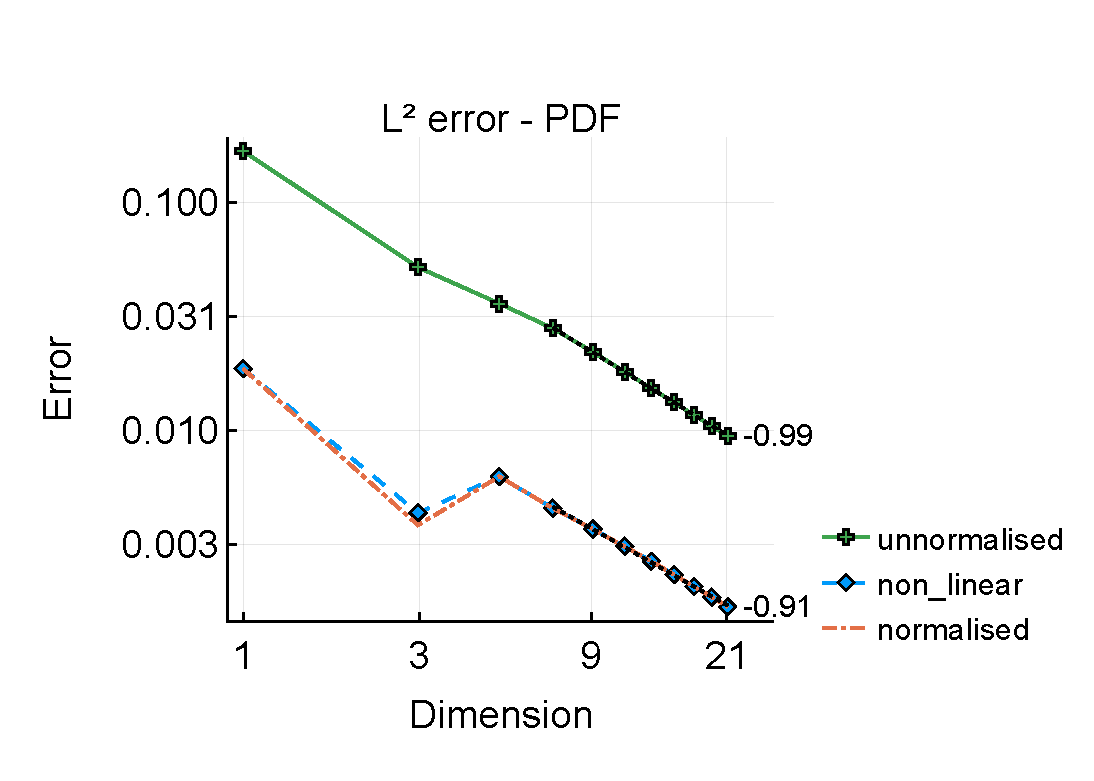
\includegraphics[width=0.5\textwidth,trim={1.25cm 0.8cm 0.25cm 1.25cm},clip]{chapter6/figs/qbdrap_closing_vec/fun4/l2_pdf_error_formatted.pdf}
	\caption{KS error between the true CDF, \(x\), and the approximation (left) and \(L^2\) error between the true PDF and the approximation (right) for the three closing vectors considered; unnormalised (blue solid line with crosses), naive normalised (orange dashed line with diamonds) and normalised (green dash-dotted line with circles). The naive normalised (orange) an normalised closing vectors are coincident.}
	\label{fig: fun 4 ks error qbdrap closing vecs}
\end{figure}

Some insight is gained by looking at Figure~\ref{fig: pdf reconstructed} where we plot the reconstructed PDFs for the unnormalised and normalised closing operators for dimension 1, 3, 5 and 7, as well as the true PDF. Observing Figure~\ref{fig: pdf reconstructed} notice that the unnormalised reconstruction fails to capture the density at the left of each of the plots. This feature is due to a significant amount of mass being lost due to the truncation. In comparison, the reconstruction with the normalised closing operator is much better in this region due to the `folding' around \(\Delta\) in the construction of the closing operator. The `folding' in the normalised closing operator manifest itself as more mass at the left of these plots compared to the unnormalised reconstructions. % Recall that, as discussed in Section~\ref{}, for the reconstruction we must to allocate the initial condition to a phase with positive rate, or negative rate, so that we can use the appropriate approximation and reconstruction method as discussed in Section~\ref{sec: closing}. Here we suppose that the phase is positive, so the `folding' around \(\Delta\) in the normalised closing operators appears appears at the left of the plots. In general, reconstructions via the unnormalised closing operator typically underestimate the value of the function in this region. 

Figure~\ref{fig: pdf reconstructed} also show that both closing operators do not approximate the initial condition well at the right-hand side of the interval. Perhaps there is a different reconstruction method or yet another closing operator which could alleviate this issue. 
\begin{figure}[h]
	\centering
	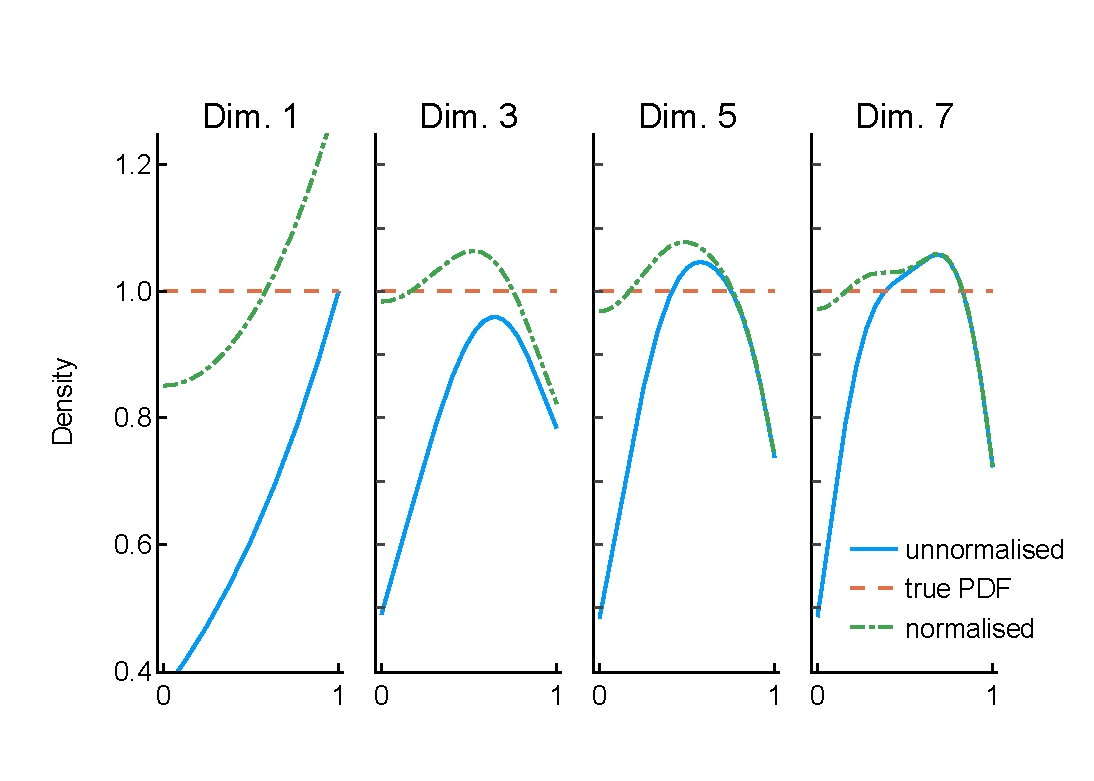
\includegraphics[width=\textwidth,trim={0cm 1.25cm 0cm 1.25cm},clip]{chapter6/figs/qbdrap_closing_vec/fun4/pdfs_formatted.pdf}
	\caption{Reconstructed PDFs using the unnormalised closing operator (blue solid line), normalised closing operator (green dash-dotted line), for various dimensions, and the true PDF which is \(f(x)=1\) (orange dashed line).}
	\label{fig: pdf reconstructed}
\end{figure} 
\exampleFloatBarrier
\end{example}

\begin{example}Next we consider approximating the initial distribution with density \(-6x^2+6x\). Observing the left-hand panel of Figure~\ref{fig: fun 6 ks error qbdrap closing vecs}, which plots the KS error against the dimension of the reconstruction for the three closing operators, we once again see that the reconstruction using the unnormalised closing operator performs the worst, while the performance of the two normalised reconstructions is indistinguishable. However, if we instead look at the right-hand panel of Figure~\ref{fig: fun 6 ks error qbdrap closing vecs}, which plots the \(L^2\) error between the reconstructed PDF and the true PDF, then the unnormalised closing operator performs better than the two normalised ones for dimension 5 and above. 
\begin{figure}[h]
	\centering
	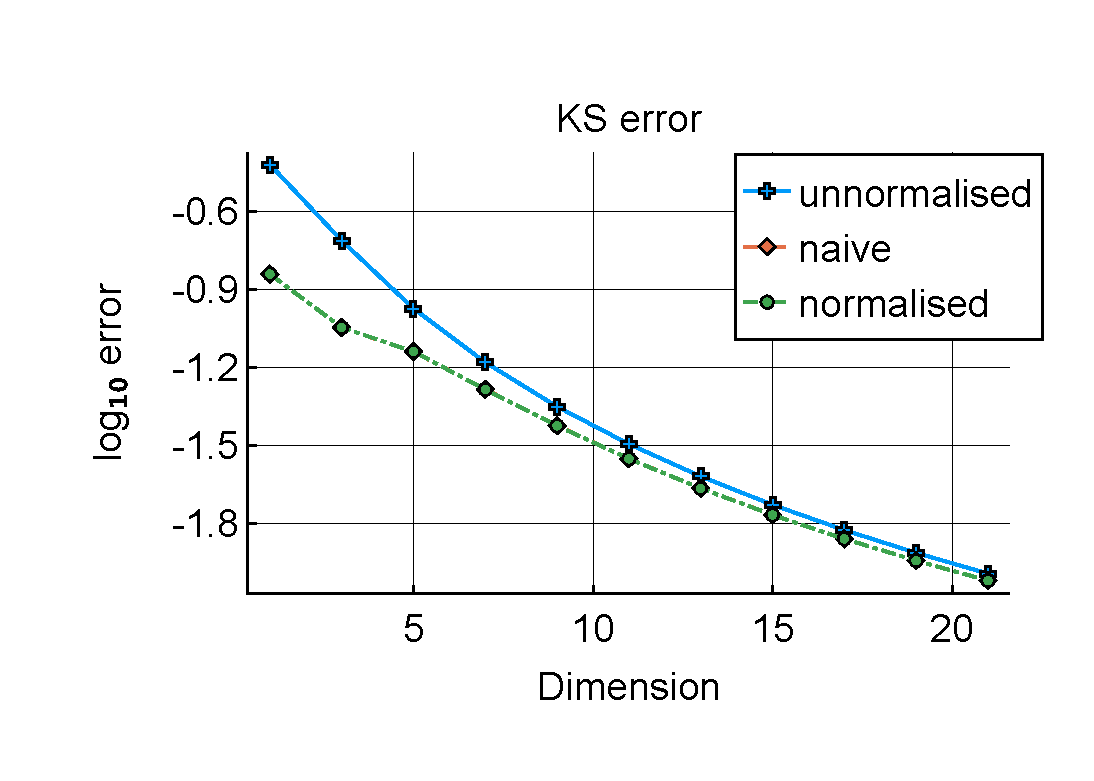
\includegraphics[width=0.5\textwidth,trim={1.25cm 0.8cm 0.25cm 1.25cm},clip]{chapter6/figs/qbdrap_closing_vec/fun6/ks_error_formatted.pdf}%
	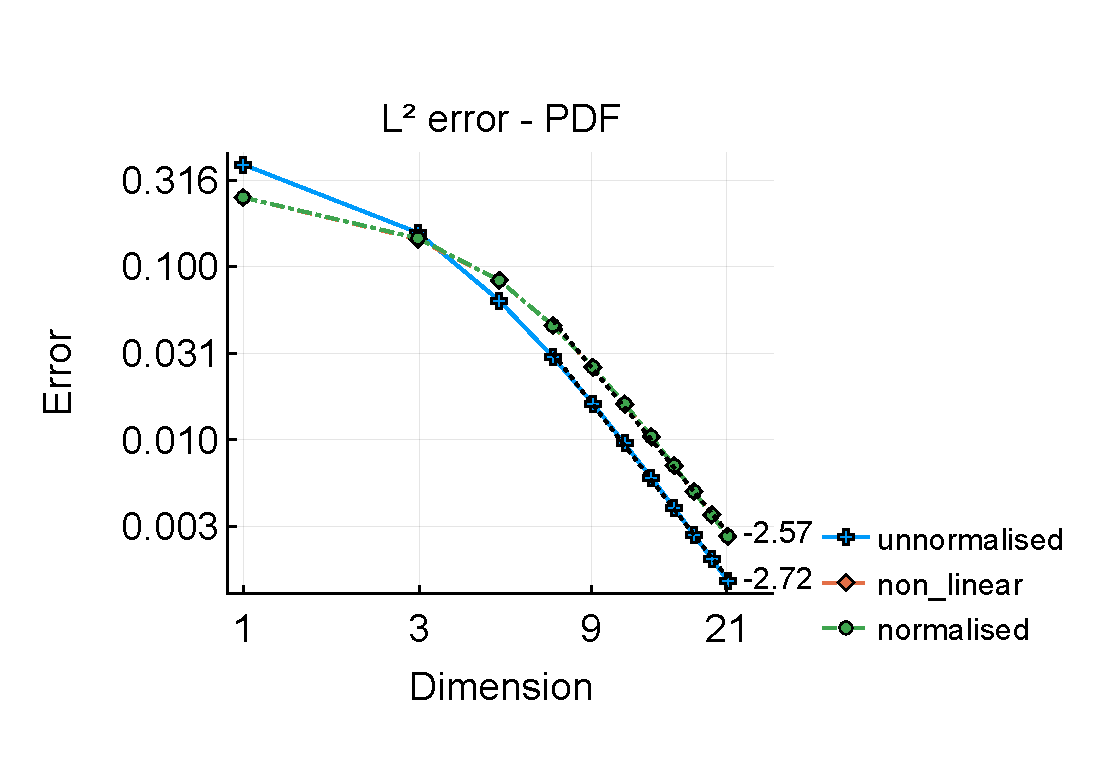
\includegraphics[width=0.5\textwidth,trim={1.25cm 0.8cm 0.25cm 1.25cm},clip]{chapter6/figs/qbdrap_closing_vec/fun6/l2_pdf_error_formatted.pdf}
	\caption{KS error between the true CDF, \(-2x^3+3x^2\), and the approximation (left) and \(L^2\) error between the true PDF \(-6x^2+6x\) and the approximation (right), for the three closing vectors considered; unnormalised (blue solid line with crosses), naive normalised (orange dashed line with diamonds) and normalised (green dash-dotted line with circles). The naive normalised (orange) an normalised closing vectors are coincident.}
	\label{fig: fun 6 ks error qbdrap closing vecs}
\end{figure}

The fact that the unnormalised closing operator outperforms the two normalised ones can be explained by the `folding' of the normalised operators around \(\Delta\). In Figure~\ref{fig: pdf reconstructed quadratic} we plot the unnormalised and normalised reconstructions along with the true PDF, \(-6x^2+6x\). In Figure~\ref{fig: pdf reconstructed quadratic} at the left of the plots, we observe that the normalised reconstructions over-estimate the density function, whereas the unnormalised reconstruction looks to be doing better. The `folding' in the normalised closing operator manifest itself as more mass at the left of these plots compared to the unnormalised reconstructions. 
\begin{figure}[h]
	\centering
	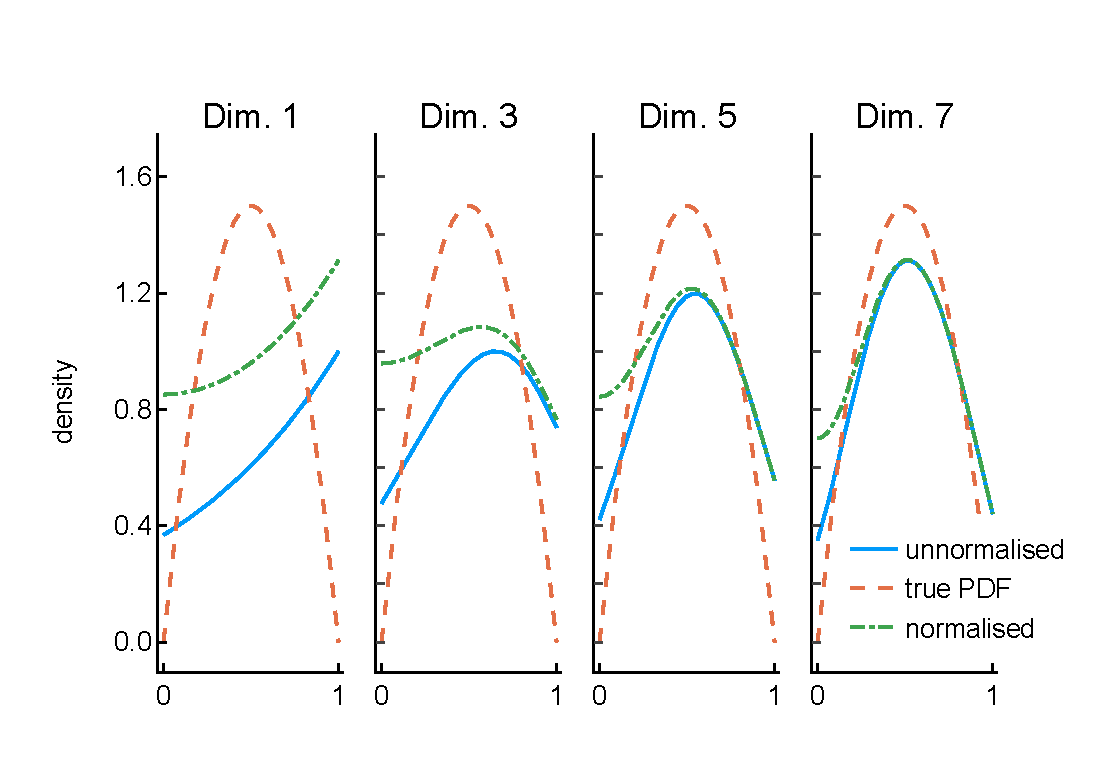
\includegraphics[width=\textwidth,trim={0cm 1.25cm 0cm 1.25cm},clip]{chapter6/figs/qbdrap_closing_vec/fun6/pdfs_formatted.pdf}
	\caption{Reconstructed PDFs using the unnormalised closing operator (blue solid line), normalised closing operator (green dash-dotted line), for various orders, and the true PDF which is \(f(x)=-6x^2+6x\) (orange dashed line).} 
	\label{fig: pdf reconstructed quadratic}
\end{figure} 
\exampleFloatBarrier
\end{example}

\begin{example}Lastly, we consider approximating the initial distribution with PDF \(3e^{-3x}/(1-e^{-3})\). This density function is at a maximum at the left of the region. Considering what we have learnt so far about the unnormalised operator underestimating in this region, we expect that the unnormalised closing operator will perform relatively poorly in this case. Indeed, observing Figures~\ref{fig: fun 7 ks error qbdrap closing vecs} we see that this is the case; the normalised reconstructions perform relatively well compared to the unnormalised reconstruction, as measured by both error metrics (KS statistic and \(L^2\) norm on the PDF). If we observed plots of the PDFs (omitted), we would once again see that this is due to the loss of mass at the left-hand side of the region due to the truncation. 
\begin{figure}[h]
	\centering
	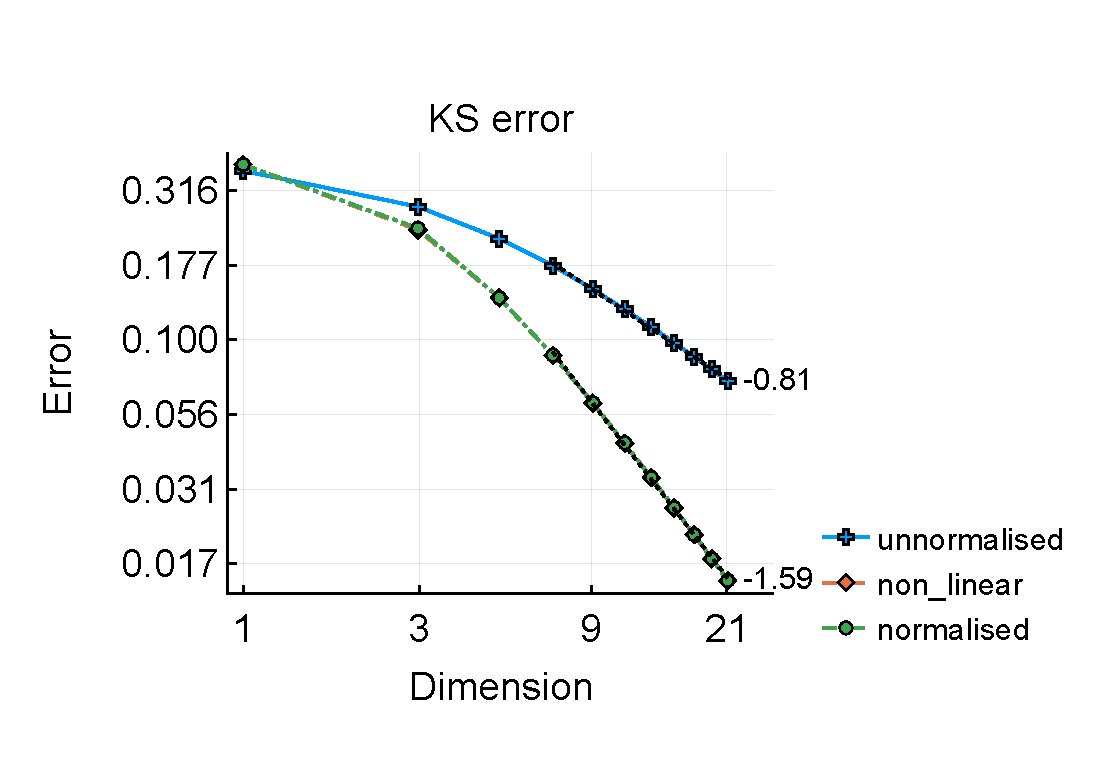
\includegraphics[width=0.5\textwidth,trim={1.25cm 0.8cm 0.25cm 1.25cm},clip]{chapter6/figs/qbdrap_closing_vec/fun7/ks_error_formatted.pdf}%
	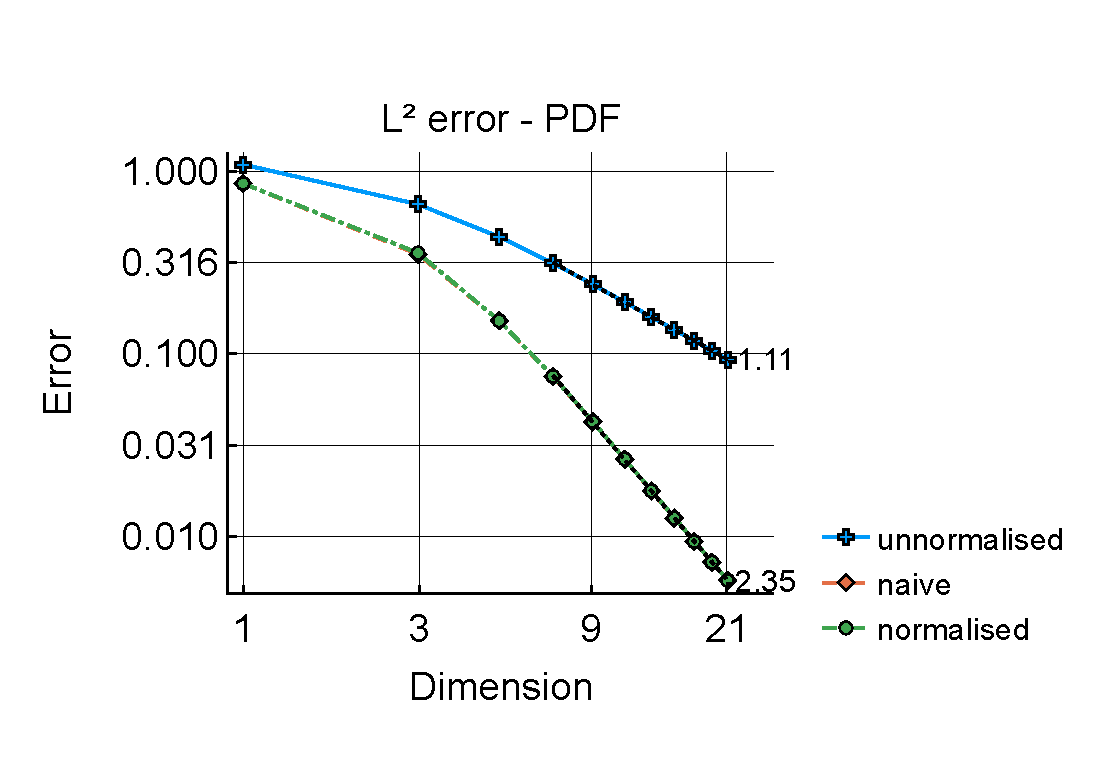
\includegraphics[width=0.5\textwidth,trim={1.25cm 0.8cm 0.25cm 1.25cm},clip]{chapter6/figs/qbdrap_closing_vec/fun7/l2_pdf_error_formatted.pdf}
	\caption{KS error between the true CDF, \((1-e^{-3x})/(1-e^{-3})\), and the approximation (left) and \(L^2\) error between the true PDF and the approximation for the three closing vectors considered; unnormalised (blue solid line with crosses), naive normalised (orange dashed line with diamonds) and normalised (green dash-dotted line with circles). The naive normalised (orange) and normalised closing vectors are coincident.}
	\label{fig: fun 7 ks error qbdrap closing vecs}
\end{figure}
\exampleFloatBarrier
\end{example}

Given the evidence above we choose to use the normalised closing operator to reconstruct solutions. Further, unlike the naive normalised operator, the normalised operator is theoretically justified in that we proved the closing operator leads to a convergent scheme and is linear. 

\FloatBarrier
\subsection{Comparison of methods}\label{sec: comp}
Here we compare the ability of the QBD-RAP, uniformisation, and DG methods to reconstruct initial conditions. 

\begin{example}First we consider the initial condition with CDF \(1(x\geq 0.5)\), that is, a point mass at 0.5. This distribution does not have a PDF, so we compare the CDFs only. In Figure~\ref{fig: fun 1 comp} we plot the KS metric (left) and \(L^1\) metric (right) between the true CDF and the reconstructed approximations. Observing the KS metric, it appears that none of the methods converge and the KS error sits around 0.5. This reflects the fact that convergence in distribution implies point-wise convergence of the CDFs except, perhaps, at points of discontinuity. None of the methods appear to converge at the discontinuity at \(x=0.5\). Observing the \(L^1\) error between the true CDF and reconstructed approximation (which is the area between the two CDFs) we now see that the methods appear to show the convergent behaviour we expect. Here, the uniformisation method appears to perform the best, while the QBD-RAP method performs the worst. The rate of convergence of the QBD-RAP method appears to be similar to the rate of convergence of the DG scheme. 

Perhaps it is no surprise that the uniformisation method performs best. In the uniformisation method as we increase the order we partition the cell \([0,1]\) into smaller sub-cells, and use constant functions on each sub-cell to approximate the initial distribution. As such, the uniformisation method can produce a piecewise continuous, linear approximation to the CDF. In contrast, both the DG and QBD-RAP methods result in a smooth approximation to the CDF. Given the initial distribution is far from smooth (it's a point mass), then we might expect that the uniformisation method will perform relatively well.
\begin{figure}[h]
	\centering
	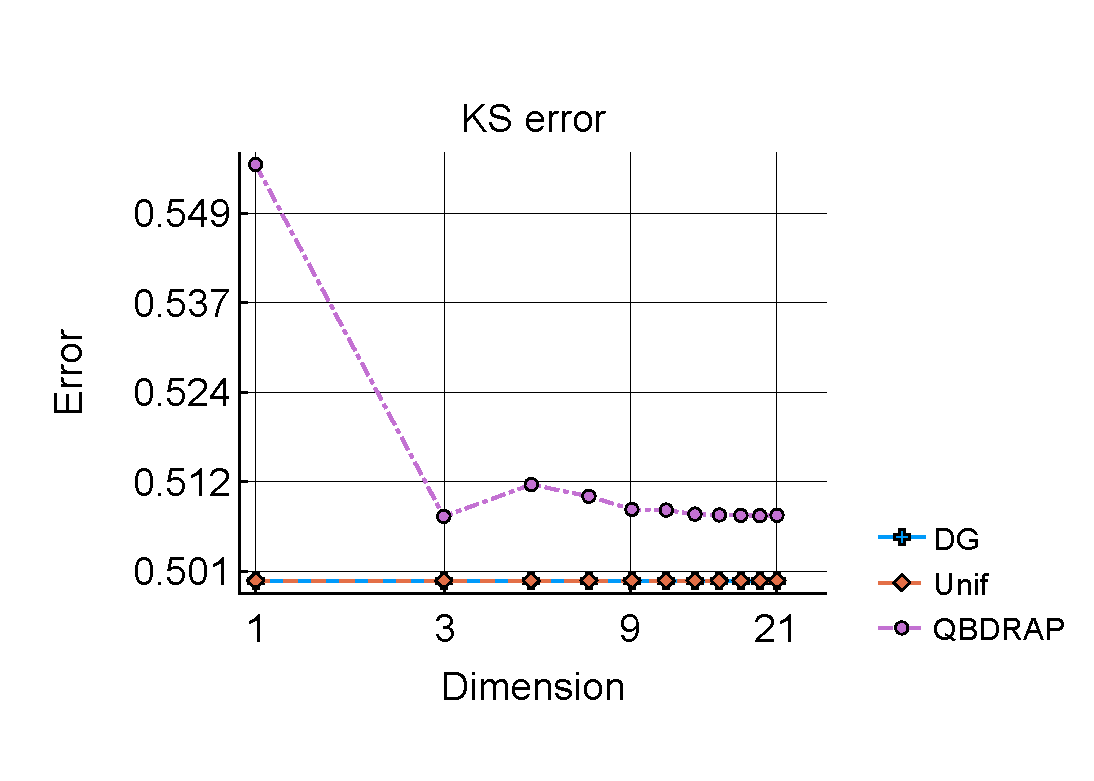
\includegraphics[width=0.5\textwidth,trim={1.25cm 0.8cm 0.25cm 1.25cm},clip]{chapter6/figs/comp/fun1/meshs_ks_error_formatted.pdf}%
	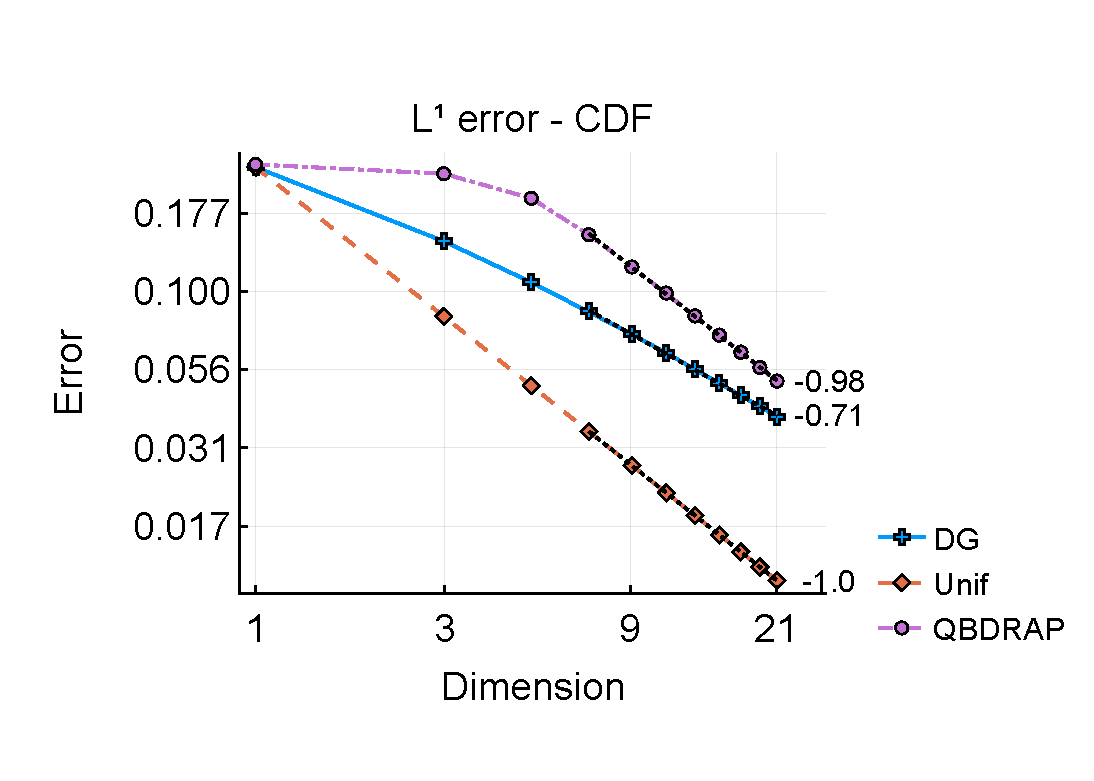
\includegraphics[width=0.5\textwidth,trim={1.25cm 0.8cm 0.25cm 1.25cm},clip]{chapter6/figs/comp/fun1/meshs_l1_cdf_error_formatted.pdf}
	\caption{KS error between the true CDF, \(1(x\geq 0.5)\), and the approximations (left) and \(L^1\) error between the true CDF and the approximations for the DG method (blue solid line with crosses), uniformisation method (orange dashed line with diamonds) and QBD-RAP method (purple dashed line with circles).}
	\label{fig: fun 1 comp} 
\end{figure}

In Figure~\ref{fig: pdf comp fun 1} we plot approximated CDFs from the DG, uniformisation and QBD-RAP methods alongside the true CDF. The DG method displays undesirable features for an approximation to a CDF -- it is not monotonically increasing, at some points it is negative and at some points it is above 1. On the other hand, although the QBD-RAP method converges slowest, it displays good properties in that it results in a monotonically increasing CDF, starting at 0 and ending at 1. The uniformisation scheme approximates the CDF exceptionally well.
\begin{figure}[h]
	\centering
	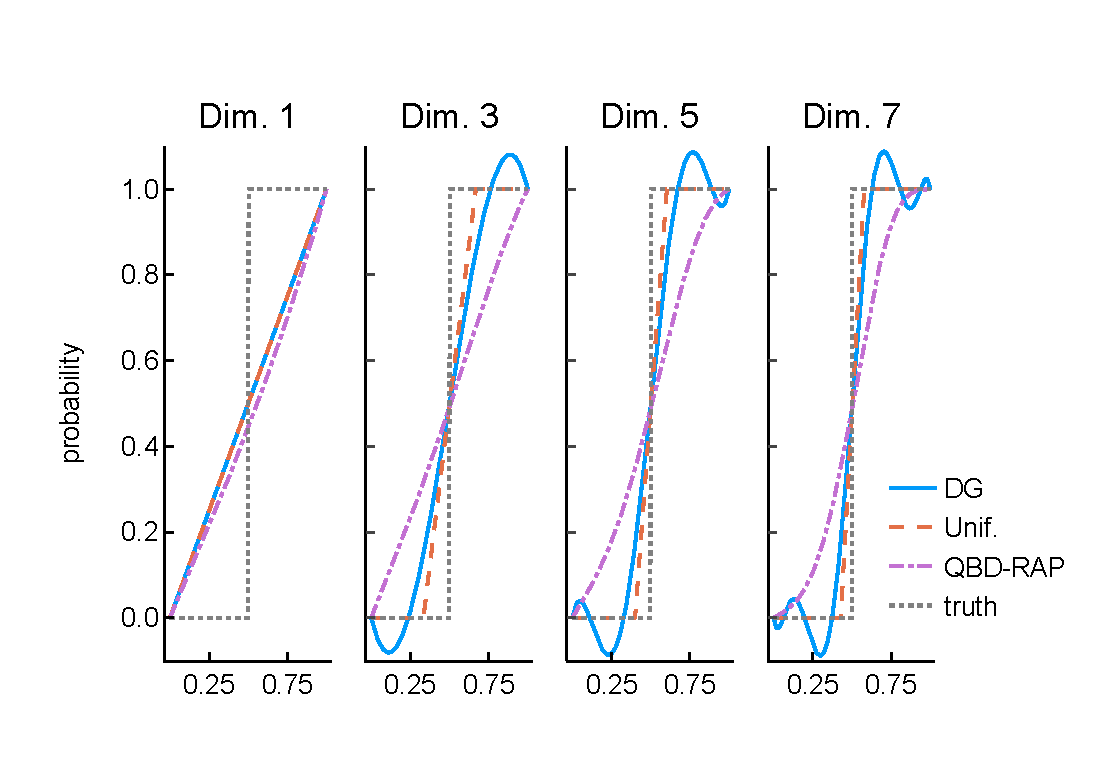
\includegraphics[width=\textwidth,trim={0cm 1.25cm 0cm 1.25cm},clip]{chapter6/figs/comp/fun1/cdfs_formatted.pdf}
	\caption{Reconstructed CDFs using the DG (blue solid line), uniformisation (orange dashed line) and QBD-RAP (purple dashed line) methods. The true distribution function is \(1(x\geq 0.5)\) (grey dotted line).}
	\label{fig: pdf comp fun 1}
\end{figure} 
\exampleFloatBarrier
\end{example}

\begin{example}Now consider approximating the initial distribution with PDF \(1(x\leq 0.5)\). Figure~\ref{fig: fun 2 comp} plots the KS error (left) and \(L^2\) error between the true and approximate PDFs (right). Figure~\ref{fig: fun 2 comp} suggests that all methods converge at a similar rate for this problem. Here, the QBD-RAP method performs worst, the uniformisation method second, and the DG method the best. However, once again the DG method exhibits undesirable properties (plots not shown) -- the approximation to the CDF is at some points above 1 and is not monotonic (although these violations do not appear to be as severe in this case as they were for the example above). 
\begin{figure}[h]
	\centering
	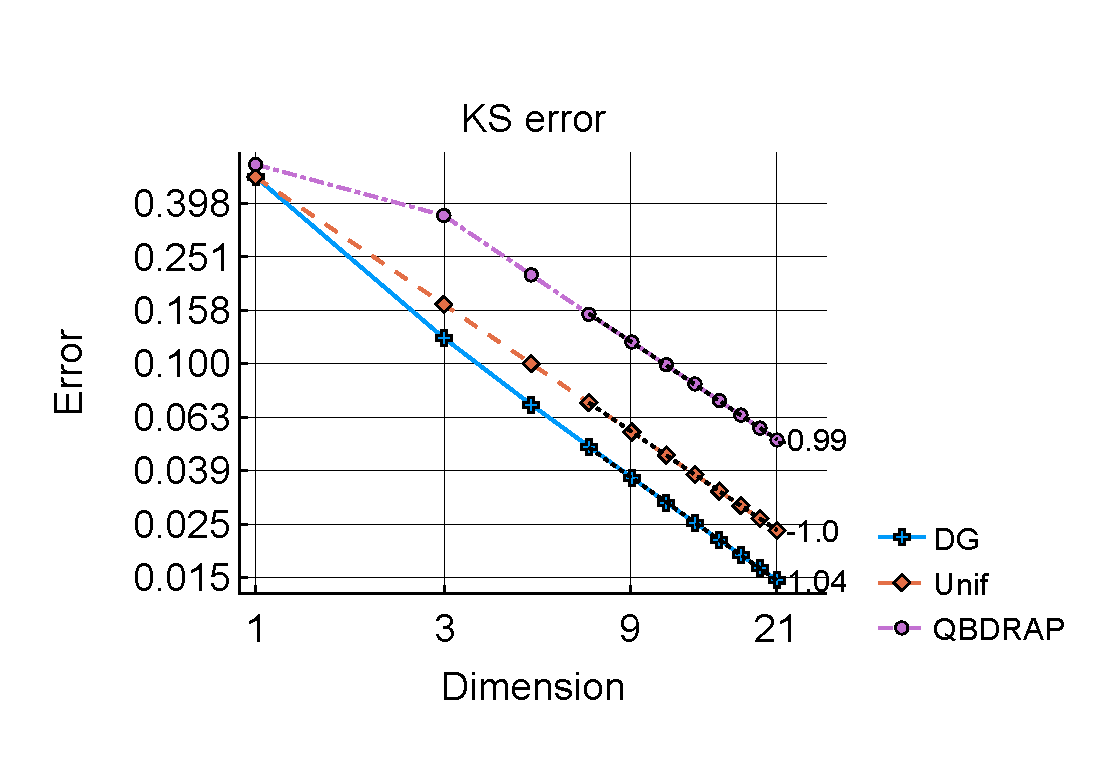
\includegraphics[width=0.5\textwidth,trim={1.25cm 0.8cm 0.25cm 1.25cm},clip]{chapter6/figs/comp/fun2/meshs_ks_error_formatted.pdf}%
	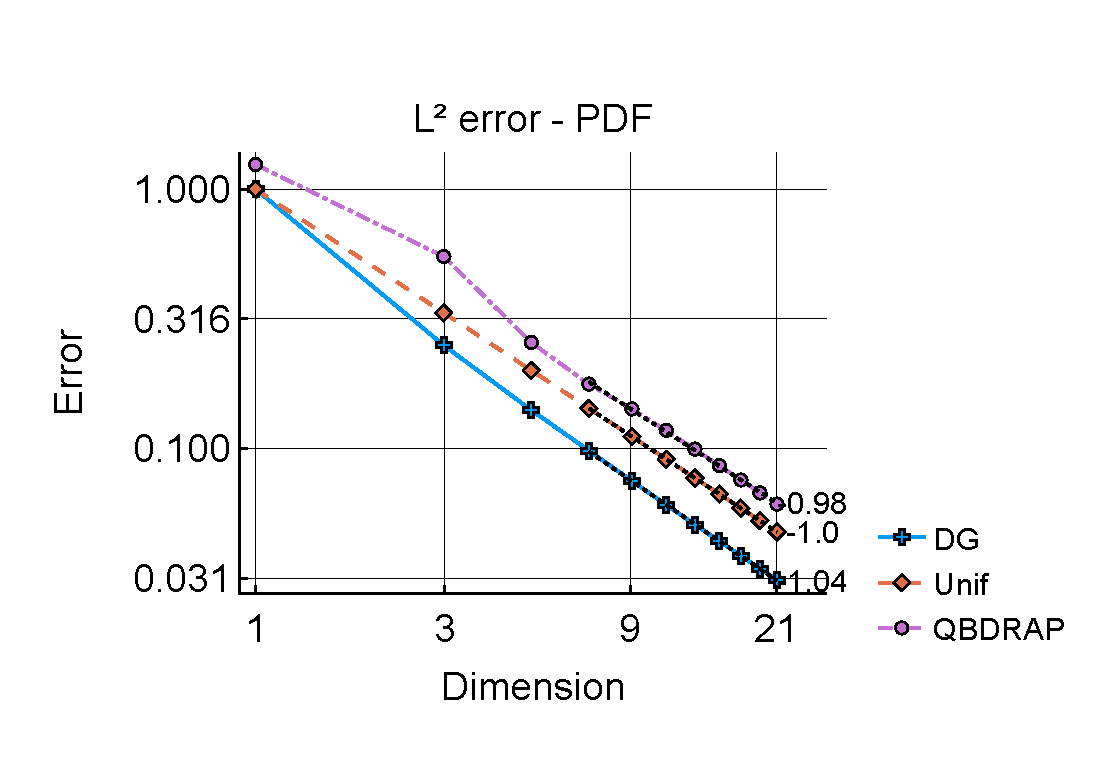
\includegraphics[width=0.5\textwidth,trim={1.25cm 0.8cm 0.25cm 1.25cm},clip]{chapter6/figs/comp/fun2/meshs_l2_pdf_error_formatted.pdf}
	\caption{KS error between the true CDF and the approximations (left) and \(L^2\) error between the true PDF, \(1(x\geq 0.5)\), and the approximations for the DG method (blue solid line with crosses), uniformisation method (orange dashed line with diamonds) and QBD-RAP method (purple dashed line with circles).}
	\label{fig: fun 2 comp} 
\end{figure}
\exampleFloatBarrier
\end{example}

\begin{example}So far we have considered two problems which exhibit discontinuities. At the other extreme we now consider an initial distribution with density \(-6x^2+6x\). In Figure~\ref{fig: fun 6 comp} we plot the KS error and the \(L^2\) error between the true and approximated PDFs. Since the DG method projects the initial condition onto a polynomial basis, then, for an order 3 approximation and above, the DG method can approximate the initial condition exactly. This is reflected in Figure~\ref{fig: fun 6 comp}, where the blue curve drops sharply from dimension 1 to 3, then plateaus. Due to numerical integration errors, for example in the evaluation of the integral in the \(L^2\) norm, and due to machine arithmetic, the errors for the DG scheme are not 0. Regarding the other two methods, they too appear to be convergent at approximately the same rate, with the uniformisation method performing better for the KS error, but very similarly in terms of the \(L^2\) error. 
\begin{figure}[h]
	\centering
	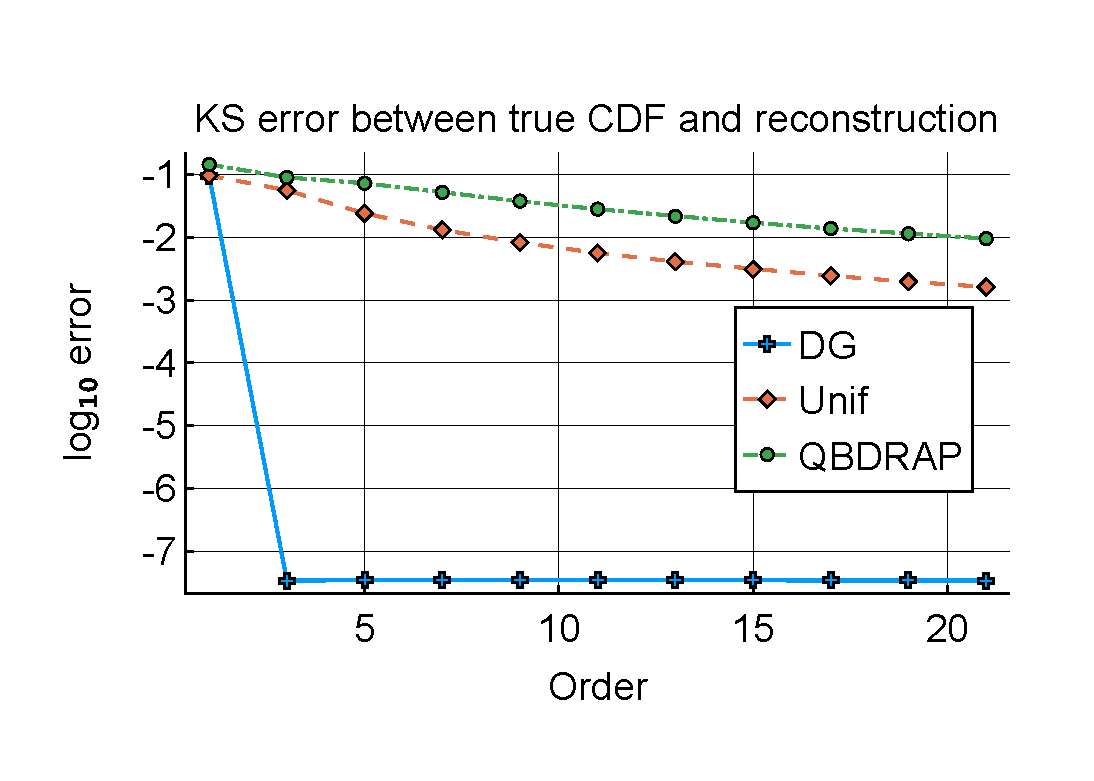
\includegraphics[width=0.5\textwidth,trim={1.25cm 0.8cm 0.25cm 1.25cm},clip]{chapter6/figs/comp/fun6/meshs_ks_error_formatted.pdf}%
	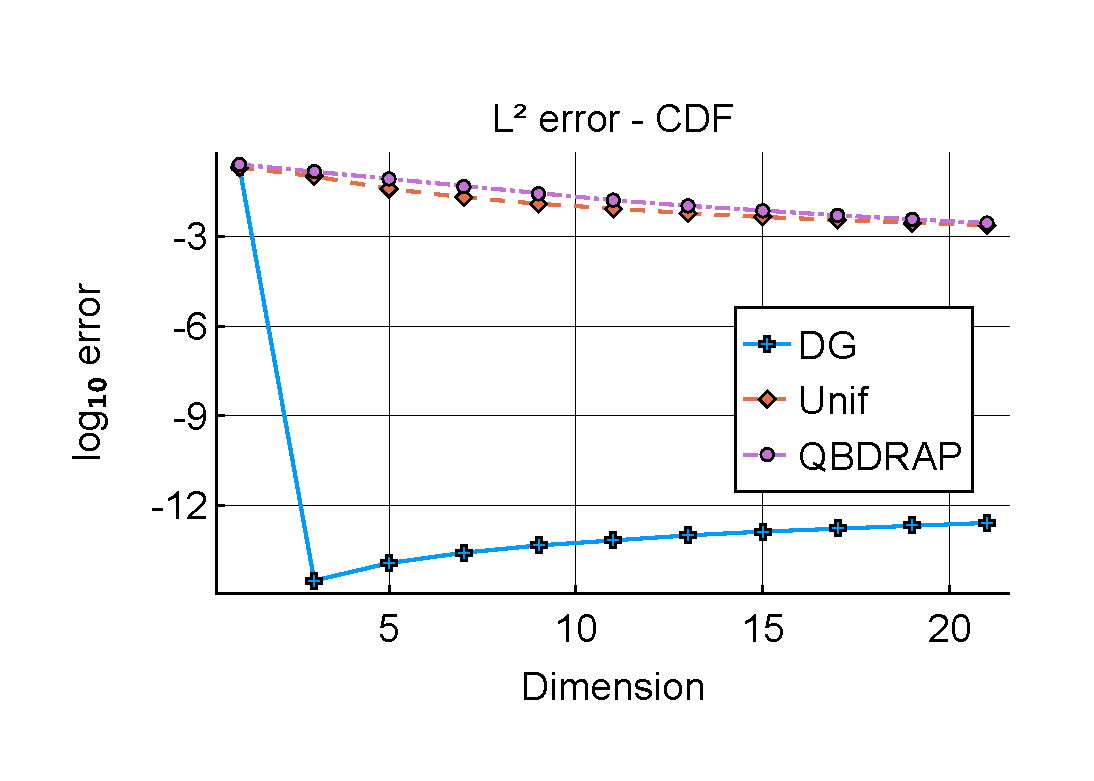
\includegraphics[width=0.5\textwidth,trim={1.25cm 0.8cm 0.25cm 1.25cm},clip]{chapter6/figs/comp/fun6/meshs_l2_pdf_error_formatted.pdf}
	\caption{KS error between the true CDF and the approximations (left) and \(L^2\) error between the true PDF, \(-6z^2+6x\), and the approximations for the DG method (blue solid line with crosses), uniformisation method (orange dashed line with diamonds) and QBD-RAP method (purple dashed line with circles).}
	\label{fig: fun 6 comp} 
\end{figure}
\exampleFloatBarrier
\end{example}

\begin{example}Consider now the initial distribution with PDF \(cos(4\pi(x+0.5))+1\). Figure~\ref{fig: fun 9 comp} shows the errors. Both the KS error (left) and \(L^2\) norm between the true and approximated PDFs (right) tell a similar story; for sufficiently high order, the DG method approximates the initial condition very well. The uniformisation method performs second best, while the QBD-RAP method is slowest to converge. 
\begin{figure}[h]
	\centering
	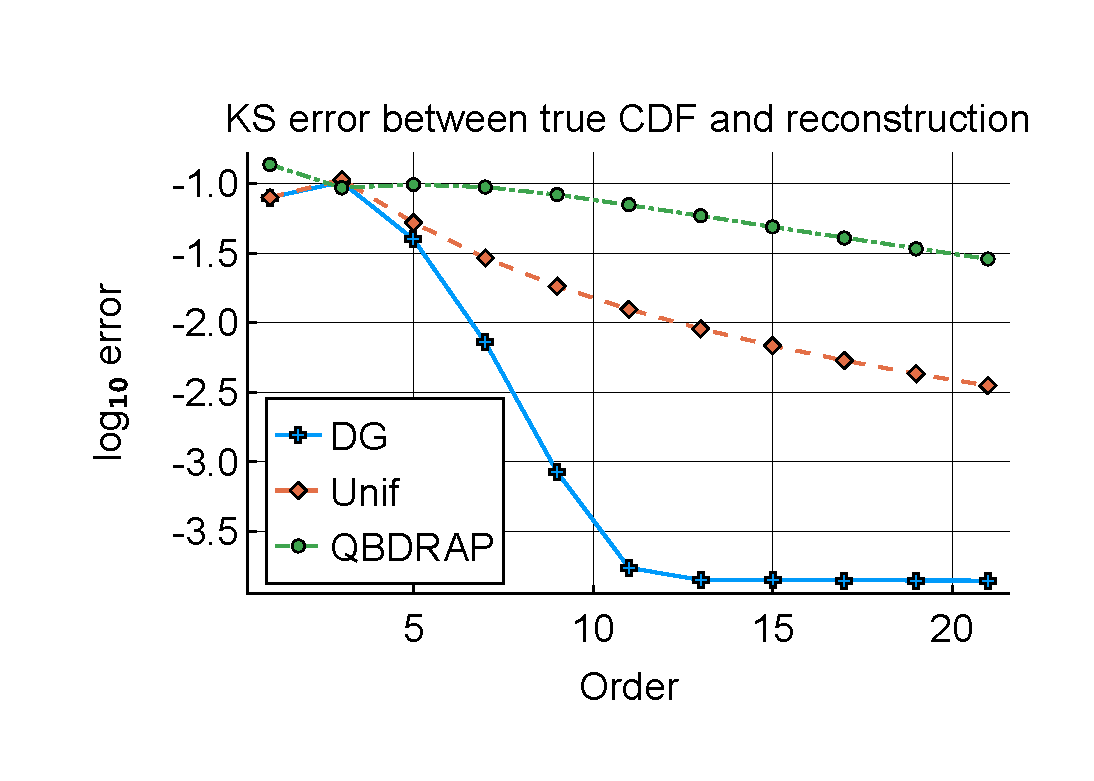
\includegraphics[width=0.5\textwidth,trim={1.25cm 0.8cm 0.25cm 1.25cm},clip]{chapter6/figs/comp/fun9/meshs_ks_error_formatted.pdf}%
	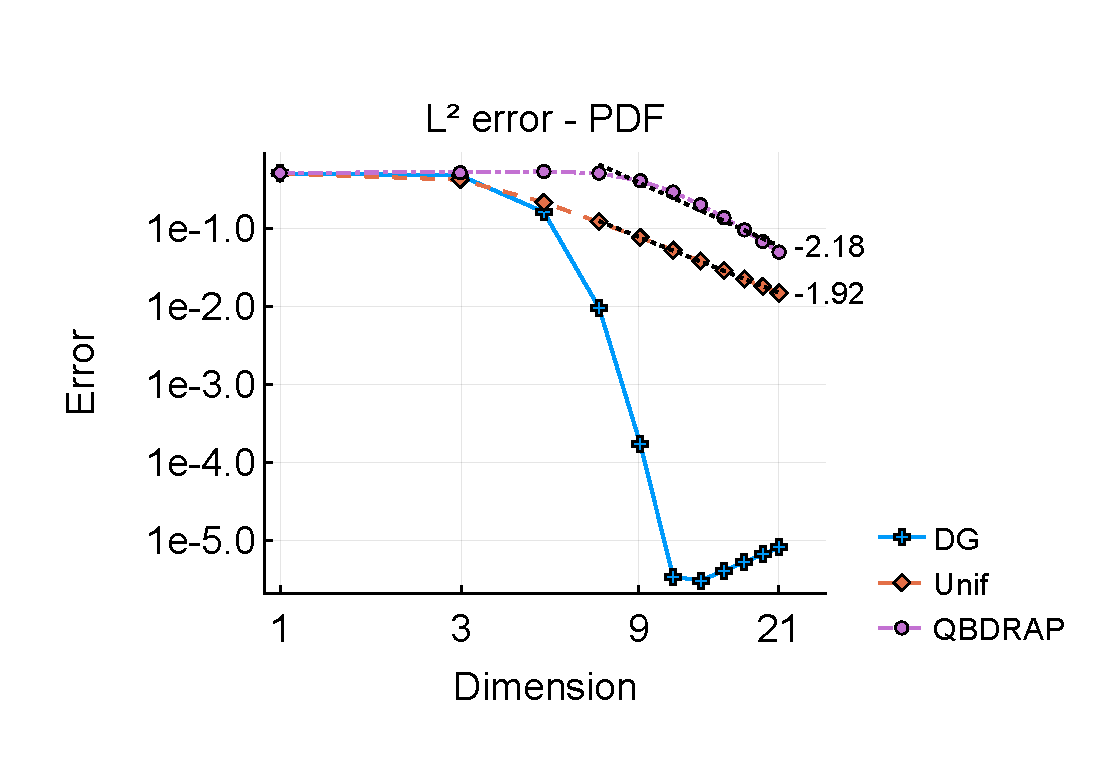
\includegraphics[width=0.5\textwidth,trim={1.25cm 0.8cm 0.25cm 1.25cm},clip]{chapter6/figs/comp/fun9/meshs_l2_pdf_error_formatted.pdf}
	\caption{KS error between the true CDF and the approximations (left) and \(L^2\) error between the true PDF, \(cos(4\pi(x+0.5))+1\), and the approximations for the DG method (blue solid line with crosses), uniformisation method (orange dashed line with diamonds) and QBD-RAP method (purple dashed line with circles).}
	\label{fig: fun 9 comp} 
\end{figure}
\exampleFloatBarrier
\end{example}

In conclusion, we have observed that the DG method performs well with respect to the error metrics considered, but can display oscillations and result in CDFs which are not non-decreasing. On the other hand, the uniformisation and QBD-RAP schemes result in non-decreasing approximations to the CDFs, but can converge slower with respect to the error metrics considered, with the QBD-RAP scheme often converging the slowest.
\FloatBarrier

\section{Travelling wave}\label{sec: wave num}
Here we investigate the performance the different schemes for approximating transient distributions of one-dimensional travelling wave problems with various initial conditions. Consider a (trivial) fluid queue with one phase, generator \(\bs T=[0]\) and rate \(c=1\). The PDE (if/when it exists) which describes this system is 
\[\cfrac{\partial}{\partial t} f(x,t) = -\cfrac{\partial}{\partial x} f(x,t),\]
where \(f(x,t)\) is the density at time \(t\). Given an initial condition, \(f(x,0)\), solutions to this problem are given by 
\[f(x,t) = f(x-t,0)\]
so the solution at time \(t\) is just a shift in the initial condition \(t\) units to the right. We suppose that the fluid queue is bounded, with a lower boundary \(x=0\) and upper boundary \(x=10\). This example is convenient as it has a known solution and no stochastic dynamics, hence we can instrument the ability of the schemes to approximate the flow of mass, without any stochastic dynamics. 

We use the QBD-RAP, uniformisation and DG schemes to discretise the solution in space. We discretise the interval \([0,10]\) into \(10\) cell, each of width 1. We use \(10,001\) points to approximate the integrals which appear in the construction of the initial conditions, to approximate the integrals appearing in the error metrics, and also as a set of discrete points on which evaluate the CDFs to approximate the KS metric. We use the SSPRK4 method to integrate over time with a \(t\)-step size of \(0.005\), and we evolve the system until time \(t=4\).\footnote{The \(t\)-step size must be chosen to ensure that numerical integration over time is stable up to dimension 21, adhering to a CFL-like condition \cite[Section~4.8]{nodalDGBook}.} For the DG method we also implement the Generalised MUSCL slope limiter to stabilise the integration \citep{c99}, \citep[Section~5.6.2]{nodalDGBook} (see also Section~\ref{sec: slope limiting}). 

To investigate the performance of the methods without the need to reconstruct the function within each cell we use the cell-wise error metric obtained by computing 
\begin{align}
	&\sum_{\ell=1}^{10} \left|\mathbb P(X(4)\in\calD_{\ell,1}, \varphi(4)=1\mid X(0)=0.5,\varphi(0)=1)-p(4,\ell,1)\right|\nonumber 
	\\&+\left|\mathbb P(X(4)\in\{10\}, \varphi(4)=1\mid X(0)=0.5,\varphi(0)=1)-p(4,11,1)\right| \label{eqn: cell errors}
\end{align}
where 
\begin{align}
	\mathbb P(X(4)\in\calD_{\ell,1}, \varphi(4)=1\mid X(0)=0.5,\varphi(0)=1) \label{eqn: cell probs}
\end{align}
for \(\ell=1,\dots,K\), and 
\begin{align}
	\mathbb P(X(4)\in\{10\}, \varphi(4)=1\mid X(0)=0.5,\varphi(0)=1) \label{eqn: cell probs boundary}
\end{align}
is the mass at the boundary and where \(p(4,\ell,1)\) is an approximation to \(\mathbb P(X(4)\in\calD_{\ell,1}, \varphi(4)=1\mid X(0)=0.5,\varphi(0)=1)\), and \(p(4,11,1)\) is an approximation to \(\mathbb P(X(4)\in\{10\}, \varphi(4)=1\mid X(0)=0.5,\varphi(0)=1)\).

\begin{example}\label{ex: wave 4}
First consider the initial condition with PDF \(1(x<1)\). The level of the fluid queue is uniformly distributed over the first cell. For the DG and uniformisation methods, the initial condition can be represented exactly, whereas, for the QBD-RAP method, it cannot. Thus, in this case, there is no discretisation error in constructing the initial condition for the DG and uniformisation methods. At time \(t=4\), the solution is \(f(x,4)=1(x\in[4,5))\). The projections related to the DG and uniformisation methods can represent this solution exactly too, hence we might expect these methods to work well here. 

We plot the cell-wise error metric in Figure~\ref{fig: fun 4 wave cp} and observe that the DG method appears to converge fastest, followed by the QBD-RAP method, then the uniformisation method, and the DG scheme with a slope limiter does not appear to converge. The DG scheme with a slope limiter has detected oscillations in the approximate solution and reduced the scheme to linear where oscillations are detected, thereby decreasing the accuracy of the scheme to linear where oscillations are present. 
\begin{figure}[h]
	\centering
	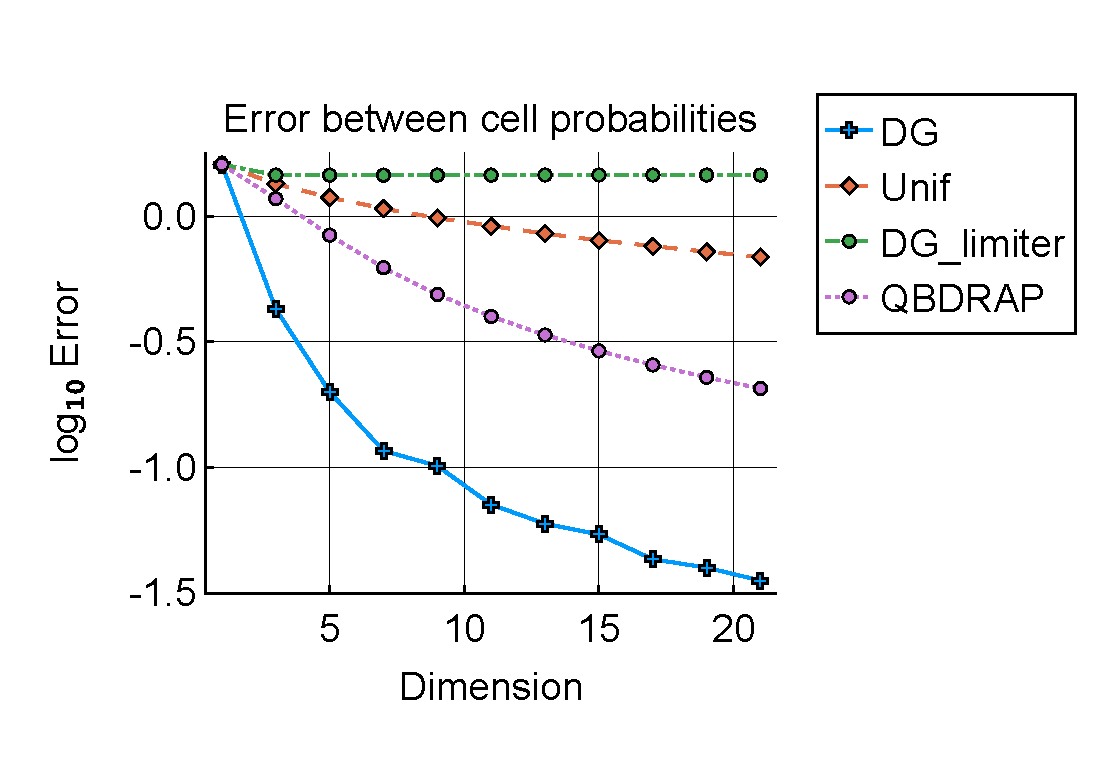
\includegraphics[width=0.5\textwidth,trim={0.75cm 0.8cm 0.25cm 1.25cm},clip]{chapter6/figs/wave/fun4/L1_cell_probs.pdf}
	\caption{Cell-wise error defined in (\ref{eqn: cell errors}) for the travelling wave in Example~\ref{ex: wave 4}. Plotted are the cell-wise errors for the DG method (blue solid line), DG method with Generalised MUSCL limiter (green dashed line), uniformisation method (orange dashed line) and QBD-RAP method (purple dotted line) versus the dimension of the approximation.}
	\label{fig: fun 4 wave cp} 
\end{figure}

Figure~\ref{fig: fun 4 wave} plots the KS error between the approximated and true CDFs and \(L^2\) error between the approximated and true PDFs. Comparing Figure~\ref{fig: fun 4 wave cp} with Figure~\ref{fig: fun 4 wave}, each method seems to show a similar rate of decay for error metrics with and without reconstruction. 

Returning to Figure~\ref{fig: fun 4 wave}, the DG method with the MUSCL limiter does not appear to converge with these error metrics for this problem (due to the limiter reducing the approximation to linear near the discontinuity), while the other two positivity preserving methods, the uniformisation and QBD-RAP schemes, both appear to be converging with the QBD-RAP method converging faster. With these error metrics, the DG method appears to be converging fastest. However, if we observe the approximations resulting from the DG method (Figure~\ref{fig: pdf wave fun 4} top-row), we find them to be unsatisfactory due to oscillations and negative values. 

Figure~\ref{fig: pdf wave fun 4} plots the density functions reconstructed using the DG, uniformisation, DG with MUSCL limiter and QBD-RAP methods for various dimension schemes. In the first row we observe that the DG method (sans limiter) produces an approximation to the PDF with negative values when the dimension is greater than 1. In the third row of Figure~\ref{fig: pdf wave fun 4} we observe that, with the limiter, the DG approximation does not change significantly after order 3. This is due the fact that the DG method is at best linear in the presence of oscillations. In the second row of Figure~\ref{fig: pdf wave fun 4} is the solution approximated using the uniformisation method, and in the last row is the solution approximated using the QBD-RAP method. 
\begin{figure}[h]
	\centering
	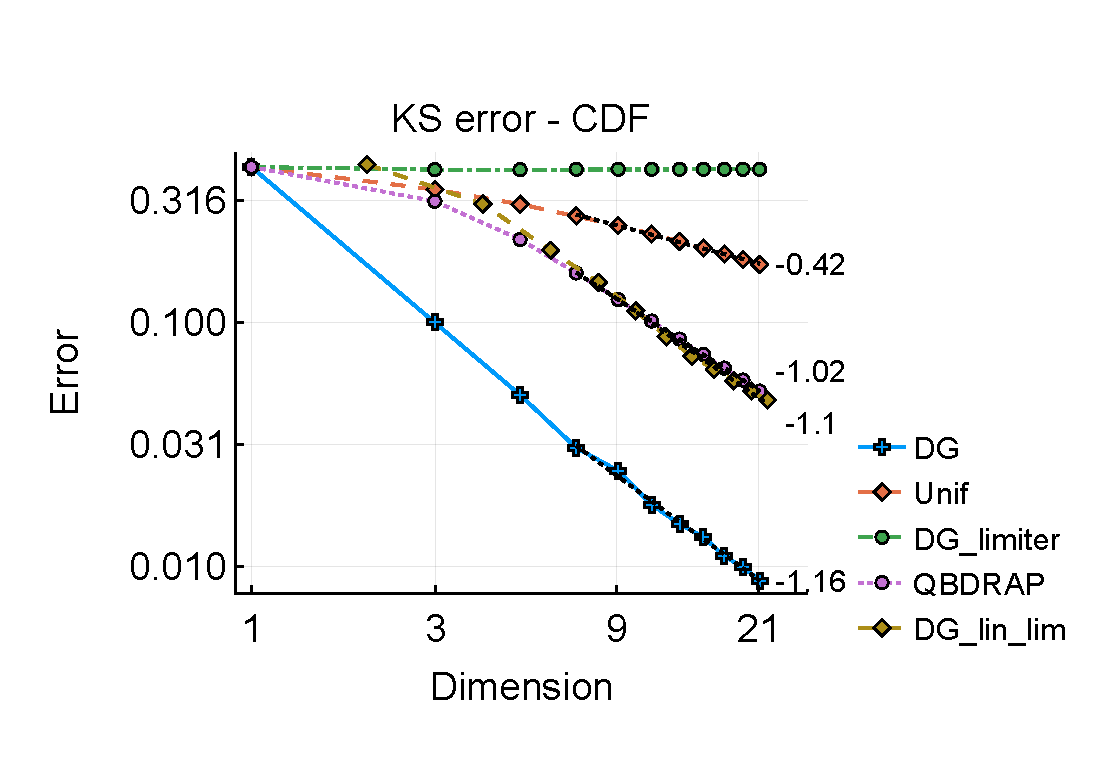
\includegraphics[width=0.5\textwidth,trim={0.75cm 0.8cm 0.25cm 1.25cm},clip]{chapter6/figs/wave/fun4/meshs_ks_error_formatted.pdf}%
	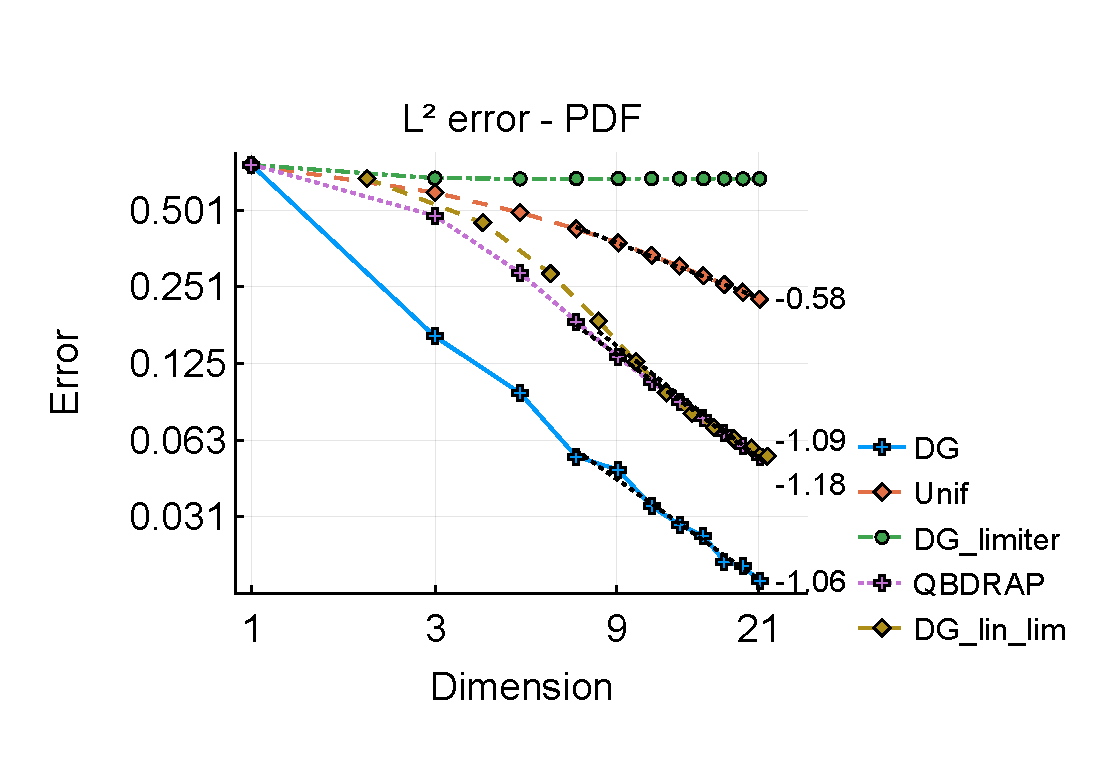
\includegraphics[width=0.5\textwidth,trim={0.75cm 0.8cm 0.25cm 1.25cm},clip]{chapter6/figs/wave/fun4/meshs_l2_pdf_error_formatted.pdf}
	\caption{KS error (left) and \(L^2\) error of the PDFs for the travelling eave problem in Example~\ref{ex: wave 4} using the approximations from the DG method (blue solid line with crosses), DG method with the MUSCL limiter (green dash-dotted line with crosses), uniformisation method (orange dashed line with diamonds) and QBD-RAP method (purple dotted line with circles).} 
	\label{fig: fun 4 wave} 
\end{figure}
\begin{figure}[h]
	\centering
	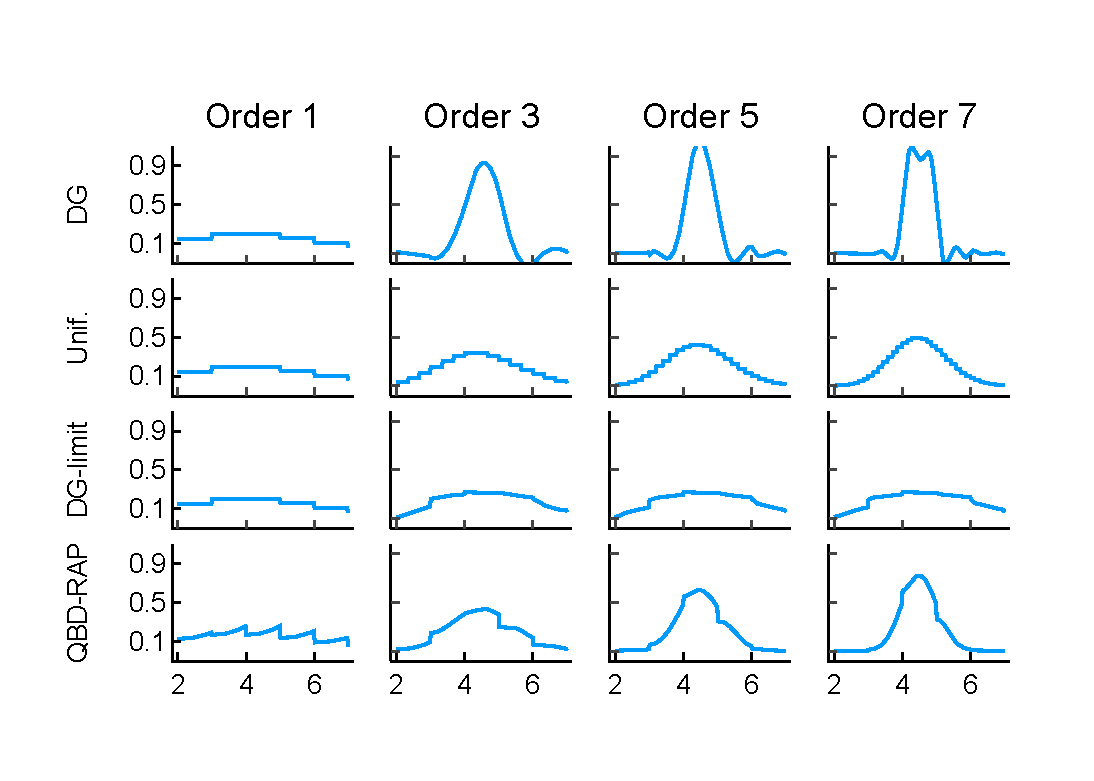
\includegraphics[width=\textwidth,trim={0cm 1.25cm 0cm 1.25cm},clip]{chapter6/figs/wave/fun4/pdfs_formatted.pdf}
	\caption{Reconstructed PDFs using the DG (top row), uniformisation (second row), DG with MUSCL limiter (third row) and QBD-RAP (bottom row) methods, for order 1, 3, 5, and 7 (columns) for the travelling eave problem in Example~\ref{ex: wave 4}. The true density function is \(1(4\leq x<5)\).}
	\label{fig: pdf wave fun 4}
\end{figure} 

This is a particularly interesting example. It shows that, for the DG method, even though there is no discretisation error for the initial condition, we use a strong stability preserving time-integration method, and the projection off which the DG method is based can represent the transient distribution at time \(t=4\) exactly, there is still the possibility of badly behaved solutions as in the top row of Figure~\ref{fig: pdf wave fun 4}. 
\exampleFloatBarrier
\end{example}

\begin{example}\label{ex: wave 2}
Another interesting example occurs with the initial condition with CDF \(1(x\geq 0.5)\), i.e.~a point mass at 0.5. The exact solution at time \(t=4\) is therefore a point mass at \(4.5\). No PDF exists for the true distribution, so instead we compare the CDFs. Moreover, when we analysed reconstruction of this initial condition we saw that using the KS metric may be uninformative. Instead, for this example, we measure errors by looking at the \(L^1\) error between the CDFs (the area between the CDFs) and the cell-wise error from (\ref{eqn: cell probs})-(\ref{eqn: cell errors}).

Figure~\ref{fig: fun 2 wave} (left) plots the \(L^1\) error between the true and approximated CDFs. The \(L^1\) metric tells a similar story to the previous analysis: the DG method with the limiter does not converge as order increases, the other two positivity preserving methods (the uniformisation and QBD-RAP methods) appear to converge, with the QBD-RAP method converging faster, while the DG method appears to converge the fastest. However, if we plot the approximations to the CDFs from the DG method (not shown) we would once again see an oscillating, non-monotonic function. Another interesting observation is to compare the performance of the uniformisation and QBD-RAP methods with respect to the \(L^1\) metric on the CDFs in Figure~\ref{fig: fun 2 wave} (left) to that in Figure~\ref{fig: fun 1 comp} (right). Recall, in Figure~\ref{fig: fun 1 comp} we investigated the ability of the different approximation methods to represent the initial distribution with CDF \(1(x\geq 0.5)\), which is the initial condition of the problem we are considering here. In Figure~\ref{fig: fun 1 comp} (right) the uniformisation method out-performed the QBD-RAP method at reconstructing the initial condition. However, in Figure~\ref{fig: fun 2 wave} (left) we see that the QBD-RAP method out-performs the uniformisation method. This suggests that the QBD-RAP method is better able to resolve movement of mass across the domain when integrating over time, compared to the uniformisation method.  

Figure~\ref{fig: fun 2 wave} (right) plots the cell-based error metric in (\ref{eqn: cell errors}). Once again, the DG method with MUSCL limiter does not appear to converge. The uniformisation and QBD-RAP method both appear to converge, with the QBD-RAP method converging faster. Most interestingly though is the DG method. It is unclear whether this method will converge in this case as the errors in the plot are not obviously decreasing. Moreover, with this metric, the QBD-RAP method out-performs the DG method when the dimension is large enough. Furthermore, the DG method can result in negative estimates of the cell probabilities in (\ref{eqn: cell probs}) and (\ref{eqn: cell probs boundary}) (plots not shown).
\begin{figure}[h]
	\centering
	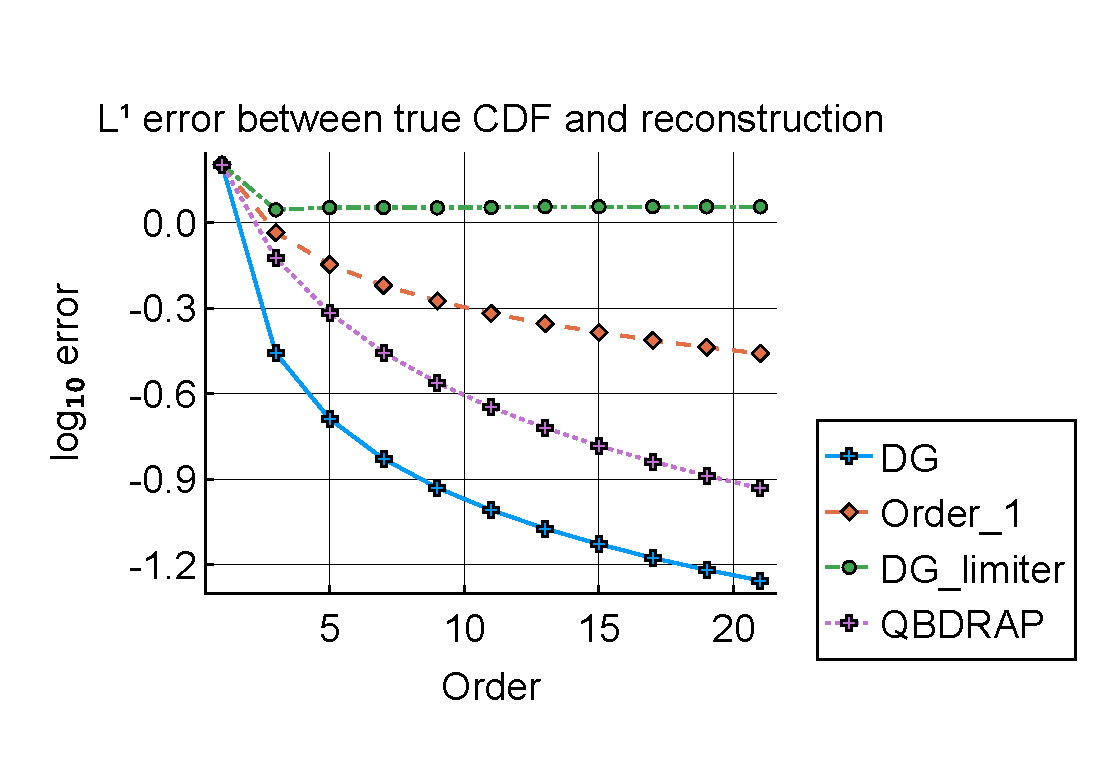
\includegraphics[width=0.5\textwidth,trim={0.75cm 0.8cm 0.25cm 1.25cm},clip]{chapter6/figs/wave/fun2/meshs_l1_cdf_error_formatted.pdf}%
	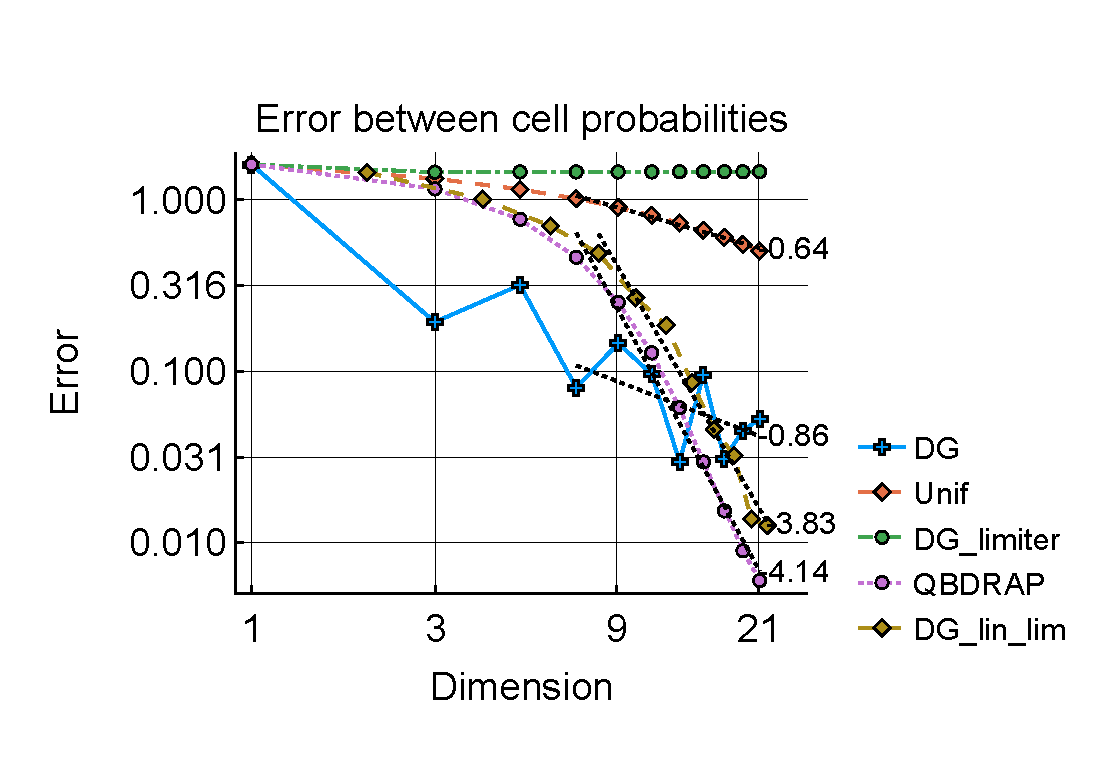
\includegraphics[width=0.5\textwidth,trim={0.75cm 0.8cm 0.25cm 1.25cm},clip]{chapter6/figs/wave/fun2/L1_cell_probs.pdf} 
	\caption{\(L^1\) error between the true CDF and the approximations (left) and the cell-wise error metric in (\ref{eqn: cell errors}) for the travelling wave problem in Example~\ref{ex: wave 2} where approximation were constructed via the DG method (blue solid line with crosses), DG method with the MUSCL limiter (green dash-dotted line with crosses), uniformisation method (orange dashed line with diamonds) and QBD-RAP method (purple dotted line with circles).} 
	\label{fig: fun 2 wave} 
\end{figure}
\exampleFloatBarrier
\end{example}

\begin{example}\label{ex: wave 6}
	Now consider an initial distribution which is truncated Gaussian with mean parameter 2.5 and standard deviation parameter 0.5, and truncated at the boundaries, 0 and 10;
	\begin{align}
		\mu([0,x)) := \mathbb P(X(0)\leq x, \varphi(0)=1)=\cfrac{\Phi((x-2.5)/0.5)1(0 \leq x < 10.0)}{\Phi(7.5/0.5)-\Phi(-2.5/0.5)} + 1(10\leq x), \label{eqn: kdjfksdf}
	\end{align}
	where \(\Phi(x)\) is the CDF of the standard normal distribution.

	At time \(t=4\) the distribution is truncated Gaussian with mean parameter 6.5, standard deviation parameter 0.5, and is truncated below at 4.0 and above at 10, and there is also a small mass at the upper boundary; 
	\begin{align}
		&\mathbb P(X(4)\leq x, \varphi(4)=1\mid X(0)\sim\mu, \varphi(0)=1)  
		=\cfrac{\Phi((x-6.5)/0.5)1(4.0\leq x)}{\Phi(7.5/0.5)-\Phi(-2.5/0.5)} + 1(10 \leq x).\label{eqn: bbbbbaabbaa}%\cfrac{\Phi(7.5/0.5)-\Phi(3.5/0.5)}{\Phi(7.5/0.5)-\Phi(-2.5/0.5)}.
	\end{align}
	At time \(t=4\) the mass at the boundary is approximately \(1.28\times 10^{-12}\) and there is a small discontinuity at \(x=4\) where the CDF jumps from \(0\) to \(\sim 2.87\times 10^{-7}\), due to the truncation of the initial distribution at \(0\). 

	Since the discontinuity at \(x=4\) is small (much smaller than numerical integration errors in the evaluation of the error metrics), and the distribution is otherwise smooth, we expect that the DG method will perform well for this example. Figures~\ref{fig: fun 6 wave cp} and~\ref{fig: fun 6 wave} confirms that this is indeed the case. For all three metrics the error obtained by the DG method rapidly decreases to a point where it is swamped by other numerical errors. This is characteristic of the DG method for the smooth problems we investigate throughout this chapter. For low order DG schemes there are regions where the approximated PDF is negative, however, as the order of the DG scheme increases, these regions disappear. Interestingly, even though this is a relatively smooth problem, the DG method with MUSCL limiter does not perform well. It must be that the initial and transient distributions are `sufficiently pointy' that oscillations in the numerical solutions occur and the limiter reduces the order of the scheme to linear. Both the uniformisation and QBD-RAP schemes perform similarly to previous examples. Comparing the cell-wise error plots in Figure~\ref{fig: fun 6 wave cp} with the higher-resolution error metrics in Figure~\ref{fig: fun 6 wave}, all the approximation schemes show a similar rate of decay of errors as a function of the dimension of the approximation. 
	\begin{figure}[h]
		\centering
		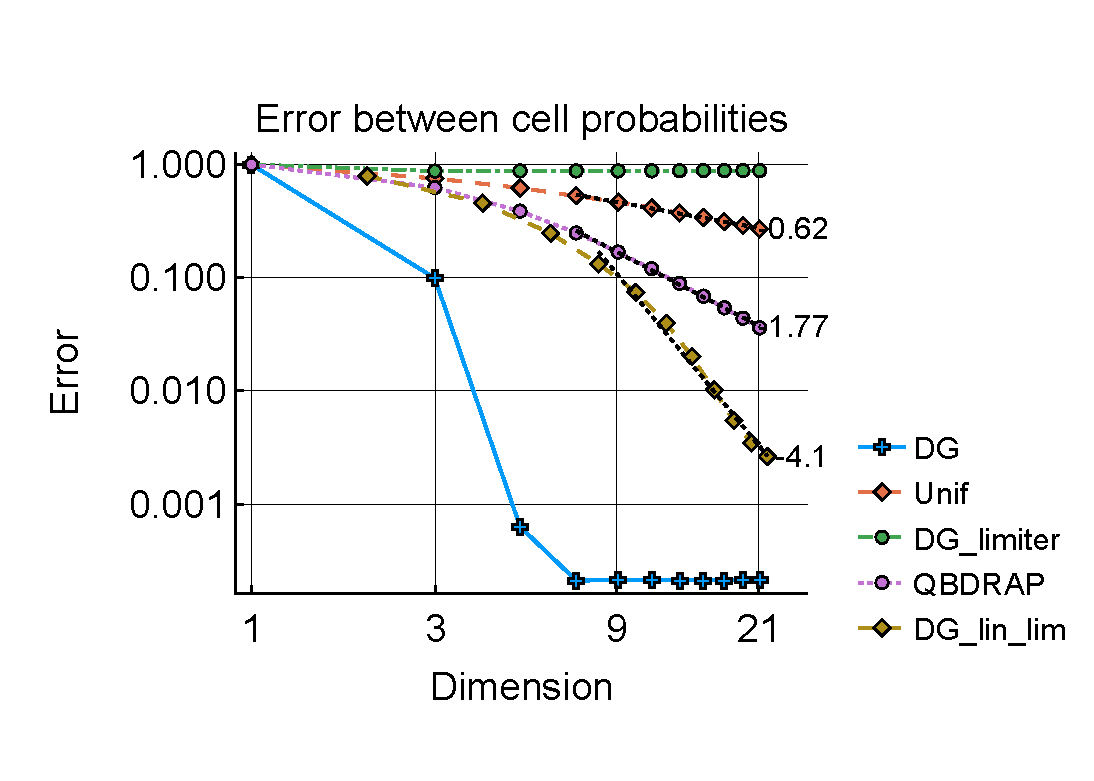
\includegraphics[width=0.5\textwidth,trim={0.75cm 0.8cm 0.25cm 1.25cm},clip]{chapter6/figs/wave/fun6/L1_cell_probs.pdf}
		\caption{Cell-wise error defined in (\ref{eqn: cell errors}) for the travelling wave problem in Example~\ref{ex: wave 6}. Plotted are the cell-wise errors for the DG method (blue solid line), DG method with Generalised MUSCL limiter (green dashed line), uniformisation method (orange dashed line) and QBD-RAP method (purple dotted line) versus the dimension of the approximation.}  
		\label{fig: fun 6 wave cp} 
	\end{figure}
	\begin{figure}[h]
		\centering
		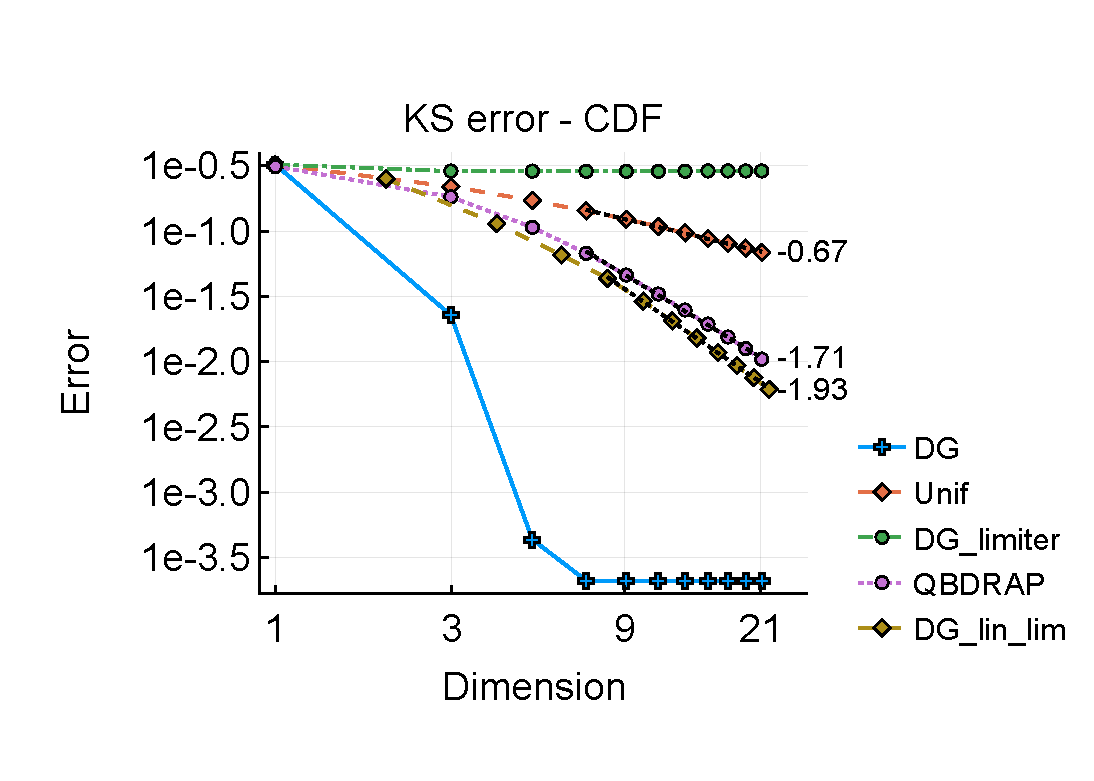
\includegraphics[width=0.5\textwidth,trim={0.75cm 0.8cm 0.25cm 1.25cm},clip]{chapter6/figs/wave/fun6/meshs_ks_error_formatted.pdf}%
		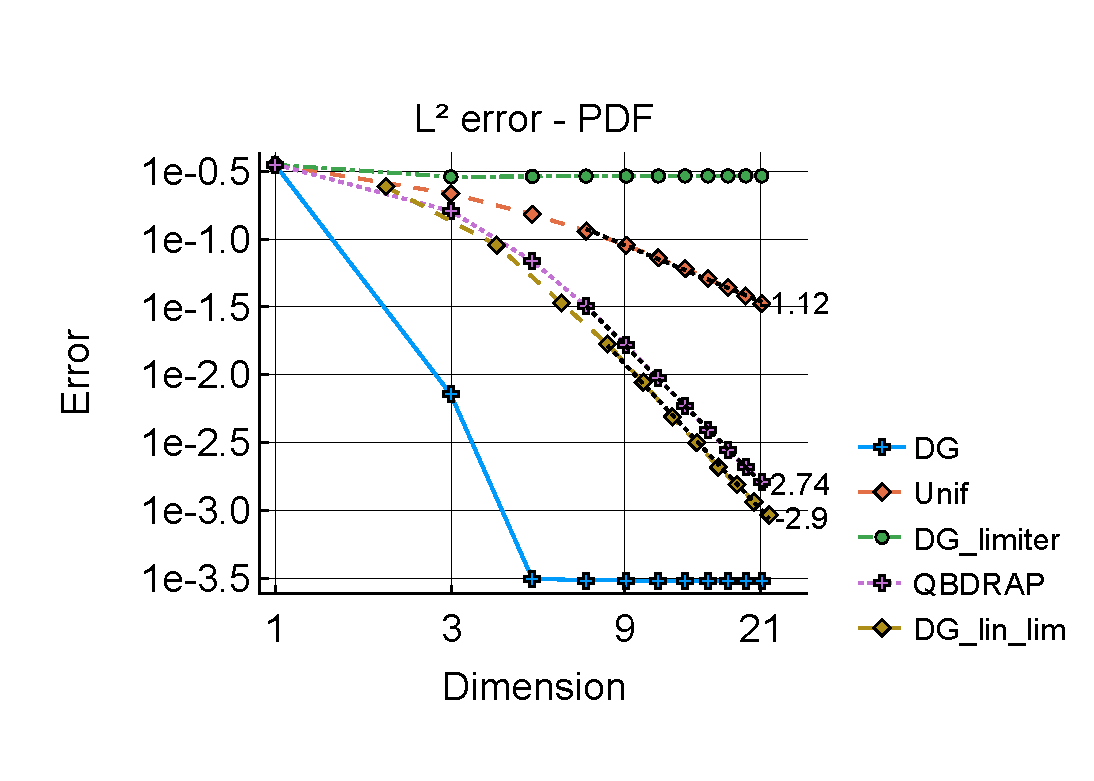
\includegraphics[width=0.5\textwidth,trim={0.75cm 0.8cm 0.25cm 1.25cm},clip]{chapter6/figs/wave/fun6/meshs_l2_pdf_error_formatted.pdf}
		\caption{KS error (left) and \(L^2\) error for the PDFs for Example~\ref{ex: wave 6} where approximations were constructed via the DG method (blue solid line with crosses), DG method with the MUSCL limiter (green dash-dotted line with crosses), uniformisation method (orange dashed line with diamonds) and QBD-RAP method (purple dotted line with circles).} 
		\label{fig: fun 6 wave} 
	\end{figure}
\exampleFloatBarrier
\end{example}

\begin{example}\label{ex: wave 1}
	We now want to look at how the methods might handle a mass at the boundary. We introduce an ephemeral second phase into the model with phase transition rate \(T_{22}=-1\), and fluid rate \(c_2=0\). The generator is therefore 
	\[T=\left[\begin{array}{cc} 0 & 0 \\ 1 & -1 \end{array}\right].\]

	We suppose that the initial condition is a point mass at the boundary in phase \(2\), i.e. \[\mathbb P(X(0)\leq x, \varphi(0)=2)=1(0\leq x).\] 
	With this initial condition, the transient distribution at time \(t=4\) is 
	\begin{align}
		&\mathbb P(X(4)\leq x,\varphi(4)=1 \mid X(0)=0,\varphi(0)=2) \nonumber 
		\\&= e^{T_{22}4}\left(e^{-T_{22}x}-1\right)1(4< x) + (1-e^{T_{22}4})1(4\geq x) \nonumber
		\\&= e^{-4}\left(e^{4x}-1\right)1(4< x) + (1-e^{-4})1(4\geq x) \label{eqn: asjda}
	\end{align}
	and 
	\begin{align}
		\mathbb P(X(4)\leq x,\varphi(4)=2 \mid X(0)=0,\varphi(0)=2) = e^{-4}1(0\leq x).
	\end{align}
	The PDF at \(t=4\) is discontinuous at \(x=4\), which is at the edge of a cell. For this problem, all methods can represent the initial condition exactly. 

	Figure~\ref{fig: fun 1 wave cp} plots the cell-wise error metric and Figure~\ref{fig: fun 1 wave} plots the KS error (right) and the \(L^2\) error between of the PDFs. Once again, the cell-wise error metrics in Figure~\ref{fig: fun 1 wave cp} show similar characteristics to the finer-resolution error metrics in Figure~\ref{fig: fun 1 wave}. Observing Figures~\ref{fig: fun 1 wave cp} and \ref{fig: fun 1 wave}, the DG method with MUSCL limiter does not perform well, which might be expected due to the discontinuity in the transient distribution at \(x=4\) in Phase~1. The uniformisation and QBD-RAP methods appear to converge, with the QBD-RAP method converging faster. The DG method converges fastest, however, produces approximations with negative and oscillatory solutions as we might expect given the discontinuity. A selection of approximations to the transient PDF are shown in Figure~\ref{fig: pdf wave fun 1}.
	\begin{figure}[h]
		\centering
		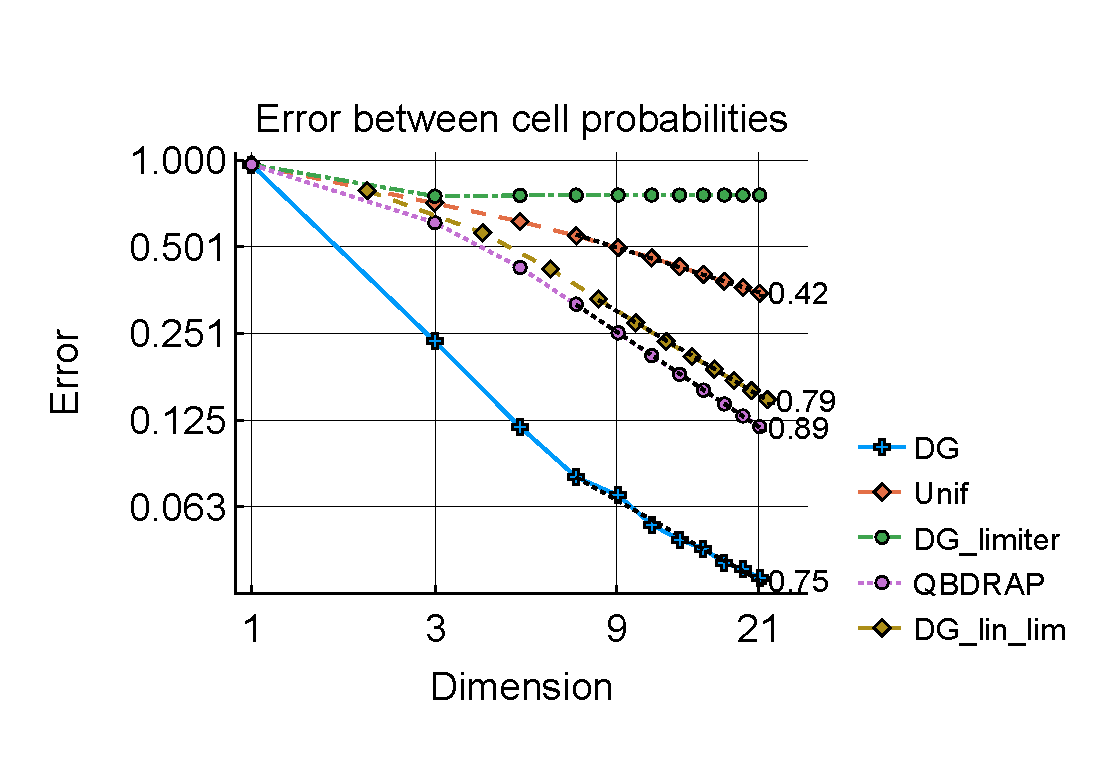
\includegraphics[width=0.5\textwidth,trim={0.75cm 0.8cm 0.25cm 1.25cm},clip]{chapter6/figs/wave/fun1/L1_cell_probs.pdf} 
		\caption{Cell-wise error for the travelling wave problem in Example~\ref{ex: wave 1}. Plotted are the cell-wise errors for the DG method (blue solid line), DG method with Generalised MUSCL limiter (green dashed line), uniformisation method (orange dashed line) and QBD-RAP method (purple dotted line) versus the dimension of the approximation.}  
		\label{fig: fun 1 wave cp} 
	\end{figure}
	\begin{figure}[h]
		\centering
		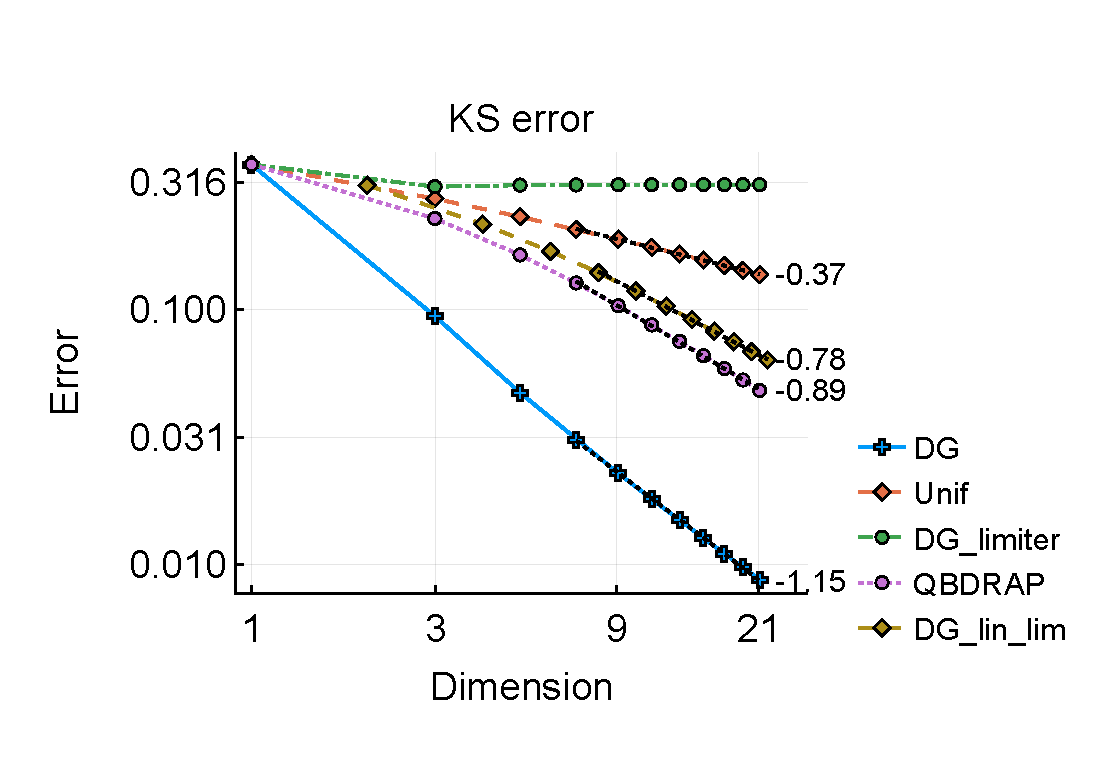
\includegraphics[width=0.5\textwidth,trim={0.75cm 0.8cm 0.25cm 1.25cm},clip]{chapter6/figs/wave/fun1/meshs_ks_error_formatted.pdf}%
		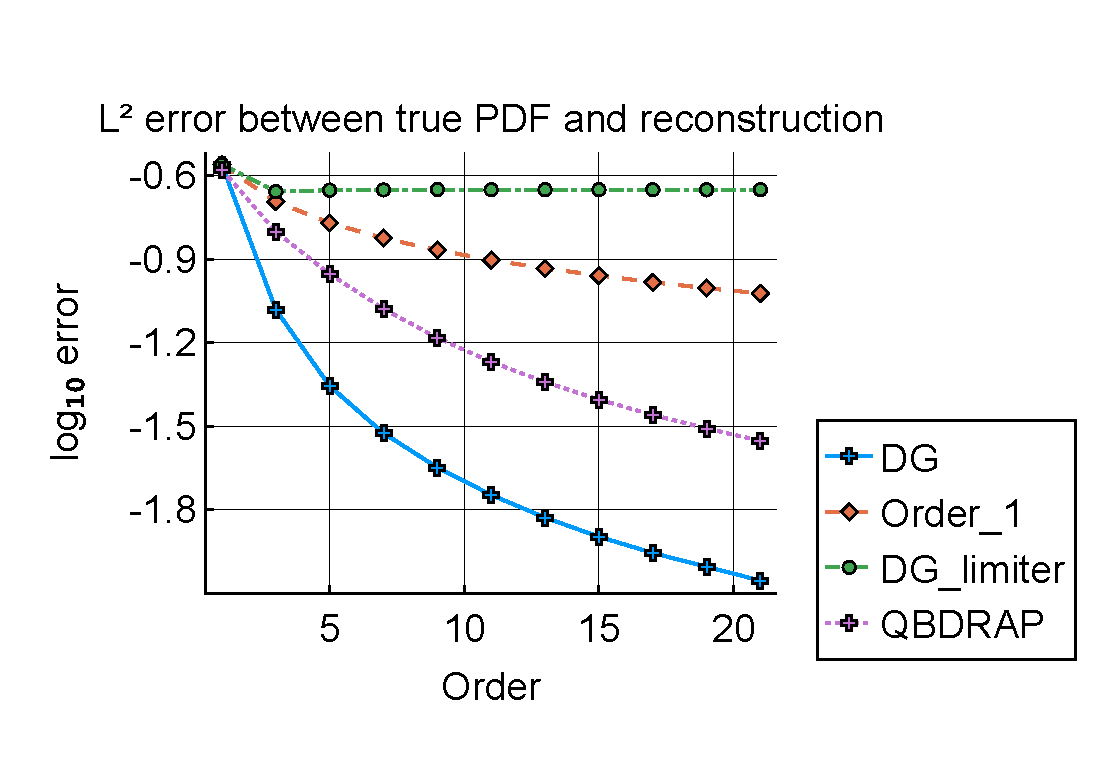
\includegraphics[width=0.5\textwidth,trim={0.75cm 0.8cm 0.25cm 1.25cm},clip]{chapter6/figs/wave/fun1/meshs_l2_pdf_error_formatted.pdf}
		\caption{KS error (left) and \(L^2\) error of the PDFs for the travelling wave problem in Example~\ref{ex: wave 1} where approximations were constructed via the DG method (blue solid line with crosses), DG method with the MUSCL limiter (green dash-dotted line with crosses), uniformisation method (orange dashed line with diamonds) and QBD-RAP method (purple dotted line with circles).} 
		\label{fig: fun 1 wave} 
	\end{figure}
	\begin{figure}[h]
		\centering
		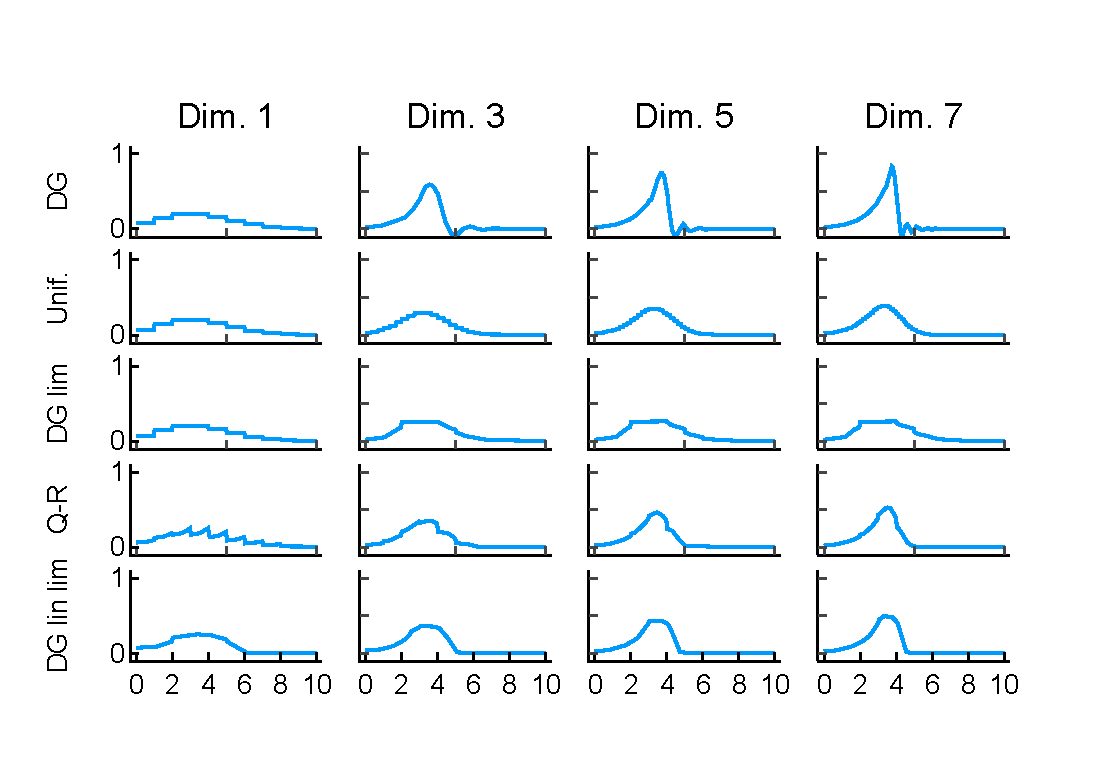
\includegraphics[width=\textwidth,trim={0cm 1.25cm 0cm 1.25cm},clip]{chapter6/figs/wave/fun1/pdf_formatted.pdf}
		\caption{Approximate PDFs for Example~\ref{ex: wave 1} using the DG (top row), uniformisation (second row), DG with MUSCL limiter (third row) and QBD-RAP (bottom row) methods, with dimensions 1, 3, 5, and 7 (columns). The true density function is \(e^{-4}e^{x}1(x<4)\).} 
		\label{fig: pdf wave fun 1}
	\end{figure} 
	\exampleFloatBarrier
\end{example} 

\FloatBarrier
\section{Stationary distributions} \label{sec:stat}
We briefly turn our attention to stationary distributions of fluid queues. Since the stationary distribution is smooth we expect that the DG method will work well here. The stationary distribution is convenient as we can evaluate them analytically \cite{s2017} and do not require us to approximate initial conditions or integrate over time. Hence, analysing the performance of the approximation methods with the stationary distribution allows us to instrument the ability of the methods to capture the stochastic dynamics, without numerical integration in time.

Here we analyse a simple model which is based on Example~2 in \citep{bean2009}, except here we add a lower boundary to the model (no lower boundary is specified in Example~2 of \citep{bean2009} as it is inconsequential to their analysis). 

% \begin{model}\label{model: simple}
% 	Consider a fluid queue where the driving process is a CTMC with state space \(\calS=\{1,2,3,4\}\), generator 
% 	\[\bs T = \left[\begin{array}{cccc}
% 		-1.1 & 1.1 & 0 & 0 \\
% 		1 & -1 & 0 & 0 \\ 
% 		0.01 & 0 & -0.01 & 0 \\
% 		0 & 0.01 & 0 & -0.01 
% 	\end{array}\right],\]
% 	and there are associated rates \(c_1=1, c_2 = -1, c_3=0, c_4=0\) and boundaries at \(x=0\) and \(x=10\). We specify two types of behaviour at the boundary.
% 	\begin{enumerate}[a)]
% 		\item (Absorbing model) Upon hitting the lower boundary, the process transitions from phase \(2\) to phase \(j\) with probability \(p_{2j}\) where 
% 		\[\vligne{p_{21} & p_{22} & p_{23} & p_{24}} = \vligne{0 & 0 & 1 & 0}.\]
% 		Upon hitting the upper boundary, the process transitions from phase \(1\) to phase \(j\) with probability \(p_{1j}\) where 
% 		\[\vligne{p_{11} & p_{12} & p_{13} & p_{14}} = \vligne{0 & 0 & 0 & 1}.\]
% 		\item (Reflecting model) Upon hitting the lower boundary, the process transitions from phase \(2\) to phase \(j\) with probability \(p_{2j}\) where 
% 		\[\vligne{p_{21} & p_{22} & p_{23} & p_{24}} = \vligne{1 & 0 & 0 & 0}.\]
% 		Upon hitting the upper boundary, the process transitions from phase \(1\) to phase \(j\) with probability \(p_{1j}\) where 
% 		\[\vligne{p_{11} & p_{12} & p_{13} & p_{14}} = \vligne{0 & 1 & 0 & 0}.\]
% 	\end{enumerate}
% \end{model}
% Phases~3 and 4 are included only to capture behaviour at the boundary.

% For Model~\ref{model: simple}~a), upon hitting the boundary, the process stays at the boundary for an exponentially distributed amount of time with mean 100. For Model~\ref{model: simple}~b), upon hitting the boundary, the process is immediately reflected. In Model~\ref{model: simple}~b) phases 3 and 4 are ephemeral and are included only for notational convenience. 


\begin{model}\label{model: simple}
	Consider a fluid queue where the driving process is a CTMC with state space \(\calS=\{1,2,3,4\}\), generator 
	\[\bs T = \left[\begin{array}{cccc}
		-1.1 & 1.1 \\
		1 & -1 \\ 
	\end{array}\right],\]
	and there are associated rates \(c_1=1, c_2 = -1,\) and boundaries at \(x=0\) and \(x=10\). We specify two types of behaviour at the boundary.
	
	Upon hitting the lower boundary, the process transitions from phase \(2\) to phase \(j\) with probability \(p_{2j}\) where 
		\[\vligne{p_{21} & p_{22} } = \vligne{1 & 0}.\]
		Upon hitting the upper boundary, the process transitions from phase \(1\) to phase \(j\) with probability \(p_{1j}\) where 
		\[\vligne{p_{11} & p_{12} } = \vligne{0 & 1}.\]
	Thus, upon hitting the boundary, the fluid queue immediately transitions to the other phase and is reflected.
\end{model}

The model was discretised using the DG, uniformisation and QBD-RAP methods using ten cells of width \(1\). We compute the coefficients for the stationary distribution in the following way. Suppose that a given discretisation method results in an approximation to the generator of the fluid queue as a matrix \(\bs B\). Then the stationary coefficients are found by solving 
\begin{align}
	\bs b \bs B = 0,\\
	\mbox{such that } \bs b\bs 1=1,
\end{align}
for the coefficients \(\bs b\). 

% \paragraph{Model~\ref{model: simple}~a) Absorbing model}
% Figure~\ref{fig: absorbing stationary} plots KS errors between the true stationary CDF and the approximations (left) and the \(L^2\) error between the true stationary PDF and the approximations. Clearly the DG method is superior here as its error rapidly decreases to a point where is become insignificant compared to other numerical errors. The QBD-RAP method and uniformisation method both appear to be converging, with the errors for the QBD-RAP method decreasing faster.
% \begin{figure}[h]
% 	\centering
% 	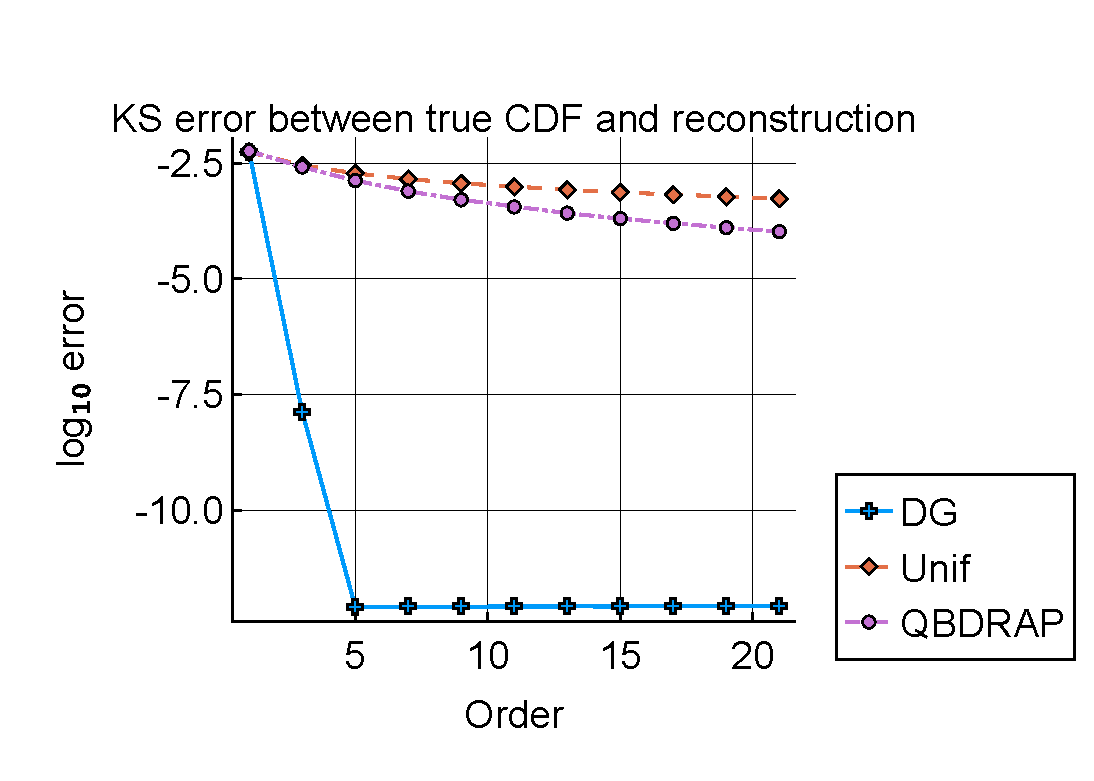
\includegraphics[width=0.5\textwidth,trim={0.75cm 0.8cm 0.25cm 1.25cm},clip]{chapter6/figs/hitting_times_model/absorbing_model/stationary_distribution/ks_error_formatted.pdf}%
% 	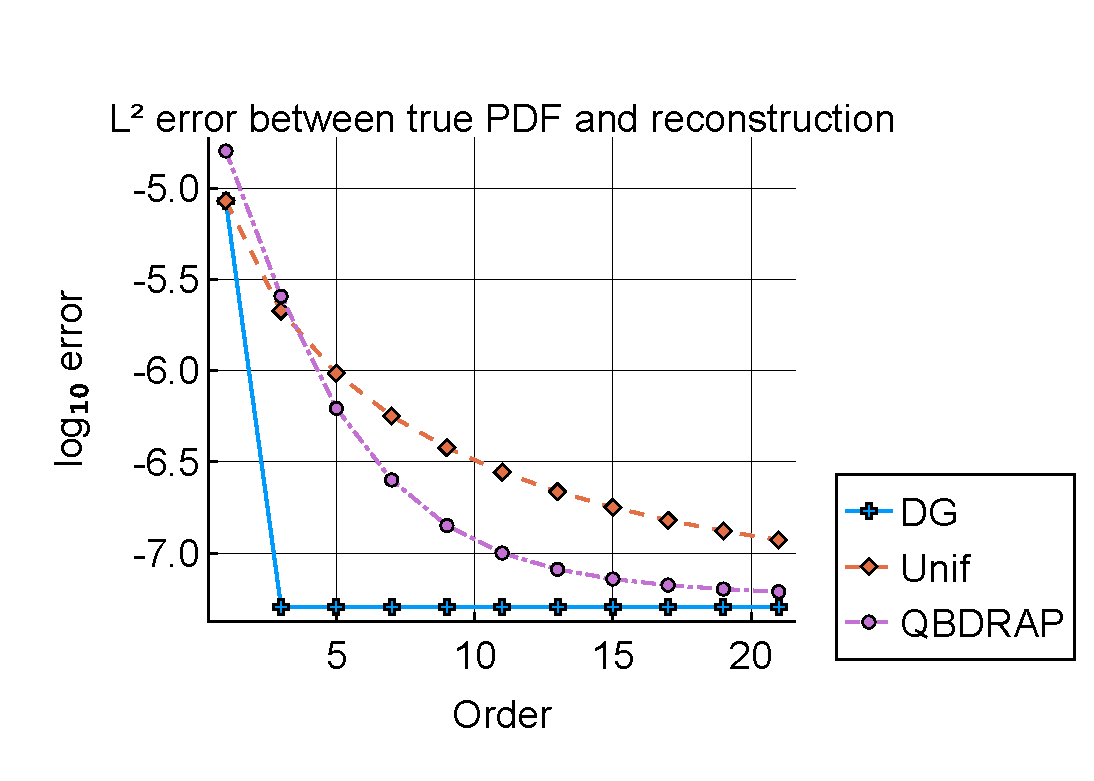
\includegraphics[width=0.5\textwidth,trim={0.75cm 0.8cm 0.25cm 1.25cm},clip]{chapter6/figs/hitting_times_model/absorbing_model/stationary_distribution/l2_pdf_error_formatted.pdf}
% 	\caption{KS error between the true stationary CDF  and the approximations (left) and \(L^2\) error between the true stationary PDF and the approximations for Model~\ref{model: simple}~a) using the DG method (blue solid line with crosses), uniformisation method (orange dashed line with diamonds) and QBD-RAP method (green dash-dotted line with circles).} 
% 	\label{fig: absorbing stationary} 
% \end{figure}

\paragraph{Model~\ref{model: simple}.}
Figure~\ref{fig: reflecting stationary} plots KS errors between the true stationary CDF and the approximations (left) and the \(L^2\) error between the true stationary PDF and the approximations. Clearly the DG method is superior here as its error rapidly decreases to a point where is become insignificant compared to other numerical errors. The QBD-RAP method and uniformisation method both appear to be converging, with the errors for the QBD-RAP method decreasing faster.
\begin{figure}[h]
	\centering
	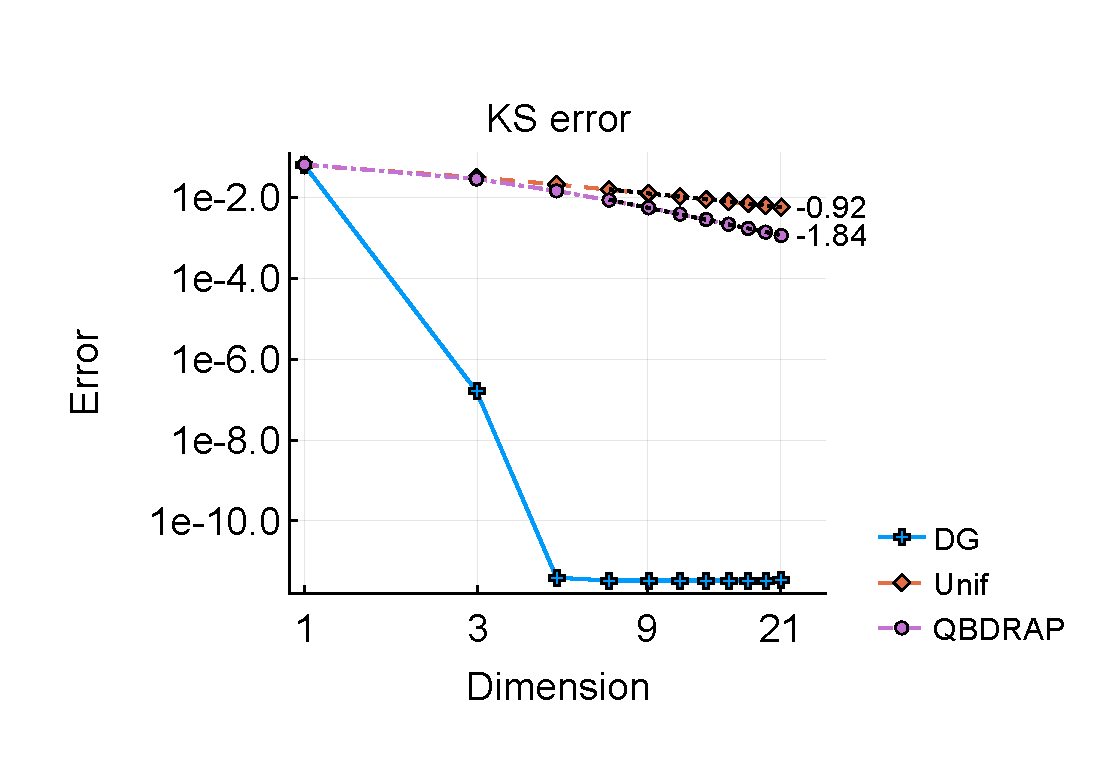
\includegraphics[width=0.5\textwidth,trim={0.75cm 0.8cm 0.25cm 1.25cm},clip]{chapter6/figs/hitting_times_model/reflecting_model/stationary_distribution/ks_error_formatted.pdf}%
	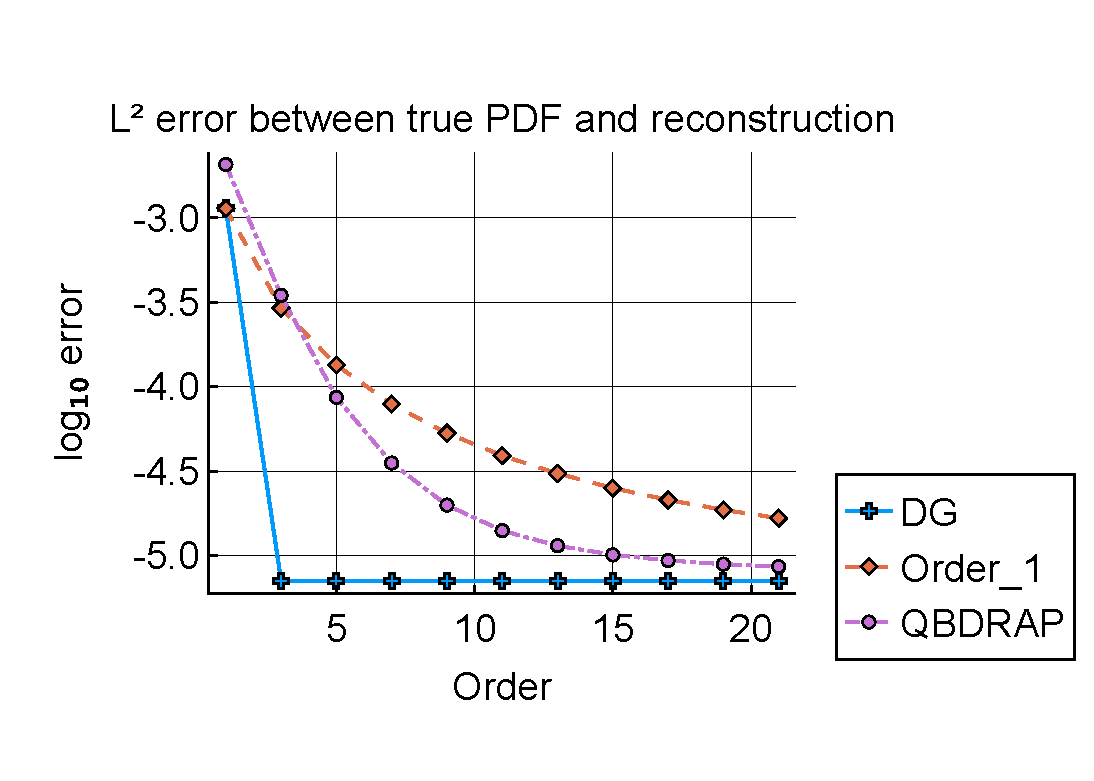
\includegraphics[width=0.5\textwidth,trim={0.75cm 0.8cm 0.25cm 1.25cm},clip]{chapter6/figs/hitting_times_model/reflecting_model/stationary_distribution/l2_pdf_error_formatted.pdf}
	\caption{KS error (left) and \(L^2\) error of the PDFs for Model~\ref{model: simple} using the DG method (blue solid line with crosses), uniformisation method (orange dashed line with diamonds) and QBD-RAP method (purple dotted line with circles).} 
	\label{fig: reflecting stationary} 
\end{figure}

\FloatBarrier
\section{Transient distributions}\label{sec: transient approx}
Once again we consider Model~\ref{model: simple} and use the same spatial discretisation as described in Section~\ref{sec:stat} (ten cells with width \(\Delta=1\)). Two initial conditions are considered, a point mass at 0 in phase 1, and the initial distribution with PDF 
\begin{align}
	\cfrac{1}{2}e^{-x}/(1-e^{-10})\label{eqn: exp init cond}
\end{align}
in phases 1 and 2, with no mass at the boundaries. We numerically integrate over time until time \(t=2.0\) using the SSPRK4 method with t-step size 0.005.\footnote{Once again, the \(t\)-step size must be chosen to ensure that numerical integration over time is stable up to dimension 21, adhering to a CFL-like condition \cite[Section~4.8]{nodalDGBook}.} We apply the DG method with, and without, the Generalised MUSCL slope limiter. 

To obtain a \emph{ground truth} 5,000,000 realisations of the fluid queue were simulated until \(t=2\), then the empirical CDF and the masses within each cell and at the boundaries were computed from the simulations. We do not attempt to numerically approximate the true PDF via simulation. We then compute the KS and \(L^1\) error metrics between the approximated CDF and simulated CDF, as well as the cell-wise error metric, given as follows. 
\begin{align}
	&\sum_{j\in\{1,2\}}\sum_{\ell=1}^{10} \left|\mathbb P_{sim}(X(2)\in\calD_{\ell,j}, \varphi(2)=j\mid X(0)=0.5,\varphi(0)=1)-p(2,\ell,j)\right|\nonumber 
	\\&+\left|\mathbb P_{sim}(X(2)\in\{10\}, \varphi(2)=4\mid X(0),\varphi(0))-p(2,11,4)\right|\nonumber 
	\\&+\left|\mathbb P_{sim}X(2)\in\{0\}, \varphi(2)=3\mid X(0),\varphi(0))-p(2,0,3)\right| \label{eqn: cell errors 2}
\end{align}
where \(p(2,\ell,j)\) is an approximation to \(\mathbb P_{sim}(X(2)\in\calD_{\ell,j}, \varphi(2)=j\mid X(0),\varphi(0))\), \(p(2,11,4)\) is an approximation to \(\mathbb P_{sim}(X(2)\in\{10\}, \varphi(2)=4\mid X(0),\varphi(0))\), and \(p(2,0,3)\) is an approximation to \(\mathbb P_{sim}(X(2)\in\{10\}, \varphi(2)=3\mid X(0),\varphi(0))\), and \(\mathbb P_{sim}\) denotes an empirical probability evaluated using the simulations of the fluid queue. 

To account for possible Monte-Carlo error, we used a bootstrap with 1,000 bootstrap samples. We sample 5,000,000 realisations of the fluid queue with replacement from the original 5,000,000 samples, then compute error metrics with the resampled data. We resample 1,000 times. Via the bootstrap, we report the \(5\)th and \(95\)th percentile of the sampling distribution of the errors. 

To evaluate error metrics, we use a grid of 10,001 evenly spaced points for each phase.

To approximate the point mass initial condition we compute the initial coefficients for each scheme exactly. For the exponential initial condition in (\ref{eqn: exp init cond}) we compute the initial coefficients via Gauss-Lobatto quadrature for the DG method, by using the mid-point rule for the uniformisation method, and by using a trapezoidal rule with 2,001 points on each cell for the QBD-RAP method. 

\paragraph{Model~\ref{model: simple} with exponential initial condition}
Figure~\ref{fig: reflecting transient exp} shows the error metrics for the four different spatial discretisation schemes (DG, DG with MUSCL limiter, uniformisation and QBD-RAP). For both error metrics the DG scheme converges rapidly until computational errors become significant. The uniformisation and QBD-RAP schemes converge at a slower rate than the DG method, with the QBD-RAP scheme converging faster than the uniformisation method. The DG scheme with MUSCL limiter does not appear to be converging, which suggests there is at least one iteration during the numerical integration over time at which the numerical solution displays oscillations. However, when the DG approximations for the distribution at time \(t=2\) are plotted, they do not display oscillations (not shown). This suggests that the oscillations which might occur with the DG scheme must be transient, and have dissipated by time \(t=2\). The oscillations which the limiter detects in the DG scheme are likely from the reflecting boundary at \(x=0\). In the early stages of the evolution of the model the majority of the density in Phase~2 near zero will move to the left at rate 1 and hit the boundary at \(x=0\). Upon hitting the boundary, the density is reflected into Phase~1. Meanwhile, the initial density in Phase~1 moves to the right at rate 1 and the density reflected at the boundary from Phase~2 fills in to the region between \(x=0\) and \(x=t\) in Phase~1. Intuitively, in the early evolution of the model, there will be a sharp peak in the transient density at \(x=t\) -- I suspect that the transient density is continuous at this point, but not differentiable.  %
\begin{figure}[h]
	\centering
	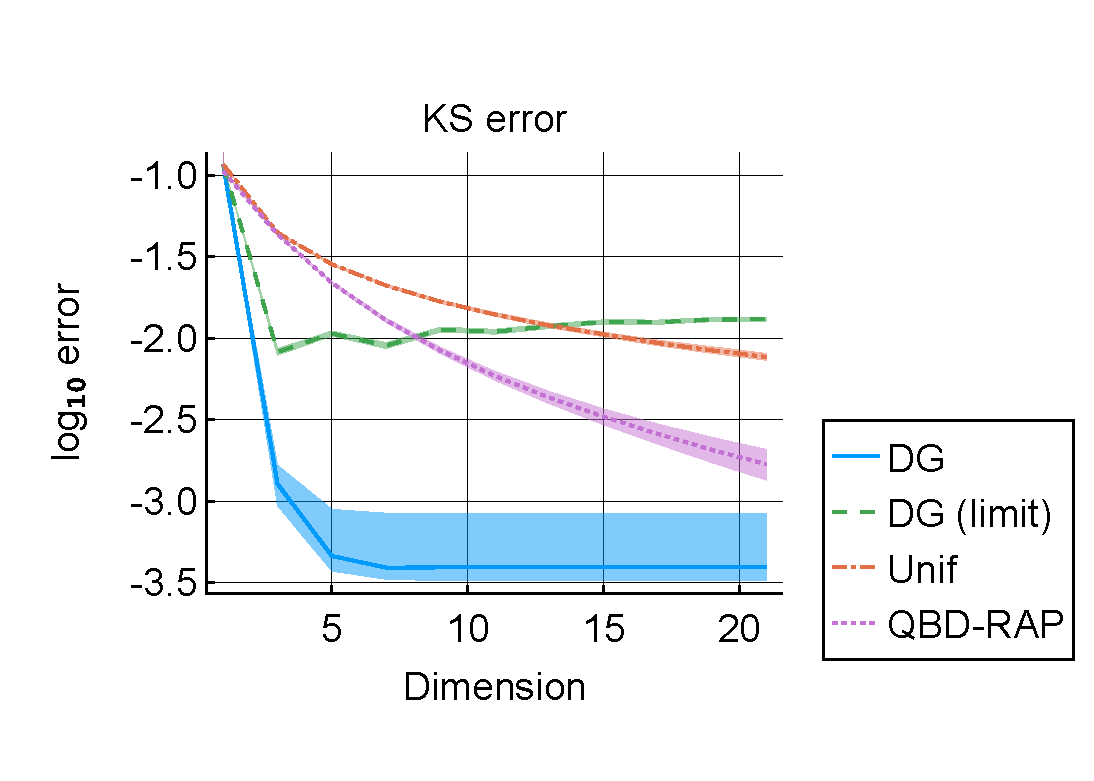
\includegraphics[width=0.5\textwidth,trim={0.75cm 0.8cm 0.25cm 1.25cm},clip]{chapter6/figs/hitting_times_model/reflecting_model/transient_distribution/exp/ks_error_formatted.pdf}%
	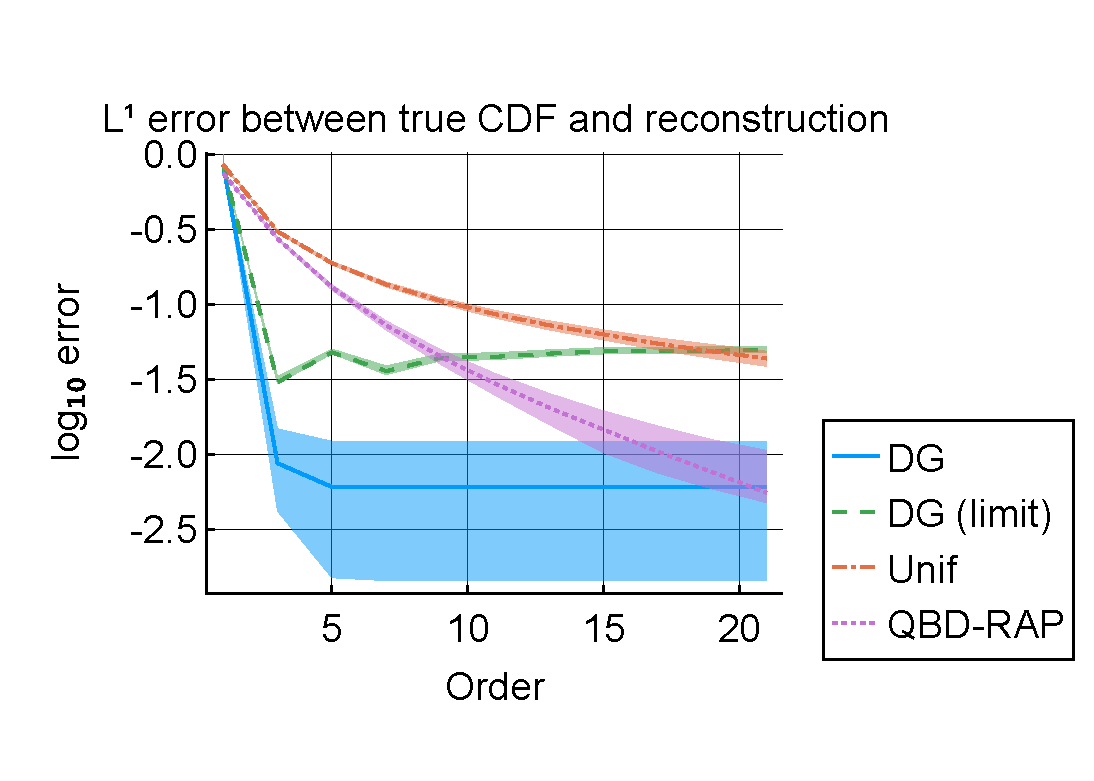
\includegraphics[width=0.5\textwidth,trim={0.75cm 0.8cm 0.25cm 1.25cm},clip]{chapter6/figs/hitting_times_model/reflecting_model/transient_distribution/exp/l1_cdf_error_formatted.pdf}
	\caption{KS (left) and \(L^1\) (right) errors between the true transient CDF at time \(t=2\) for Model~\ref{model: simple} with the exponential initial condition, where the approximations were obtained via the DG method (blue solid line), DG method with Generalised MUSCL limiter (green dashed line), uniformisation method (orange dashed line) and QBD-RAP method (purple dotted line). Bootstrapped 90\% confidence intervals are shown by the lighter coloured bars surrounding the lines.} 
	\label{fig: reflecting transient exp} 
\end{figure}

Figure~\ref{fig: reflecting transient exp cp} plots the cell-wise error metric (\ref{eqn: cell errors 2}) for Model~\ref{model: simple} with the exponential initial condition. Since the cell-wise errors do not require us to reconstruct the value of the solution within each cell, then this metric allows us to observe the error characteristics of the methods without reconstruction. Figure~\ref{fig: reflecting transient exp cp} shows similar convergence characteristics to the other error metrics in Figure~\ref{fig: reflecting transient exp}. 
\begin{figure}[h]
	\centering
	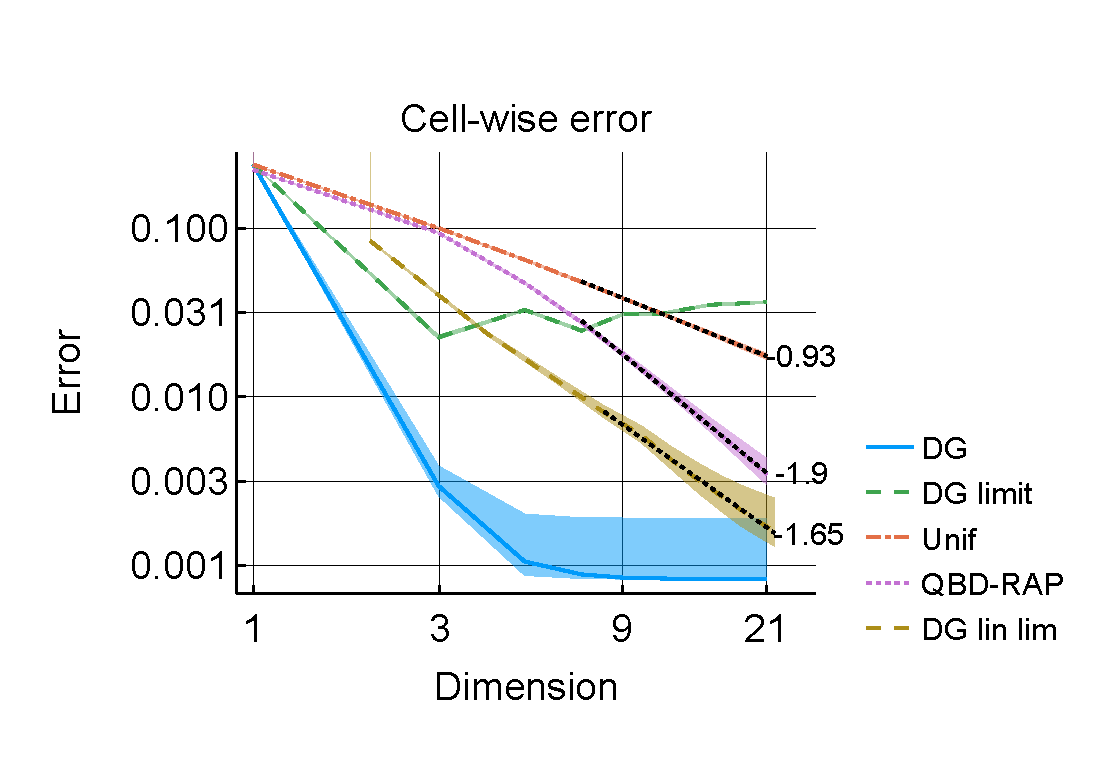
\includegraphics[width=0.5\textwidth,trim={0.75cm 0.8cm 0.25cm 1.25cm},clip]{chapter6/figs/hitting_times_model/reflecting_model/transient_distribution/exp/L1_cell_probs_error_formatted.pdf}
	\caption{Cell-wise error metric from (\ref{eqn: cell errors 2}) for Model~\ref{model: simple} with the exponential initial condition, where the approximations were obtained via the DG method (blue solid line), DG method with Generalised MUSCL limiter (green dashed line), uniformisation method (orange dashed line) and QBD-RAP method (purple dotted line). Bootstrapped 90\% confidence intervals are shown by the lighter coloured bars surrounding the lines.} 
	\label{fig: reflecting transient exp cp} 
\end{figure}
\exampleFloatBarrier
\paragraph{Model~\ref{model: simple} with a point-mass initial condition}
Figure~\ref{fig: reflecting transient pm} shows the error metrics for the four different spatial discretisation schemes (DG, DG with MUSCL limiter, uniformisation and QBD-RAP). Comparing the error metrics in Figure~\ref{fig: reflecting transient pm} for the point mass initial condition with the ones in Figure~\ref{fig: reflecting transient exp} for the exponential initial condition all schemes perform worse for the point mass initial condition. Regarding comparative rates of convergence for this problem, the DG scheme converges fastest, followed by the QBD-RAP scheme, then the uniformisation scheme, while the DG scheme with MUSCL limiter does not appear to converge due to the limiter reducing the scheme to a linear approximation around the discontinuity. %
\begin{figure}[h]
	\centering
	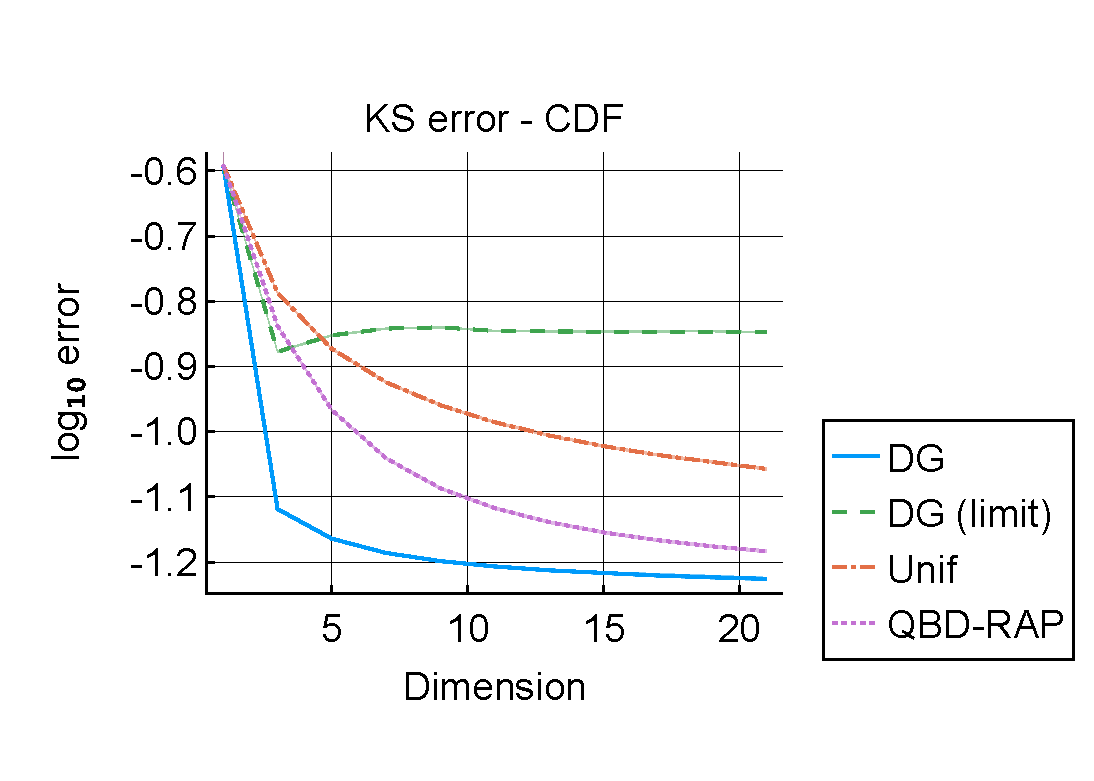
\includegraphics[width=0.5\textwidth,trim={0.75cm 0.8cm 0.25cm 1.25cm},clip]{chapter6/figs/hitting_times_model/reflecting_model/transient_distribution/point_mass/ks_error_formatted.pdf}%
	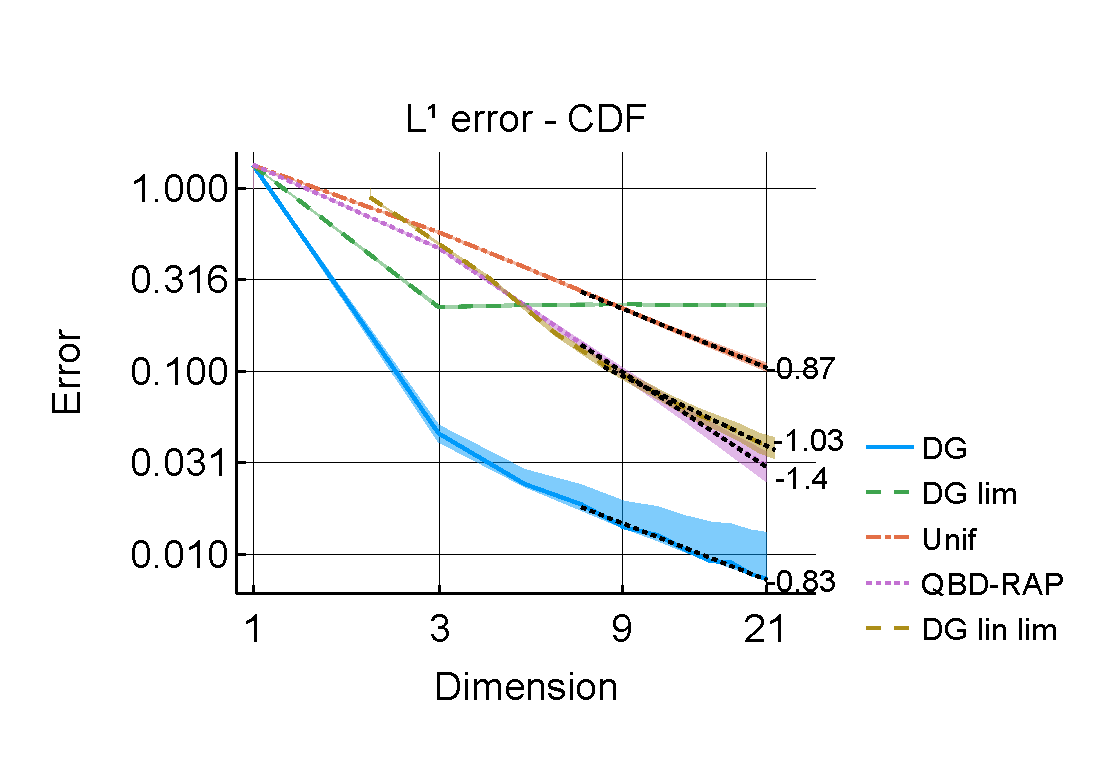
\includegraphics[width=0.5\textwidth,trim={0.75cm 0.8cm 0.25cm 1.25cm},clip]{chapter6/figs/hitting_times_model/reflecting_model/transient_distribution/point_mass/l1_cdf_error_formatted.pdf}
	\caption{KS (left) and \(L^1\) errors between of the CDF (right) at time \(t=2\) for Model~\ref{model: simple} with the point-mass initial condition, where the approximations were obtained via the DG method (blue solid line), DG method with Generalised MUSCL limiter (green dashed line), uniformisation method (orange dashed line) and QBD-RAP method (purple dotted line). Bootstrapped 90\% confidence intervals are shown by the lighter coloured bars surrounding the lines.} 
	\label{fig: reflecting transient pm} 
\end{figure}

Figure~\ref{fig: reflecting transient pm cp} plots the cell-wise error metric (\ref{eqn: cell errors 2}) for Model~\ref{model: simple} with the point mass initial condition. Figure~\ref{fig: reflecting transient pm cp} suggests that approximating the cell-wise error seems to be a difficult problem. This is likely caused by the discontinuity at \(x=2\) in phase \(1\), which lies exactly on a cell boundary. To investigate how the position of the discontinuity might affect the error metrics we evolved the model to time \(t=2.1\) and computed the KS error, \(L^1\) error between the CDFs and the cell-wise error. Once again, we use simulation and bootstrapping to approximate the \emph{ground truth}. The plots (not shown) of KS error and \(L^1\) error between the CDFs for the model at times \(t=2\) and \(t=2.1\) are relatively similar and not noteworthy. The plot of the cell-wise error metric at time \(t=2.1\) in Figure~\ref{fig: reflecting transient pm t2.1} is somewhat more interesting. Figure~\ref{fig: reflecting transient pm t2.1} shows that the cell-wise error metric is somewhat volatile for the DG scheme; I suspect that this is due to the oscillations in the DG approximation. In contrast, in Figure~\ref{fig: reflecting transient pm t2.1} the uniformisation and QBD-RAP schemes have monotonically decreasing error curves.
\begin{figure}[h]
	\centering
	\includegraphics[width=0.5\textwidth,trim={0.75cm 0.8cm 0.25cm 1.25cm},clip]{chapter6/figs/hitting_times_model/reflecting_model/transient_distribution/point_mass/L1_cell_probs_error_formatted.pdf}
	\caption{Cell-wise errors for Model~\ref{model: simple} at time \(t=2\) with the point mass initial condition, where the approximations were obtained via the DG method (blue solid line), DG method with Generalised MUSCL limiter (green dashed line), uniformisation method (orange dashed line) and QBD-RAP method (purple dotted line). Bootstrapped 90\% confidence intervals are shown by the lighter coloured bars surrounding the lines.} 
	\label{fig: reflecting transient pm cp} 
\end{figure}%
\begin{figure}[h]
	\centering
	\includegraphics[width=0.5\textwidth,trim={0.75cm 0.8cm 0.25cm 1.25cm},clip]{chapter6/figs/hitting_times_model/reflecting_model/transient_distribution/point_mas_t_2.1/L1_cell_probs_error_formatted.pdf}
	\caption{\(L^1\) errors between the simulated and approximated cell masses for Model~\ref{model: simple} at time \(t=2.1\) with the point mass initial condition, and the corresponding approximations obtained via the DG method (blue solid line), DG method with Generalised MUSCL limiter (green dashed line), uniformisation method (orange dashed line) and QBD-RAP method (purple dotted line). Bootstrapped 90\% confidence intervals are shown by the lighter coloured bars surrounding the lines.} 
	\label{fig: reflecting transient pm t2.1} 
\end{figure}

\FloatBarrier
\section{Hitting times}\label{sec: return approx}
Once again we consider Model~\ref{model: simple}. Let \(\zeta_{X}(\{0,1\}) = \{\inf t>0 \mid X(t)=0, \mbox{ or }X(t)=1\},\) be the first hitting time of \(\{X(t)\}\) on the set \(\{0,1\}\). The distribution of the hitting time in phase \(i\in\{1,2\}\) is 
\begin{equation}\label{eqn: hit cdf}\mathbb P(\zeta_{X}(\{0,1\}) < t, \varphi(t)=i\mid \bs X(0)\sim \mu),\end{equation}
for some initial distribution \(\mu\). We look at two initial conditions; an exponential with equal mass in each phase, 
\[\mathbb P(X(0)\in\wrt x,\varphi(0)=i) = e^{-x}/(1-e^{-1})/2,\,i\in\{1,2\},\]
and a point mass at \(X(0)=0\) in phase \(\varphi(0)=1\). 

We use the DG, uniformisation and QBD-RAP methods to discretise the fluid queue and partition \([0,1]\) into three intervals of width \(1/3\). To capture the mass which has left the interval \([0,1]\), we suppose that when the process hits the boundary it is absorbed forever at the boundary and in the phase in which the process first hit the boundary. 

We integrate the schemes until time \(t=10\) using the SSPRK4 method with \(t\)-step size 0.005/3.\footnote{Since we use a smaller cell-width in this example than in previous examples we need to reduce the \(t\)-step size accordingly to ensure that numerical integration is stable for schemes up to dimension 21, adhering to a CFL-like condition \cite[Section~4.8]{nodalDGBook}.} We use the DG scheme with and without a slope limiter during the time-integration. At each time-step of the numerical integration, we record the amount of mass at the absorbing boundaries in each phase, which gives us an approximation of the cumulative distribution function of the hitting time in each phase up to time \(t=10\). 

As a \emph{ground truth} we simulated 5,000,000 realisations and recorded the hitting time on the boundary of the interval \([0,1]\) and the phase at the time of hitting. We then compute the empirical CDF of the hitting probabilities 
\[\mathbb P(\zeta_{X}(\{0,1\}) < t, \varphi(t)=i\mid \bs X(0)\sim \mu),\] 
for \(t=0.005/3\times k\), \(k=0,...,6000\). 

To account for Monte-Carlo errors we took 1,000 bootstrap resamples of the original 5,000,000 samples and computed the empirical CDF of the hitting probabilities for each bootstrap sample. For each bootstrap sample, we resampled 5,000,000 points with replacement from the original 5,000,000 realisations. For each bootstrap sample we computed the error metrics between the empirical and approximated CDFs and recorded the 5th and 95th percentile of the distribution of the errors. 

\paragraph{Exponential initial condition}
Figure~\ref{fig: hitting time exp} shows the error metrics recorded for the four different numerical approximation schemes. The uniformisation and QBD-RAP method both appear to converge, with the QBD-RAP converging at a faster rate. For both error metrics the DG scheme performs the best. For the \(L^1\) error metric the DG scheme converges up to order 5 after which there is no improvement in the error; I believe that this is due to other numerical errors dominating. The DG scheme with MUSCL limiter does not appear to converge, suggesting oscillations in the DG approximation. Intuitively, with this initial condition we suspect that the transient distribution of the fluid queue on the event that it remains in the interval \((0,1)\) is discontinuous at \(x=t\) in Phase~1 and \(x=1-t\) in Phase~2 for \(x<1\). We also expect there is a discontinuity in the hitting time PDF at time \(t=1\). Indeed, small oscillations are visible in hitting time PDF for both phases, see Figure~\ref{fig: hitting time oscillation exp}. 
\begin{figure}[h]
	\centering
	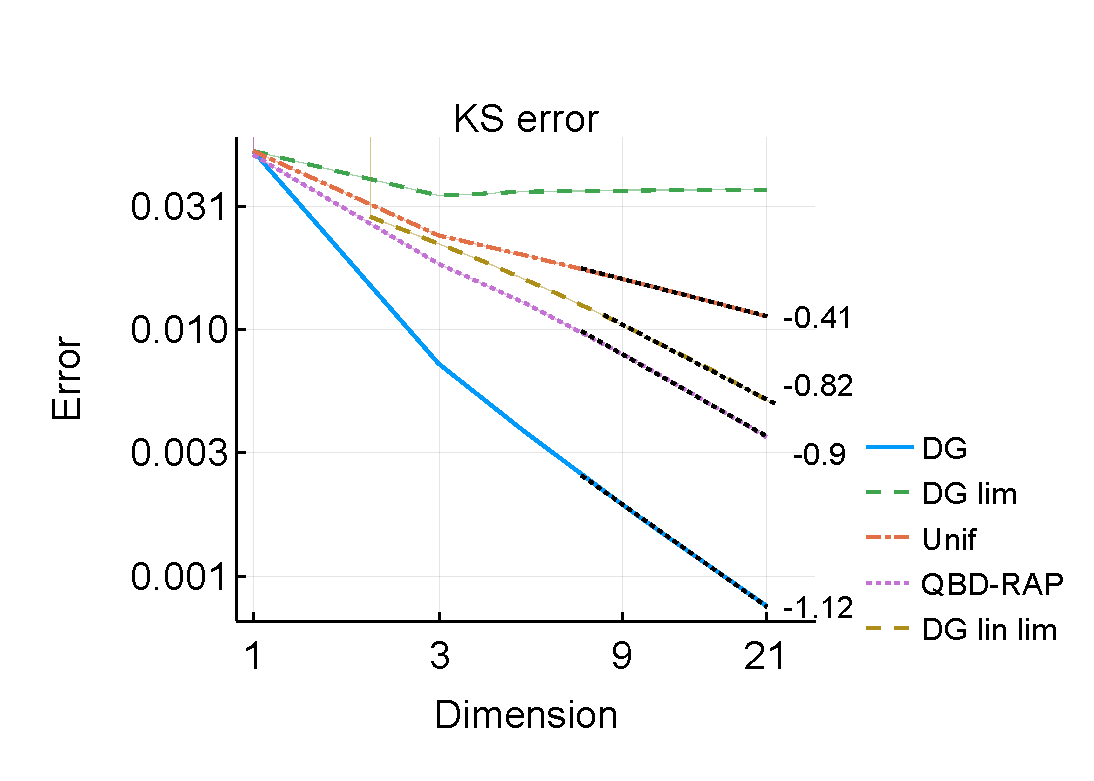
\includegraphics[width=0.5\textwidth,trim={0.75cm 0.8cm 0.25cm 1.25cm},clip]{chapter6/figs/hitting_times_model/hitting_times/exp/ks_error_formatted.pdf}%
	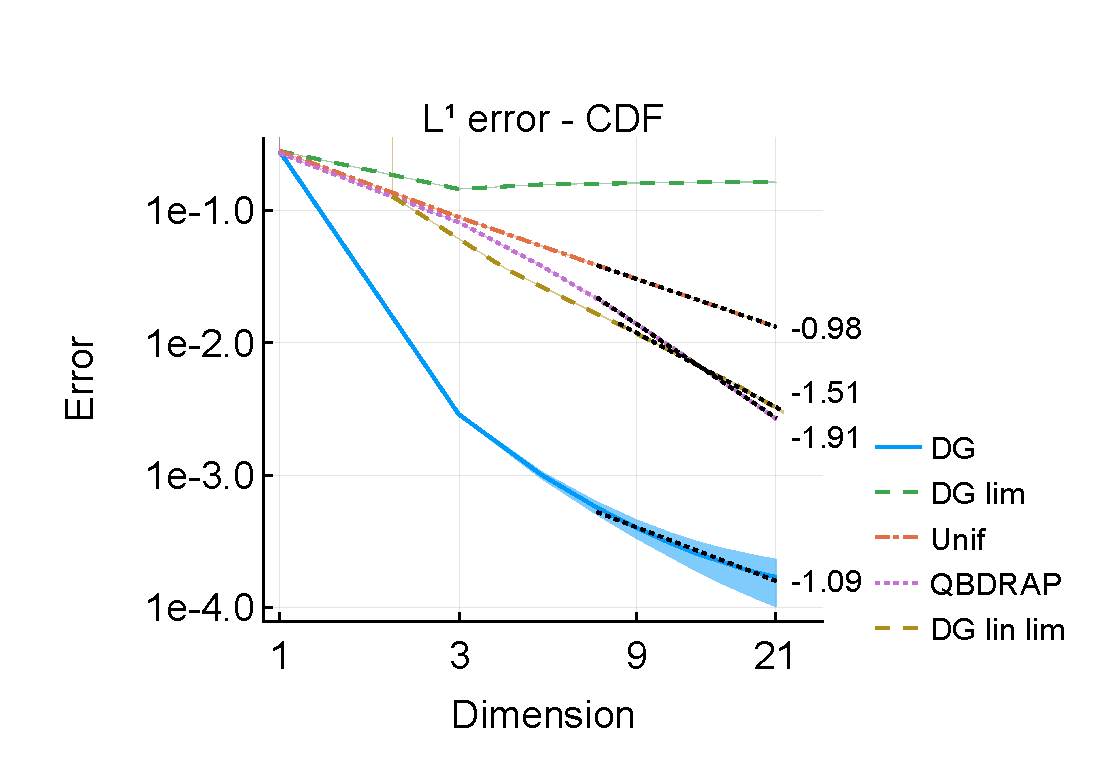
\includegraphics[width=0.5\textwidth,trim={0.75cm 0.8cm 0.25cm 1.25cm},clip]{chapter6/figs/hitting_times_model/hitting_times/exp/l1_cdf_error_formatted.pdf}
	\caption{KS (left) and \(L^1\) (right) errors between the simulated and approximated first hitting time CDFs in (\ref{eqn: hit cdf}) for Model~\ref{model: simple} with the exponential initial condition. The approximations were obtained via the DG method (blue solid line), DG method with Generalised MUSCL limiter (orange dashed line), uniformisation method (green dashed line) and QBD-RAP method (purple dotted line). Bootstrapped 90\% confidence intervals are shown by the lighter coloured bars surrounding the lines.}
	\label{fig: hitting time exp} 
\end{figure}
\begin{figure}[h]
	\centering 
	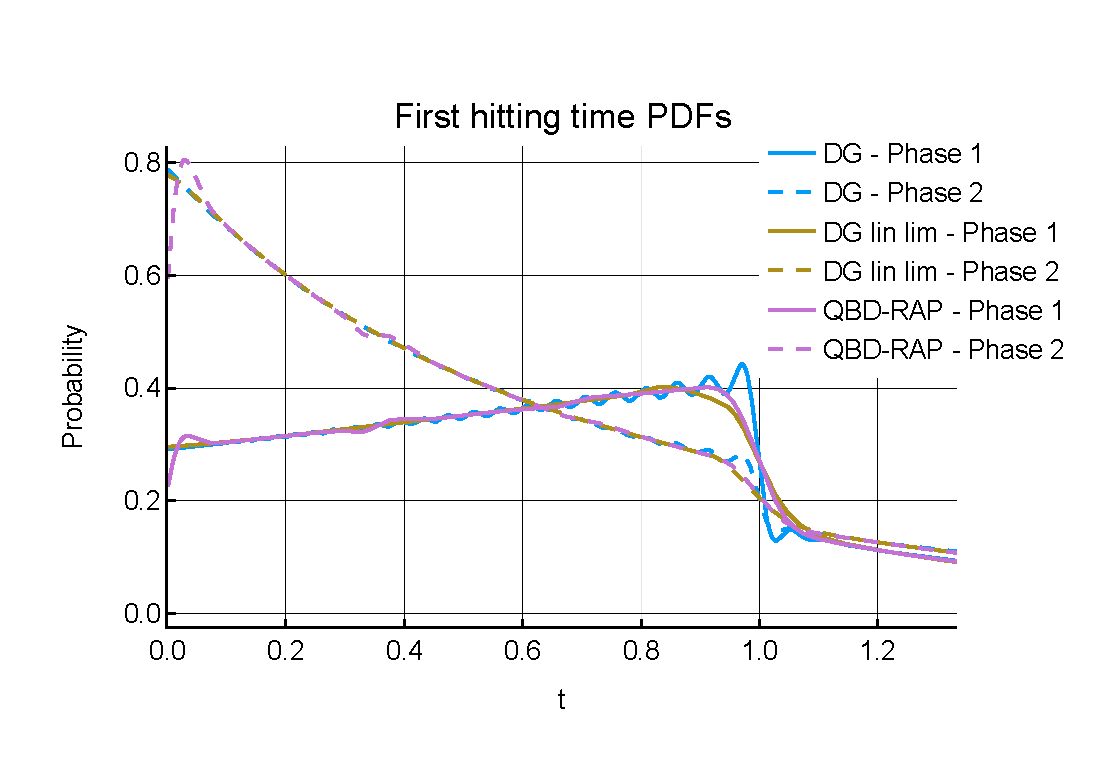
\includegraphics[width=0.8\textwidth,trim={0cm 1.25cm 0cm 1.25cm},clip]{chapter6/figs/hitting_times_model/hitting_times/exp/pdf_order21.pdf}%
	\caption{Approximations of the PDFs of the first hitting time for Model~\ref{model: simple} with the exponential initial condition. The blue line were obtained from the dimension-21 DG scheme and the purple lines were obtained from the dimension-21 QBD-RAP scheme. The DG scheme displays oscillations around the discontinuities at \(t=1\). } 
	\label{fig: hitting time oscillation exp} 
\end{figure}
\exampleFloatBarrier
\paragraph{Point mass initial condition}
Figure~\ref{fig: hitting time pm} shows the KS error (left) and \(L^1\) error for the CDF for the four different numerical approximation schemes applied to the hitting time problem with the point mass initial condition. The uniformisation and QBD-RAP method both appear to converge, with the QBD-RAP converging at a faster rate. The DG scheme with MUSCL limiter does not appear to converge, suggesting oscillations in the DG approximation. The DG scheme appears to converge fastest, however, oscillations are present in the DG approximation. In Figure~\ref{fig: hitting time oscillation} we plot the CDFs of the hitting time for Phase~1 obtained via the DG and QBD-RAP schemes, each using a dimension 21 basis. Observing Figure~\ref{fig: hitting time oscillation} the DG approximation clearly displays oscillations around and the discontinuity at \(t=1\). 
\begin{figure}[h]
	\centering
	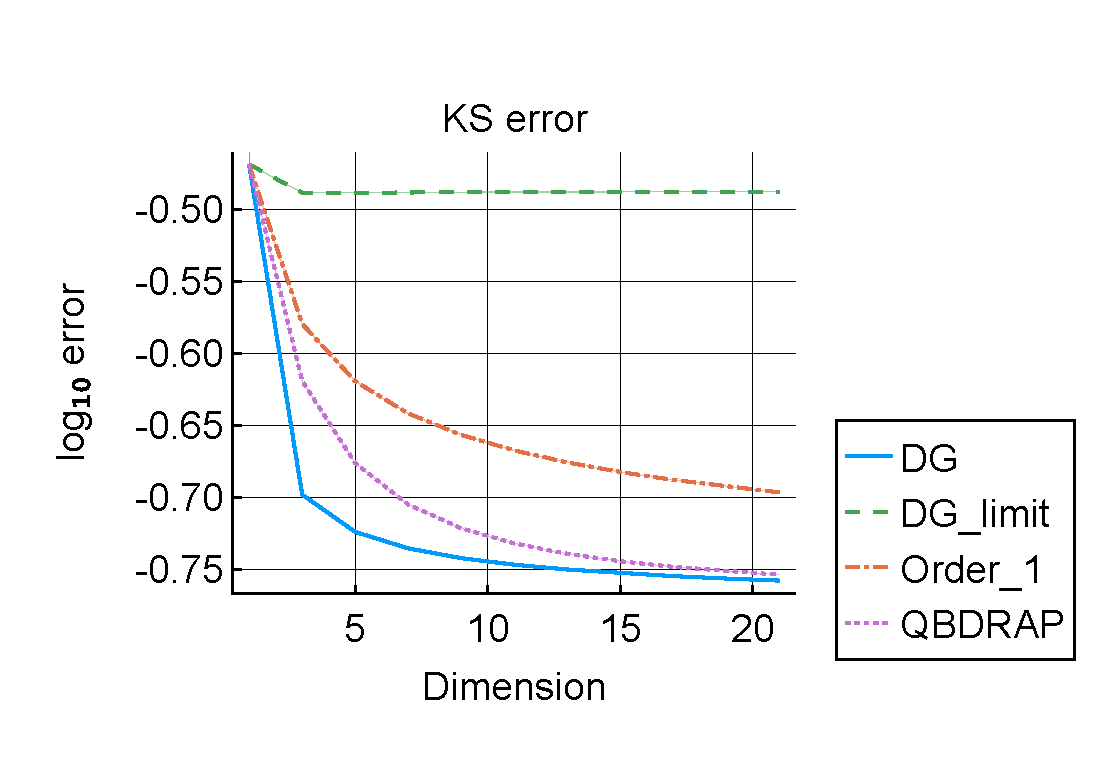
\includegraphics[width=0.5\textwidth,trim={0.75cm 0.8cm 0.25cm 1.25cm},clip]{chapter6/figs/hitting_times_model/hitting_times/point_mass/ks_error_formatted.pdf}%
	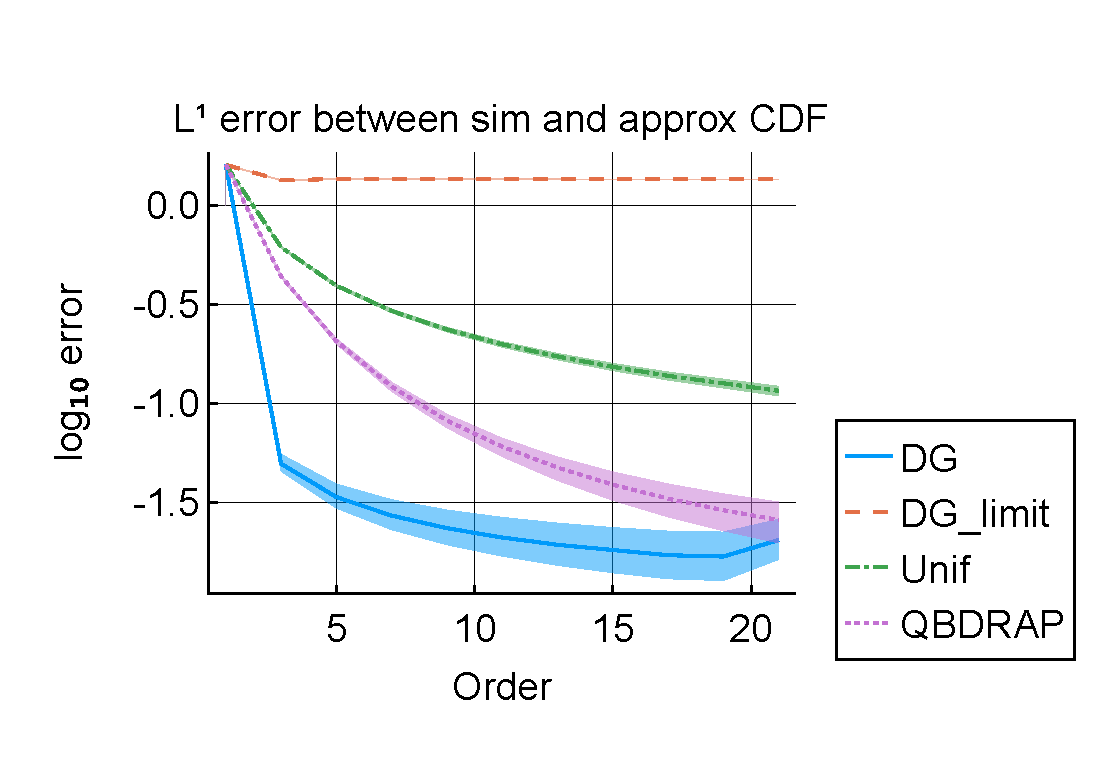
\includegraphics[width=0.5\textwidth,trim={0.75cm 0.8cm 0.25cm 1.25cm},clip]{chapter6/figs/hitting_times_model/hitting_times/point_mass/l1_cdf_error_formatted.pdf}
	\caption{KS (left) and \(L^1\) (right) errors between the simulated and approximated first hitting time CDFs in (\ref{eqn: hit cdf}) for Model~\ref{model: simple} with the point mass initial condition. The approximations were obtained via the DG method (blue solid line), DG method with Generalised MUSCL limiter (orange dashed line), uniformisation method (green dashed line) and QBD-RAP method (purple dotted line). Bootstrapped 90\% confidence intervals are shown by the lighter coloured bars surrounding the lines.} 
	\label{fig: hitting time pm} 
\end{figure}
\begin{figure}[h]
	\centering
	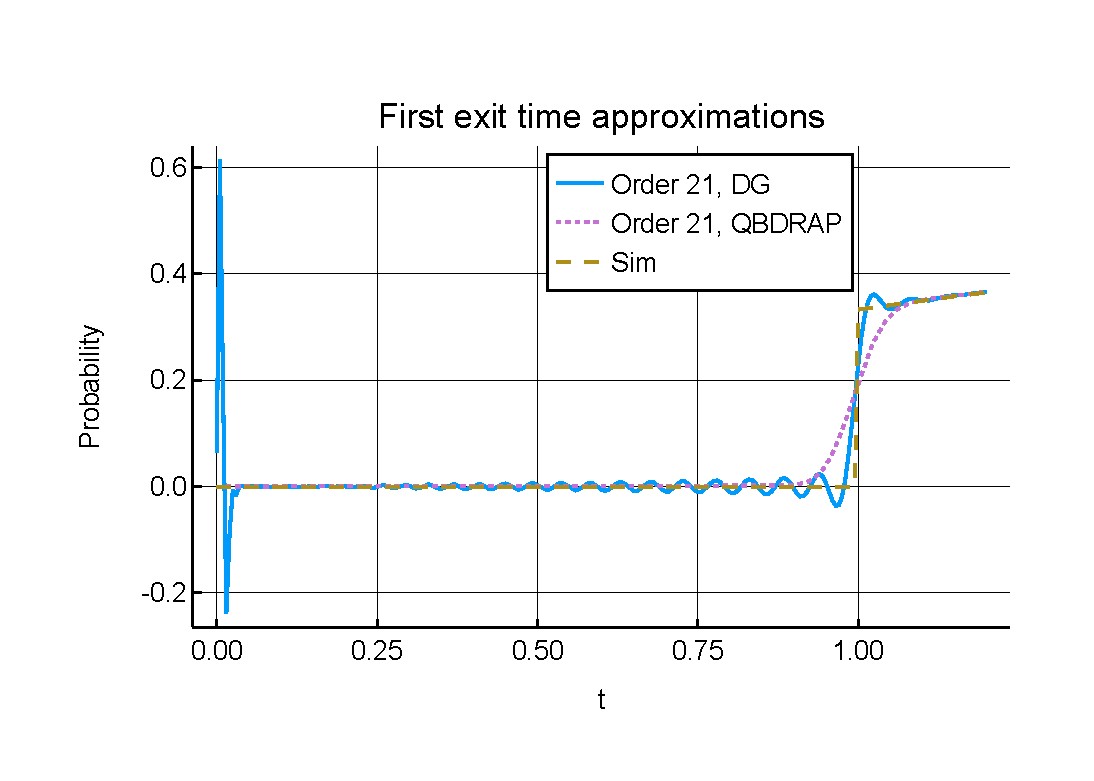
\includegraphics[width=0.8\textwidth,trim={0cm 1.25cm 0cm 1.25cm},clip]{chapter6/figs/hitting_times_model/hitting_times/point_mass/cdf_order21DG_and_sims.pdf}%
	\caption{Approximations of the CDF of the first hitting time in Phase~1 for Model~\ref{model: simple} with the point mass initial condition. The blue line was obtained from the dimension-21 DG scheme, the purple dotted line from the dimension-21 QBD-RAP scheme, and the gold dashed line is the empirical CDF obtained via simulation. The DG scheme displays oscillations. } 
	\label{fig: hitting time oscillation} 
\end{figure}

\FloatBarrier
\section{First-return distributions of fluid-fluid queues}\label{sec: ffq num}
Now consider the fluid-fluid queue model first analysed in \cite{blnos2022} which is a modified version of a model first presented in \cite{lnp13}. We refer the reader to \cite{blnos2022} for more on the DG method applied to this model. 
\begin{model}\label{model: ffq}
	Consider a stochastic fluid-fluid queue $\{(X(t),Y(t),\varphi(t))\}_{t\geq0},$ where $\{X(t)\}$ and $\{Y(t)\}$ represent the workloads in Buffers~1 and~2 at time $t \geq 0$, respectively, both driven by the phase $\{\varphi(t)\},$ which is a Markov chain on the state space $\mathcal{S} = \{11,10,01,00\}$. Both $\{X(t)\}$ and $\{Y(t)\}$ have a regulated boundary at 0. Here, the state $11$ indicates inputs to both buffers being \textnormal{\textsc{on}}, the state $00$ indicates both being \textnormal{\textsc{off}}, the state $10$ is when only the first input is \textnormal{\textsc{on}}, and the state $01$ is when only the second is \textnormal{\textsc{on}}. The input of Buffer~$k$ is switched from \textnormal{\textsc{on}} to \textnormal{\textsc{off}} with rate $\gamma_k$, and from \textnormal{\textsc{off}} to \textnormal{\textsc{on}} with rate $\beta_k$, for $k = 1, 2$. Thus, the infinitesimal generator $T$ for $\varphi(t)$ is given by 
	\begin{align*} 
		T = \left[ \begin{array}{cccc} -(\gamma_1 + \gamma_2) & \gamma_2 & \gamma_1 & 0 \\
							\beta_2 & -(\gamma_1 + \beta_2) & 0 & \gamma_1 \\
							\beta_1 & 0 & -(\gamma_2 + \beta_1) & \gamma_2 \\
							0 & \beta_1 &\beta_2 &-(\beta_1 + \beta_2)
	\end{array}\right].
	\end{align*} 

	The net rates of change for $X(t)$, denoted $c_i$, are given by 
	% 
	\begin{align*} 
	& (c_{11},c_{10},c_{01},c_{00})   =  \begin{array}{rrrr} 
	(\lambda_1-\theta_1,  & \lambda_1 -\theta_1, &  -\theta_1, & -\theta_1),
	\end{array}  
	\end{align*} 
	% 
	and the net rates of change for $Y(t)$, denoted $r_i$, are as follows  
	%  
	\begin{align*} 
	(r_{11},r_{10},r_{01},r_{00})  & = \left\{ \begin{array}{lrrrll}  
	% (\lambda_2 -\kappa, & \;\;\;\;0, & \lambda_2 - \kappa, &  \;\;\;\;0) & \text{if } X_t = 0,  Y_t = 0,\\
	%  \vspace*{-0.3cm} \\
												(\lambda_2 - \kappa, & \;\;\;-\kappa,  & \lambda_2 - \kappa, & -\kappa) &\text{if } X_t = 0, \\
												\vspace*{-0.3cm} \\
	%	(\lambda_2 -\theta_2,  &  0,  & \lambda_2 - \theta_2,  & \;\;\;\; 0) & \text{if } X_t \in (0,x^*), Y_t = 0,\\
	%											  \vspace*{-0.3cm} \\
		(\lambda_2 - \theta_2, & -\theta_2, & \lambda_2 - \theta_2, & -\theta_2) & \text{if } X_t \in (0,x^*),\\
												\vspace*{-0.3cm} \\
		(\;\;\;\;\;\;\; \lambda_2, & \;\;\;\;0, & \lambda_2, &  \;\;\;\;0) & \text{if } X_t \geq x^*. \end{array}
												\right.
	\end{align*} 

	For our numerical experiments, we use the parameter choices given in~\citep{lnp13}: 
	% 
		\begin{align} 
			\label{eqn:parameters}
		\gamma_1 & =11, \quad  \beta_1 = 1, \quad \lambda_1 = 12.48, \quad  \theta_1 = 1.6, \quad  \kappa = 2.6, \\
			\label{eqn:parameters-2}
		\gamma_2 & = 22, \quad \beta_2  = 1, \quad  \lambda_2 = 16.25, \quad \theta_2 = 1.0, \quad x^* = 1.6.
		\end{align} 
\end{model}
	
While the true problem has an unbounded domain $[0,\infty)$, the approximations require the domain of approximation to be a finite interval. Here we choose an upper bound of \(48\) and place a regulated boundary at the upper boundary. The effect of this truncation can be partly quantified by evaluating \(\lim\limits_{t\to\infty}\mathbb P\left(X(t) > 48\right)\approx 5.83 \times 10^{-9}\), \(i\in\calS\). 

We obtained approximations to the infinitesimal generator of the fluid queue \(\{(X(t),\varphi(t))\}_{t\geq 0}\) via the DG method, QBD-RAP method and uniformisation method, all of which used a cell width of \(\Delta=0.4\). The matrix resulting from the approximation is then used to approximate the first-return operator \(\mathbb\Psi(s)\) as discussed in Section~\ref{sec: intro Psi}. Due to the stochastic interpretation of the uniformisation and QBD-RAP schemes the approximations to \(\Psi(s)\) have a stochastic interpretation as the first-return probabilities of a fluid queue driven by a CTMC and QBD-RAP, respectively (see \cite[Chapter~7]{p2019} and \cite{bgnp2021} for details on the latter). For the DG method the approximation of \(\mathbb \Psi(s)\) is not as well-understood.\footnote{I believe that the resulting operator is a projection operator which, given an initial distribution, projects the distribution of \(X(\zeta_{Y}(\{0\}))\) on to a set of polynomial basis functions, much like the DG method itself.}

Ultimately, we approximate the first-return distribution 
\begin{align}\label{eqn: first return Y 1}
	\mathbb P(X(\zeta_{Y}(\{0\}))\leq x, \varphi(\zeta_{Y}(\{0\}))=i\mid \bs X(0)\sim \mu),
\end{align}
where we recall \(\zeta_{Y}(E) = \inf\{t>0\mid Y(t)\in E\}\) is the first hitting time of \(\{Y(t)\}\) on the set \(E\). For Model~\ref{model: ffq}, it is only possible for the process \(Y(t)\) to return to \(0\) at time \(t\) when \((X(t),\varphi(t))\in[0,1.6)\times \{10,00\}\), so we evaluate the approximations over this region only. We use a grid of 10,001 points on which we evaluate the approximations of the CDF in each phase. We consider first the initial distribution which is a point mass at \(Y(0)=0,\, X(0)=5,\, \varphi(0)=01\). 

For comparison, we simulated 5,000,000 realisations of the fluid-fluid queue and recorded the value of \(X\) and \(\varphi\) at the time of first return of the second fluid, \(Y\). The empirical approximation of (\ref{eqn: first return Y 1}) was then constructed, and error metrics for the difference between the empirical CDF and the approximations was computed. To account for Monte-Carlo errors we used a bootstrap with 1,000 bootstrap samples to construct 1,000 bootstrap samples of the error estimates and recorded the 5th and 95th percentiles of the error distribution. Each of the 1,000 bootstrap samples was constructed by resampling the original 5,000,000 realisations 5,000,000 times with replacement.

In Figure~\ref{fig: ffq return cts} we plot the error metrics for the approximations to the distribution (\ref{eqn: first return Y 1}). The DG method performs best converging rapidly until the error in the approximation scheme is swamped by other numerical errors. The QBD-RAP method is second best and the uniformisation scheme appears to be the slowest to converge. Here, the first return distribution appears to be smooth, hence we might expect the DG method to perform well. Note that there is a significant number other sources of error here; machine precision errors, errors in solving the matrix Ricatti equation to approximate \(\mathbb \Psi(s)\), errors from approximating error metrics (numerical integration/finding KS statistic), and truncation errors. Furthermore, for the QBD-RAP, since the parameters \(\bs \alpha,\,\bs S,\,\bs s\,\) and \(\bs D\) are found numerically, then there is another source of error from this. 
\begin{figure}[h]
	\centering
	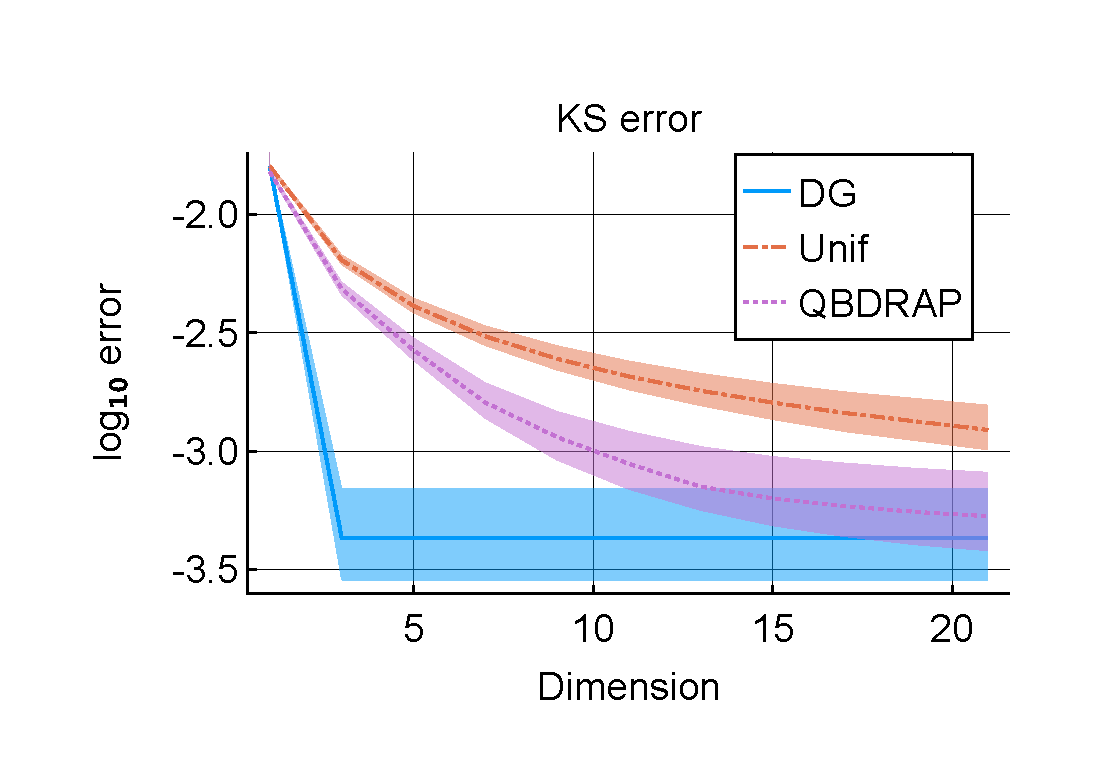
\includegraphics[width=0.5\textwidth,trim={0.75cm 0.8cm 0.25cm 1.25cm},clip]{chapter6/figs/ffq/cts/ks_error_formatted.pdf}%
	\includegraphics[width=0.5\textwidth,trim={0.75cm 0.8cm 0.25cm 1.25cm},clip]{chapter6/figs/ffq/cts/l1_cdf_error_formatted.pdf}
	\caption{KS (left) and \(L^1\) (right) errors between the simulated and approximated CDFs of \(X(\zeta_{Y}(\{0\}))\) in (\ref{eqn: first return Y 1}) for Model~\ref{model: ffq}. The approximations were obtained via the DG method (blue solid line), uniformisation method (green dashed line) and QBD-RAP method (purple dotted line). Bootstrapped 90\% confidence intervals are shown by the lighter coloured bars surrounding the lines.} 
	\label{fig: ffq return cts} 
\end{figure}
\begin{figure}[h]
	\centering
	\includegraphics[width=0.5\textwidth,trim={0.75cm 0.8cm 0.25cm 1.25cm},clip]{chapter6/figs/ffq/cts/l1_cell_probs_error_formatted.pdf}%
	\caption{Total error between the simulated and approximated probabilities of \(X(\zeta_{Y}(\{0\}))\) residing on each cell \(\mathcal D_k\) or at the boundary for Model~\ref{model: ffq}. The approximations were obtained via the DG method (blue solid line), uniformisation method (green dashed line) and QBD-RAP method (purple dotted line). Bootstrapped 90\% confidence intervals are shown by the lighter coloured bars surrounding the lines.} 
	\label{fig: ffq cell probs} 
\end{figure}
\exampleFloatBarrier
By modifying slightly Model~\ref{model: ffq}, we can construct a first return distribution which is discontinuous. 
\begin{model}\label{model: ffq2}
	Consider a fluid-fluid queue which is the same as Model~\ref{model: ffq} except 
	\begin{align}
		r_{00}(X(t)) = \begin{cases}
			-\kappa, & \mbox{ if }X(t)=0,\\
			-\theta_2, & \mbox{ if }X(t)=\in(0,x^*),\\
			\theta_2, & \mbox{ if }X(t)\geq x^*,
		\end{cases}
	\end{align}
	with an initial distribution which is a point-mass at \(Y(0)=0,\, X(0)=2, \varphi(0)=00\). 
\end{model}
As before, we use the DG, uniformisation and QBD-RAP methods to approximate the model, and compare to simulations. 

For Model~\ref{model: ffq2} there is a point mass at \(X(\zeta_{Y}(\{0\}))=1.2\) of magnitude \(e^{-(\beta_1+\beta_2)}\times 0.5\), which occurs when the phase remains in \(\varphi(t)=00\) for all \(t\in [0,\zeta_{Y}(\{0\})]\).

Figure~\ref{fig: ffq return discts} plots the error metrics for the first return distribution. Observing Figure~\ref{fig: ffq return discts} we see that the DG method performs well, followed by the QBD-RAP method, then the uniformisation method performs worst. However, the DG method results in an oscillatory solution with the CDF taking impossible values (decreasing at points) as shown in Figure~\ref{fig: ffq2 oscillation}
\begin{figure}[h]
	\centering
	\includegraphics[width=0.5\textwidth,trim={0.75cm 0.8cm 0.25cm 1.25cm},clip]{chapter6/figs/ffq/discts/ks_error_formatted.pdf}%
	\includegraphics[width=0.5\textwidth,trim={0.75cm 0.8cm 0.25cm 1.25cm},clip]{chapter6/figs/ffq/discts/l1_cdf_error_formatted.pdf}
	\caption{KS (left) and \(L^1\) (right) errors between the simulated and approximated CDFs of \(X(\zeta_{Y}(\{0\}))\) (Equation~\ref{eqn: first return Y 1}) for Model~\ref{model: ffq2}. The approximations were obtained via the DG method (blue solid line), uniformisation method (green dashed line) and QBD-RAP method (purple dotted line). Bootstrapped 90\% confidence intervals are shown by the lighter coloured bars surrounding the lines.} 
	\label{fig: ffq return discts} 
\end{figure} 
\begin{figure}[h]
	\centering
	\includegraphics[width=0.5\textwidth,trim={0.75cm 0.8cm 0.25cm 1.25cm},clip]{chapter6/figs/ffq/discts/l1_cell_probs_error_formatted.pdf}%
	\caption{Cell-wise error between the simulated and approximated probabilities of \(X(\zeta_{Y}(\{0\}))\) residing in each cell \(\mathcal D_k\) or at the boundary for Model~\ref{model: ffq2}. The approximations were obtained via the DG method (blue solid line), uniformisation method (green dashed line) and QBD-RAP method (purple dotted line). Bootstrapped 90\% confidence intervals are shown by the lighter coloured bars surrounding the lines.} 
	\label{fig: ffq2 cell probs} 
\end{figure}
\begin{figure}[h] 
	\centering
	\includegraphics[width=0.8\textwidth,trim={0cm 1.25cm 0cm 1.25cm},clip]{chapter6/figs/ffq/discts/phase_4_cdf.pdf}%
	\caption{Approximations of the CDF of the distribution of \(X\) at the time \(\zeta_Y(\{0\})\) in Phase~1 for Model~\ref{model: ffq2}. The blue line was obtained from the dimension-21 DG scheme, the purple dotted line from the dimension-21 QBD-RAP scheme, and the gold dashed line is the empirical CDF obtained via simulation. The DG scheme displays oscillations around the discontinuity. } 
	\label{fig: ffq2 oscillation} 
\end{figure}
\FloatBarrier


\section{Discussion}

The structure of this chapter is as follows. In Section~\ref{sec: recon num} we compute approximations to various initial conditions for the different methods and observe their performance at approximating the initial condition, which allows us to instrument the performance of the reconstruction methods without considering a specific model or any dynamics of the problem. In Section~\ref{sec: wave num} we investigate a simple travelling wave problem with various initial conditions. For this problem the dynamics are deterministic, which allows us to instrument the ability of the schemes to approximate the flow of probability across cells without any stochastic dynamics. Next, we investigate a simple fluid queue with two phases. Section~\ref{sec:stat} investigates the ability of the methods to approximate the stationary distribution of the model, Section~\ref{sec: transient approx} investigates the ability of the schemes to approximate the transient distribution of the fluid queue for two initial conditions, and Section~\ref{sec: return approx} investigates the ability of the methods to approximate the first hitting time of the fluid level on the boundary of the interval \([0,1]\). Section~\ref{sec: ffq num} approximates the distribution of \(\{(X(t),\varphi(t))\}\) at the time at which \(\{Y(t)\}\) first returns to \(0\) for two simple fluid-fluid queue models.  

In this chapter we have numerically investigated some properties of the QBD-RAP approximation scheme and compared it to existing methods; the uniformisation scheme of \cite{bo2013} and the discontinuous Galerkin scheme. In general, the numerical experiments show that, for problems with discontinuities, the DG approximation can exhibit oscillations, while the QBD-RAP and uniformisation approximations avoid this and, of the latter two, the QBD-RAP scheme often converges faster. To avoid the problems of oscillations we can sometimes employ a \emph{slope limiter} with the DG scheme, which effectively reduces the scheme to linear in the regions where oscillations are detected. The numerical experiments demonstrate a loss of accuracy in the DG approximation when a slope limiter is used for a purely discontinuous problem. Moreover, for the application of the methods to fluid-fluid queues, there is no obvious way to apply the concept of a slope limiter. %When the slope limiter detects oscillations in the approximate solution, it reduces the DG scheme to linear in the region surrounding the oscillations, otherwise, the slope limiter leaves the solution unchanged. Thus, the slope limiter permits high-order approximations away from oscillations, while also removing oscillations. 
In general, we observe that the smoother the problem is the better the performance of the DG method, and it emphatically outperforms the other two methods. 

As a first step in the numerical experiments, in Section~\ref{sec: recon num}, we examined the ability of each method to approximate different initial conditions. For the DG method, this is equivalent to a projection of the initial condition on to a set of basis polynomials. For the uniformisation method this is equivalent to projecting the initial condition on to a basis of constant functions. For the QBD-RAP method the approximation of the initial condition is as described in Sections~\ref{sec: initial conditions} and \ref{sec: closing}. Section~\ref{sec: comp} demonstrates that the DG scheme (projection) can result in oscillations and negative regions in the approximation when the initial condition is discontinuous. The uniformisation and QBD-RAP methods avoid this problem, but appear to have higher errors and the QBD-RAP method appears to have the largest errors. For discontinuous initial conditions the rates of convergence are comparable for all three methods. However, when the initial condition to be approximated is sufficiently smooth, then the DG approximation is superior. 

Next, in Section~\ref{sec: wave num}, we instrumented the performance of approximations for a simple travelling wave problem with various initial conditions. For this problem the solution is given in terms of the initial condition by \(f(x,t) = f(x-t,0)\). This model is useful as it allows us to instrument the ability of the methods to capture the flow of probability without stochastic dynamics. Once again, for discontinuous problems, the DG method can display oscillations, while the other methods (DG with slope limiter, uniformisation and QBD-RAP methods) avoid oscillations. Further, for discontinuous problems the rates of convergence of the QBD-RAP and DG methods can be similar. For smooth problems the DG method is superior. Interestingly, even though the QBD-RAP method performed worst for approximating initial conditions in the previous section, it outperformed the uniformisation method for this model, demonstrating that the QBD-RAP method can capture the dynamics of the flow of probability better than the uniformisation method.

We then instrumented the performance of the approximations on a simple fluid queue with two phases. First, in Section~\ref{sec:stat}, we looked at the stationary distribution, which is known to be smooth. Since the problem is smooth, then the DG method was superior as expected. Of the uniformisation and QBD-RAP methods, the QBD-RAP method gives more accurate solutions. In Section~\ref{sec: transient approx} we turned our attention to approximating transient distributions for the same models and consider two different initial conditions, a point-mass and an exponential initial condition. The discontinuous initial condition results in a discontinuous transient distribution. As for the exponential initial condition, this example demonstrates that, even if the initial condition appears `nice', it can still result in discontinuous, or non-differetiable solutions. The numerical evidence suggests that the DG method can display oscillations, while the other methods do not. The DG method with slope limiter detects the oscillations and reduces the method to linear. Of the uniformisation and QBD-RAP methods, the latter performs better. 

Next, Section~\ref{sec: return approx} looked at hitting times for the same fluid queue with two initial conditions, an exponential initial condition and a point-mass. We looked at the hitting time of the fluid level on the points \(\{0\}\) and \(\{1\}\). For this problem there is never any in-flow of mass at the boundaries of the interval and so, for a solution to be continuous, the initial condition needs to be chosen carefully, otherwise discontinuities in the transient distribution may result, as is the case for both initial conditions here. The numerical results suggest that, due to the discontinuities in the problems, the DG method may display oscillations. Since the uniformisation and QBD-RAP methods can handle discontinuities, they perform as expected, with the QBD-RAP method performing better than the uniformisation. 

Lastly, we applied the DG, uniformisation and QBD-RAP methods to two simple fluid-fluid queues in Section~\ref{sec: ffq num}. In the first fluid-fluid queue, which appears to have a smooth solution, the DG method performs very well. Of the two positivity preserving schemes the QBD-RAP scheme performs better than the uniformisation scheme. In the second example, which has a discontinuity, the DG method produces the lowest errors, but exhibits oscillations in the solution. The QBD-RAP and uniformisation schemes do not produce oscillations and, of the two, the QBD-RAP method performs best. 

In conclusion, when the problem is known to be smooth, the DG method is very likely to produce excellent results. However, for discontinuous problems, the method can show oscillations and infeasible or negative regions of the solution. The slope limiter overcomes this, but reduces the accuracy of the DG method to linear near discontinuities, sometimes severely affecting the quality of the approximation. The uniformisation and QBD-RAP methods are alternative approximation schemes which exhibit larger errors, but avoid oscillatory solutions and guarantee a non-decreasing approximation of the CDF. Of the uniformisation and QBD-RAP methods, the latter often to produced lower errors. 
